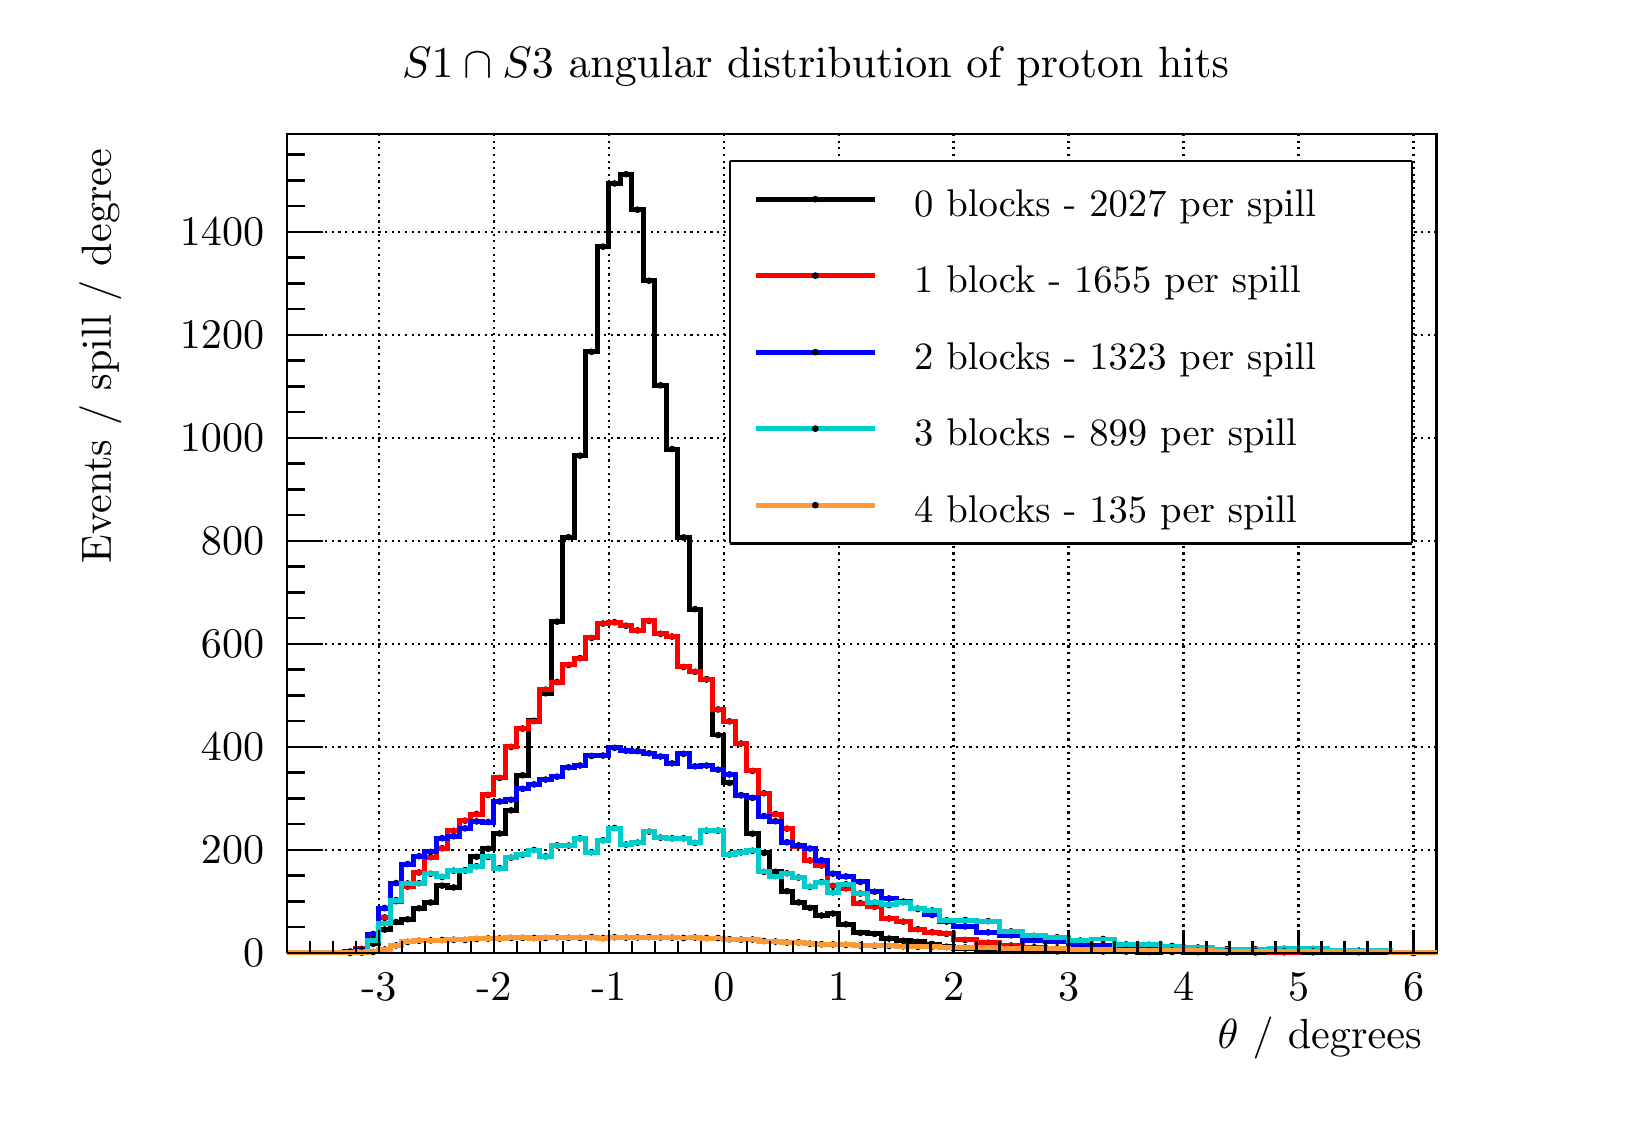
\begin{tikzpicture}
\pgfdeclareplotmark{cross} {
\pgfpathmoveto{\pgfpoint{-0.3\pgfplotmarksize}{\pgfplotmarksize}}
\pgfpathlineto{\pgfpoint{+0.3\pgfplotmarksize}{\pgfplotmarksize}}
\pgfpathlineto{\pgfpoint{+0.3\pgfplotmarksize}{0.3\pgfplotmarksize}}
\pgfpathlineto{\pgfpoint{+1\pgfplotmarksize}{0.3\pgfplotmarksize}}
\pgfpathlineto{\pgfpoint{+1\pgfplotmarksize}{-0.3\pgfplotmarksize}}
\pgfpathlineto{\pgfpoint{+0.3\pgfplotmarksize}{-0.3\pgfplotmarksize}}
\pgfpathlineto{\pgfpoint{+0.3\pgfplotmarksize}{-1.\pgfplotmarksize}}
\pgfpathlineto{\pgfpoint{-0.3\pgfplotmarksize}{-1.\pgfplotmarksize}}
\pgfpathlineto{\pgfpoint{-0.3\pgfplotmarksize}{-0.3\pgfplotmarksize}}
\pgfpathlineto{\pgfpoint{-1.\pgfplotmarksize}{-0.3\pgfplotmarksize}}
\pgfpathlineto{\pgfpoint{-1.\pgfplotmarksize}{0.3\pgfplotmarksize}}
\pgfpathlineto{\pgfpoint{-0.3\pgfplotmarksize}{0.3\pgfplotmarksize}}
\pgfpathclose
\pgfusepathqstroke
}
\pgfdeclareplotmark{cross*} {
\pgfpathmoveto{\pgfpoint{-0.3\pgfplotmarksize}{\pgfplotmarksize}}
\pgfpathlineto{\pgfpoint{+0.3\pgfplotmarksize}{\pgfplotmarksize}}
\pgfpathlineto{\pgfpoint{+0.3\pgfplotmarksize}{0.3\pgfplotmarksize}}
\pgfpathlineto{\pgfpoint{+1\pgfplotmarksize}{0.3\pgfplotmarksize}}
\pgfpathlineto{\pgfpoint{+1\pgfplotmarksize}{-0.3\pgfplotmarksize}}
\pgfpathlineto{\pgfpoint{+0.3\pgfplotmarksize}{-0.3\pgfplotmarksize}}
\pgfpathlineto{\pgfpoint{+0.3\pgfplotmarksize}{-1.\pgfplotmarksize}}
\pgfpathlineto{\pgfpoint{-0.3\pgfplotmarksize}{-1.\pgfplotmarksize}}
\pgfpathlineto{\pgfpoint{-0.3\pgfplotmarksize}{-0.3\pgfplotmarksize}}
\pgfpathlineto{\pgfpoint{-1.\pgfplotmarksize}{-0.3\pgfplotmarksize}}
\pgfpathlineto{\pgfpoint{-1.\pgfplotmarksize}{0.3\pgfplotmarksize}}
\pgfpathlineto{\pgfpoint{-0.3\pgfplotmarksize}{0.3\pgfplotmarksize}}
\pgfpathclose
\pgfusepathqfillstroke
}
\pgfdeclareplotmark{newstar} {
\pgfpathmoveto{\pgfqpoint{0pt}{\pgfplotmarksize}}
\pgfpathlineto{\pgfqpointpolar{44}{0.5\pgfplotmarksize}}
\pgfpathlineto{\pgfqpointpolar{18}{\pgfplotmarksize}}
\pgfpathlineto{\pgfqpointpolar{-20}{0.5\pgfplotmarksize}}
\pgfpathlineto{\pgfqpointpolar{-54}{\pgfplotmarksize}}
\pgfpathlineto{\pgfqpointpolar{-90}{0.5\pgfplotmarksize}}
\pgfpathlineto{\pgfqpointpolar{234}{\pgfplotmarksize}}
\pgfpathlineto{\pgfqpointpolar{198}{0.5\pgfplotmarksize}}
\pgfpathlineto{\pgfqpointpolar{162}{\pgfplotmarksize}}
\pgfpathlineto{\pgfqpointpolar{134}{0.5\pgfplotmarksize}}
\pgfpathclose
\pgfusepathqstroke
}
\pgfdeclareplotmark{newstar*} {
\pgfpathmoveto{\pgfqpoint{0pt}{\pgfplotmarksize}}
\pgfpathlineto{\pgfqpointpolar{44}{0.5\pgfplotmarksize}}
\pgfpathlineto{\pgfqpointpolar{18}{\pgfplotmarksize}}
\pgfpathlineto{\pgfqpointpolar{-20}{0.5\pgfplotmarksize}}
\pgfpathlineto{\pgfqpointpolar{-54}{\pgfplotmarksize}}
\pgfpathlineto{\pgfqpointpolar{-90}{0.5\pgfplotmarksize}}
\pgfpathlineto{\pgfqpointpolar{234}{\pgfplotmarksize}}
\pgfpathlineto{\pgfqpointpolar{198}{0.5\pgfplotmarksize}}
\pgfpathlineto{\pgfqpointpolar{162}{\pgfplotmarksize}}
\pgfpathlineto{\pgfqpointpolar{134}{0.5\pgfplotmarksize}}
\pgfpathclose
\pgfusepathqfillstroke
}
\definecolor{c}{rgb}{1,1,1};
\draw [color=c, fill=c] (0,0) rectangle (20,13.5143);
\draw [color=c, fill=c] (3.28571,1.77143) rectangle (17.8857,12.1714);
\definecolor{c}{rgb}{0,0,0};
\draw [c,line width=0.9] (3.28571,1.77143) -- (3.28571,12.1714) -- (17.8857,12.1714) -- (17.8857,1.77143) -- (3.28571,1.77143);
\definecolor{c}{rgb}{1,1,1};
\draw [color=c, fill=c] (3.28571,1.77143) rectangle (17.8857,12.1714);
\definecolor{c}{rgb}{0,0,0};
\draw [c,line width=0.9] (3.28571,1.77143) -- (3.28571,12.1714) -- (17.8857,12.1714) -- (17.8857,1.77143) -- (3.28571,1.77143);
\draw [c,line width=0.9] (3.28571,1.77143) -- (17.8857,1.77143);
\draw [c,dash pattern=on 0.80pt off 1.60pt ,line width=0.9] (4.45371,12.1714) -- (4.45371,1.77143);
\draw [c,dash pattern=on 0.80pt off 1.60pt ,line width=0.9] (5.91371,12.1714) -- (5.91371,1.77143);
\draw [c,dash pattern=on 0.80pt off 1.60pt ,line width=0.9] (7.37371,12.1714) -- (7.37371,1.77143);
\draw [c,dash pattern=on 0.80pt off 1.60pt ,line width=0.9] (8.83371,12.1714) -- (8.83371,1.77143);
\draw [c,dash pattern=on 0.80pt off 1.60pt ,line width=0.9] (10.2937,12.1714) -- (10.2937,1.77143);
\draw [c,dash pattern=on 0.80pt off 1.60pt ,line width=0.9] (11.7537,12.1714) -- (11.7537,1.77143);
\draw [c,dash pattern=on 0.80pt off 1.60pt ,line width=0.9] (13.2137,12.1714) -- (13.2137,1.77143);
\draw [c,dash pattern=on 0.80pt off 1.60pt ,line width=0.9] (14.6737,12.1714) -- (14.6737,1.77143);
\draw [c,dash pattern=on 0.80pt off 1.60pt ,line width=0.9] (16.1337,12.1714) -- (16.1337,1.77143);
\draw [c,dash pattern=on 0.80pt off 1.60pt ,line width=0.9] (17.5937,12.1714) -- (17.5937,1.77143);
\draw [c,dash pattern=on 0.80pt off 1.60pt ,line width=0.9] (4.45371,12.1714) -- (4.45371,1.77143);
\draw [c,dash pattern=on 0.80pt off 1.60pt ,line width=0.9] (17.5937,12.1714) -- (17.5937,1.77143);
\draw [c,line width=0.9] (3.28571,1.77143) -- (3.28571,12.1714);
\draw [c,dash pattern=on 0.80pt off 1.60pt ,line width=0.9] (17.8857,1.77143) -- (3.28571,1.77143);
\draw [c,dash pattern=on 0.80pt off 1.60pt ,line width=0.9] (17.8857,3.07955) -- (3.28571,3.07955);
\draw [c,dash pattern=on 0.80pt off 1.60pt ,line width=0.9] (17.8857,4.38766) -- (3.28571,4.38766);
\draw [c,dash pattern=on 0.80pt off 1.60pt ,line width=0.9] (17.8857,5.69578) -- (3.28571,5.69578);
\draw [c,dash pattern=on 0.80pt off 1.60pt ,line width=0.9] (17.8857,7.0039) -- (3.28571,7.0039);
\draw [c,dash pattern=on 0.80pt off 1.60pt ,line width=0.9] (17.8857,8.31201) -- (3.28571,8.31201);
\draw [c,dash pattern=on 0.80pt off 1.60pt ,line width=0.9] (17.8857,9.62013) -- (3.28571,9.62013);
\draw [c,dash pattern=on 0.80pt off 1.60pt ,line width=0.9] (17.8857,10.9282) -- (3.28571,10.9282);
\draw [c,dash pattern=on 0.80pt off 1.60pt ,line width=0.9] (17.8857,10.9282) -- (3.28571,10.9282);
\definecolor{c}{rgb}{0,0,0.6};
\draw [c,line width=0.9] (3.28571,1.77143) -- (3.43171,1.77143) -- (3.43171,1.77143) -- (3.57771,1.77143) -- (3.57771,1.77143) -- (3.72371,1.77143) -- (3.72371,1.77143) -- (3.86971,1.77143) -- (3.86971,1.77143) -- (4.01571,1.77143) --
 (4.01571,1.77143) -- (4.16171,1.77143) -- (4.16171,1.77143) -- (4.30771,1.77143) -- (4.30771,1.77143) -- (4.45371,1.77143) -- (4.45371,1.77143) -- (4.59971,1.77143) -- (4.59971,1.77143) -- (4.74571,1.77143) -- (4.74571,1.77143) -- (4.89171,1.77143)
 -- (4.89171,1.77143) -- (5.03771,1.77143) -- (5.03771,1.77143) -- (5.18371,1.77143) -- (5.18371,1.77143) -- (5.32971,1.77143) -- (5.32971,1.77143) -- (5.47571,1.77143) -- (5.47571,1.77143) -- (5.62171,1.77143) -- (5.62171,1.77143) --
 (5.76771,1.77143) -- (5.76771,1.77143) -- (5.91371,1.77143) -- (5.91371,1.77143) -- (6.05971,1.77143) -- (6.05971,1.77143) -- (6.20571,1.77143) -- (6.20571,1.77143) -- (6.35171,1.77143) -- (6.35171,1.77143) -- (6.49771,1.77143) -- (6.49771,1.77143)
 -- (6.64371,1.77143) -- (6.64371,1.77143) -- (6.78971,1.77143) -- (6.78971,1.77143) -- (6.93571,1.77143) -- (6.93571,1.77143) -- (7.08171,1.77143) -- (7.08171,1.77143) -- (7.22771,1.77143) -- (7.22771,1.77143) -- (7.37371,1.77143) --
 (7.37371,1.77143) -- (7.51971,1.77143) -- (7.51971,1.77143) -- (7.66571,1.77143) -- (7.66571,1.77143) -- (7.81171,1.77143) -- (7.81171,1.77143) -- (7.95771,1.77143) -- (7.95771,1.77143) -- (8.10371,1.77143) -- (8.10371,1.77143) -- (8.24971,1.77143)
 -- (8.24971,1.77143) -- (8.39571,1.77143) -- (8.39571,1.77143) -- (8.54171,1.77143) -- (8.54171,1.77143) -- (8.68771,1.77143) -- (8.68771,1.77143) -- (8.83371,1.77143) -- (8.83371,1.77143) -- (8.97971,1.77143) -- (8.97971,1.77143) --
 (9.12571,1.77143) -- (9.12571,1.77143) -- (9.27171,1.77143) -- (9.27171,1.77143) -- (9.41771,1.77143) -- (9.41771,1.77143) -- (9.56371,1.77143) -- (9.56371,1.77143) -- (9.70971,1.77143) -- (9.70971,1.77143) -- (9.85571,1.77143) -- (9.85571,1.77143)
 -- (10.0017,1.77143) -- (10.0017,1.77143) -- (10.1477,1.77143) -- (10.1477,1.77143) -- (10.2937,1.77143) -- (10.2937,1.77143) -- (10.4762,1.77143) -- (10.4762,1.77143) -- (10.6587,1.77143) -- (10.6587,1.77143) -- (10.8412,1.77143) --
 (10.8412,1.77143) -- (11.0237,1.77143) -- (11.0237,1.77143) -- (11.2062,1.77143) -- (11.2062,1.77143) -- (11.3887,1.77143) -- (11.3887,1.77143) -- (11.5712,1.77143) -- (11.5712,1.77143) -- (11.7537,1.77143) -- (11.7537,1.77143) -- (12.0457,1.77143)
 -- (12.0457,1.77143) -- (12.3377,1.77143) -- (12.3377,1.77143) -- (12.6297,1.77143) -- (12.6297,1.77143) -- (12.9217,1.77143) -- (12.9217,1.77143) -- (13.2137,1.77143) -- (13.2137,1.77143) -- (13.5057,1.77143) -- (13.5057,1.77143) --
 (13.7977,1.77143) -- (13.7977,1.77143) -- (14.0897,1.77143) -- (14.0897,1.77143) -- (14.3817,1.77143) -- (14.3817,1.77143) -- (14.6737,1.77143) -- (14.6737,1.77143) -- (15.0387,1.77143) -- (15.0387,1.77143) -- (15.4037,1.77143) -- (15.4037,1.77143)
 -- (15.7687,1.77143) -- (15.7687,1.77143) -- (16.1337,1.77143) -- (16.1337,1.77143) -- (16.4987,1.77143) -- (16.4987,1.77143) -- (17.3017,1.77143) -- (17.3017,1.77143) -- (17.8857,1.77143);
\definecolor{c}{rgb}{0,0,0};
\draw [c,line width=0.9] (3.28571,1.77143) -- (17.8857,1.77143);
\draw [c,line width=0.9] (4.45371,2.06739) -- (4.45371,1.77143);
\draw [c,line width=0.9] (4.74571,1.91941) -- (4.74571,1.77143);
\draw [c,line width=0.9] (5.03771,1.91941) -- (5.03771,1.77143);
\draw [c,line width=0.9] (5.32971,1.91941) -- (5.32971,1.77143);
\draw [c,line width=0.9] (5.62171,1.91941) -- (5.62171,1.77143);
\draw [c,line width=0.9] (5.91371,2.06739) -- (5.91371,1.77143);
\draw [c,line width=0.9] (6.20571,1.91941) -- (6.20571,1.77143);
\draw [c,line width=0.9] (6.49771,1.91941) -- (6.49771,1.77143);
\draw [c,line width=0.9] (6.78971,1.91941) -- (6.78971,1.77143);
\draw [c,line width=0.9] (7.08171,1.91941) -- (7.08171,1.77143);
\draw [c,line width=0.9] (7.37371,2.06739) -- (7.37371,1.77143);
\draw [c,line width=0.9] (7.66571,1.91941) -- (7.66571,1.77143);
\draw [c,line width=0.9] (7.95771,1.91941) -- (7.95771,1.77143);
\draw [c,line width=0.9] (8.24971,1.91941) -- (8.24971,1.77143);
\draw [c,line width=0.9] (8.54171,1.91941) -- (8.54171,1.77143);
\draw [c,line width=0.9] (8.83371,2.06739) -- (8.83371,1.77143);
\draw [c,line width=0.9] (9.12571,1.91941) -- (9.12571,1.77143);
\draw [c,line width=0.9] (9.41771,1.91941) -- (9.41771,1.77143);
\draw [c,line width=0.9] (9.70971,1.91941) -- (9.70971,1.77143);
\draw [c,line width=0.9] (10.0017,1.91941) -- (10.0017,1.77143);
\draw [c,line width=0.9] (10.2937,2.06739) -- (10.2937,1.77143);
\draw [c,line width=0.9] (10.5857,1.91941) -- (10.5857,1.77143);
\draw [c,line width=0.9] (10.8777,1.91941) -- (10.8777,1.77143);
\draw [c,line width=0.9] (11.1697,1.91941) -- (11.1697,1.77143);
\draw [c,line width=0.9] (11.4617,1.91941) -- (11.4617,1.77143);
\draw [c,line width=0.9] (11.7537,2.06739) -- (11.7537,1.77143);
\draw [c,line width=0.9] (12.0457,1.91941) -- (12.0457,1.77143);
\draw [c,line width=0.9] (12.3377,1.91941) -- (12.3377,1.77143);
\draw [c,line width=0.9] (12.6297,1.91941) -- (12.6297,1.77143);
\draw [c,line width=0.9] (12.9217,1.91941) -- (12.9217,1.77143);
\draw [c,line width=0.9] (13.2137,2.06739) -- (13.2137,1.77143);
\draw [c,line width=0.9] (13.5057,1.91941) -- (13.5057,1.77143);
\draw [c,line width=0.9] (13.7977,1.91941) -- (13.7977,1.77143);
\draw [c,line width=0.9] (14.0897,1.91941) -- (14.0897,1.77143);
\draw [c,line width=0.9] (14.3817,1.91941) -- (14.3817,1.77143);
\draw [c,line width=0.9] (14.6737,2.06739) -- (14.6737,1.77143);
\draw [c,line width=0.9] (14.9657,1.91941) -- (14.9657,1.77143);
\draw [c,line width=0.9] (15.2577,1.91941) -- (15.2577,1.77143);
\draw [c,line width=0.9] (15.5497,1.91941) -- (15.5497,1.77143);
\draw [c,line width=0.9] (15.8417,1.91941) -- (15.8417,1.77143);
\draw [c,line width=0.9] (16.1337,2.06739) -- (16.1337,1.77143);
\draw [c,line width=0.9] (16.4257,1.91941) -- (16.4257,1.77143);
\draw [c,line width=0.9] (16.7177,1.91941) -- (16.7177,1.77143);
\draw [c,line width=0.9] (17.0097,1.91941) -- (17.0097,1.77143);
\draw [c,line width=0.9] (17.3017,1.91941) -- (17.3017,1.77143);
\draw [c,line width=0.9] (17.5937,2.06739) -- (17.5937,1.77143);
\draw [c,line width=0.9] (4.45371,2.06739) -- (4.45371,1.77143);
\draw [c,line width=0.9] (4.16171,1.91941) -- (4.16171,1.77143);
\draw [c,line width=0.9] (3.86971,1.91941) -- (3.86971,1.77143);
\draw [c,line width=0.9] (3.57771,1.91941) -- (3.57771,1.77143);
\draw [c,line width=0.9] (17.5937,2.06739) -- (17.5937,1.77143);
\draw [anchor=base] (4.45371,1.16329) node[scale=1.52295, color=c, rotate=0]{-3};
\draw [anchor=base] (5.91371,1.16329) node[scale=1.52295, color=c, rotate=0]{-2};
\draw [anchor=base] (7.37371,1.16329) node[scale=1.52295, color=c, rotate=0]{-1};
\draw [anchor=base] (8.83371,1.16329) node[scale=1.52295, color=c, rotate=0]{0};
\draw [anchor=base] (10.2937,1.16329) node[scale=1.52295, color=c, rotate=0]{1};
\draw [anchor=base] (11.7537,1.16329) node[scale=1.52295, color=c, rotate=0]{2};
\draw [anchor=base] (13.2137,1.16329) node[scale=1.52295, color=c, rotate=0]{3};
\draw [anchor=base] (14.6737,1.16329) node[scale=1.52295, color=c, rotate=0]{4};
\draw [anchor=base] (16.1337,1.16329) node[scale=1.52295, color=c, rotate=0]{5};
\draw [anchor=base] (17.5937,1.16329) node[scale=1.52295, color=c, rotate=0]{6};
\draw [anchor= east] (17.8857,0.690286) node[scale=1.52295, color=c, rotate=0]{$\theta$ / degrees};
\draw [c,line width=0.9] (3.28571,1.77143) -- (3.28571,12.1714);
\draw [c,line width=0.9] (3.74745,1.77143) -- (3.28571,1.77143);
\draw [c,line width=0.9] (3.51658,2.09846) -- (3.28571,2.09846);
\draw [c,line width=0.9] (3.51658,2.42549) -- (3.28571,2.42549);
\draw [c,line width=0.9] (3.51658,2.75252) -- (3.28571,2.75252);
\draw [c,line width=0.9] (3.74745,3.07955) -- (3.28571,3.07955);
\draw [c,line width=0.9] (3.51658,3.40658) -- (3.28571,3.40658);
\draw [c,line width=0.9] (3.51658,3.7336) -- (3.28571,3.7336);
\draw [c,line width=0.9] (3.51658,4.06063) -- (3.28571,4.06063);
\draw [c,line width=0.9] (3.74745,4.38766) -- (3.28571,4.38766);
\draw [c,line width=0.9] (3.51658,4.71469) -- (3.28571,4.71469);
\draw [c,line width=0.9] (3.51658,5.04172) -- (3.28571,5.04172);
\draw [c,line width=0.9] (3.51658,5.36875) -- (3.28571,5.36875);
\draw [c,line width=0.9] (3.74745,5.69578) -- (3.28571,5.69578);
\draw [c,line width=0.9] (3.51658,6.02281) -- (3.28571,6.02281);
\draw [c,line width=0.9] (3.51658,6.34984) -- (3.28571,6.34984);
\draw [c,line width=0.9] (3.51658,6.67687) -- (3.28571,6.67687);
\draw [c,line width=0.9] (3.74745,7.0039) -- (3.28571,7.0039);
\draw [c,line width=0.9] (3.51658,7.33093) -- (3.28571,7.33093);
\draw [c,line width=0.9] (3.51658,7.65796) -- (3.28571,7.65796);
\draw [c,line width=0.9] (3.51658,7.98499) -- (3.28571,7.98499);
\draw [c,line width=0.9] (3.74745,8.31201) -- (3.28571,8.31201);
\draw [c,line width=0.9] (3.51658,8.63904) -- (3.28571,8.63904);
\draw [c,line width=0.9] (3.51658,8.96607) -- (3.28571,8.96607);
\draw [c,line width=0.9] (3.51658,9.2931) -- (3.28571,9.2931);
\draw [c,line width=0.9] (3.74745,9.62013) -- (3.28571,9.62013);
\draw [c,line width=0.9] (3.51658,9.94716) -- (3.28571,9.94716);
\draw [c,line width=0.9] (3.51658,10.2742) -- (3.28571,10.2742);
\draw [c,line width=0.9] (3.51658,10.6012) -- (3.28571,10.6012);
\draw [c,line width=0.9] (3.74745,10.9282) -- (3.28571,10.9282);
\draw [c,line width=0.9] (3.74745,10.9282) -- (3.28571,10.9282);
\draw [c,line width=0.9] (3.51658,11.2553) -- (3.28571,11.2553);
\draw [c,line width=0.9] (3.51658,11.5823) -- (3.28571,11.5823);
\draw [c,line width=0.9] (3.51658,11.9093) -- (3.28571,11.9093);
\draw [anchor= east] (3.18571,1.77143) node[scale=1.52295, color=c, rotate=0]{0};
\draw [anchor= east] (3.18571,3.07955) node[scale=1.52295, color=c, rotate=0]{200};
\draw [anchor= east] (3.18571,4.38766) node[scale=1.52295, color=c, rotate=0]{400};
\draw [anchor= east] (3.18571,5.69578) node[scale=1.52295, color=c, rotate=0]{600};
\draw [anchor= east] (3.18571,7.0039) node[scale=1.52295, color=c, rotate=0]{800};
\draw [anchor= east] (3.18571,8.31201) node[scale=1.52295, color=c, rotate=0]{1000};
\draw [anchor= east] (3.18571,9.62013) node[scale=1.52295, color=c, rotate=0]{1200};
\draw [anchor= east] (3.18571,10.9282) node[scale=1.52295, color=c, rotate=0]{1400};
\draw [anchor= east] (0.914286,12.1714) node[scale=1.52295, color=c, rotate=90]{ Events / spill / degree};
\draw [c,line width=1.8] (4.08871,1.77928) -- (4.08871,1.77976);
\draw [c,line width=1.8] (4.08871,1.77976) -- (4.08871,1.78025);
\foreach \P in {(4.08871,1.77976)}{\draw[mark options={color=c,fill=c},mark size=2.402402pt,mark=*,mark size=1pt] plot coordinates {\P};}
\draw [c,line width=1.8] (4.23471,1.80702) -- (4.23471,1.808);
\draw [c,line width=1.8] (4.23471,1.808) -- (4.23471,1.80898);
\foreach \P in {(4.23471,1.808)}{\draw[mark options={color=c,fill=c},mark size=2.402402pt,mark=*,mark size=1pt] plot coordinates {\P};}
\draw [c,line width=1.8] (4.38071,1.88391) -- (4.38071,1.88565);
\draw [c,line width=1.8] (4.38071,1.88565) -- (4.38071,1.88738);
\foreach \P in {(4.38071,1.88565)}{\draw[mark options={color=c,fill=c},mark size=2.402402pt,mark=*,mark size=1pt] plot coordinates {\P};}
\draw [c,line width=1.8] (4.52671,2.0637) -- (4.52671,2.0665);
\draw [c,line width=1.8] (4.52671,2.0665) -- (4.52671,2.0693);
\foreach \P in {(4.52671,2.0665)}{\draw[mark options={color=c,fill=c},mark size=2.402402pt,mark=*,mark size=1pt] plot coordinates {\P};}
\draw [c,line width=1.8] (4.67271,2.15927) -- (4.67271,2.16245);
\draw [c,line width=1.8] (4.67271,2.16245) -- (4.67271,2.16564);
\foreach \P in {(4.67271,2.16245)}{\draw[mark options={color=c,fill=c},mark size=2.402402pt,mark=*,mark size=1pt] plot coordinates {\P};}
\draw [c,line width=1.8] (4.81871,2.19429) -- (4.81871,2.19763);
\draw [c,line width=1.8] (4.81871,2.19763) -- (4.81871,2.20096);
\foreach \P in {(4.81871,2.19763)}{\draw[mark options={color=c,fill=c},mark size=2.402402pt,mark=*,mark size=1pt] plot coordinates {\P};}
\draw [c,line width=1.8] (4.96471,2.33421) -- (4.96471,2.33808);
\draw [c,line width=1.8] (4.96471,2.33808) -- (4.96471,2.34194);
\foreach \P in {(4.96471,2.33808)}{\draw[mark options={color=c,fill=c},mark size=2.402402pt,mark=*,mark size=1pt] plot coordinates {\P};}
\draw [c,line width=1.8] (5.11071,2.40725) -- (5.11071,2.41137);
\draw [c,line width=1.8] (5.11071,2.41137) -- (5.11071,2.41549);
\foreach \P in {(5.11071,2.41137)}{\draw[mark options={color=c,fill=c},mark size=2.402402pt,mark=*,mark size=1pt] plot coordinates {\P};}
\draw [c,line width=1.8] (5.25671,2.62065) -- (5.25671,2.62539);
\draw [c,line width=1.8] (5.25671,2.62539) -- (5.25671,2.63013);
\foreach \P in {(5.25671,2.62539)}{\draw[mark options={color=c,fill=c},mark size=2.402402pt,mark=*,mark size=1pt] plot coordinates {\P};}
\draw [c,line width=1.8] (5.40271,2.5977) -- (5.40271,2.60239);
\draw [c,line width=1.8] (5.40271,2.60239) -- (5.40271,2.60707);
\foreach \P in {(5.40271,2.60239)}{\draw[mark options={color=c,fill=c},mark size=2.402402pt,mark=*,mark size=1pt] plot coordinates {\P};}
\draw [c,line width=1.8] (5.54871,2.8114) -- (5.54871,2.81666);
\draw [c,line width=1.8] (5.54871,2.81666) -- (5.54871,2.82192);
\foreach \P in {(5.54871,2.81666)}{\draw[mark options={color=c,fill=c},mark size=2.402402pt,mark=*,mark size=1pt] plot coordinates {\P};}
\draw [c,line width=1.8] (5.69471,2.9861) -- (5.69471,2.99178);
\draw [c,line width=1.8] (5.69471,2.99178) -- (5.69471,2.99746);
\foreach \P in {(5.69471,2.99178)}{\draw[mark options={color=c,fill=c},mark size=2.402402pt,mark=*,mark size=1pt] plot coordinates {\P};}
\draw [c,line width=1.8] (5.84071,3.08772) -- (5.84071,3.09363);
\draw [c,line width=1.8] (5.84071,3.09363) -- (5.84071,3.09954);
\foreach \P in {(5.84071,3.09363)}{\draw[mark options={color=c,fill=c},mark size=2.402402pt,mark=*,mark size=1pt] plot coordinates {\P};}
\draw [c,line width=1.8] (5.98671,3.28119) -- (5.98671,3.28753);
\draw [c,line width=1.8] (5.98671,3.28753) -- (5.98671,3.29387);
\foreach \P in {(5.98671,3.28753)}{\draw[mark options={color=c,fill=c},mark size=2.402402pt,mark=*,mark size=1pt] plot coordinates {\P};}
\draw [c,line width=1.8] (6.13271,3.57494) -- (6.13271,3.58187);
\draw [c,line width=1.8] (6.13271,3.58187) -- (6.13271,3.58879);
\foreach \P in {(6.13271,3.58187)}{\draw[mark options={color=c,fill=c},mark size=2.402402pt,mark=*,mark size=1pt] plot coordinates {\P};}
\draw [c,line width=1.8] (6.27871,4.01937) -- (6.27871,4.02712);
\draw [c,line width=1.8] (6.27871,4.02712) -- (6.27871,4.03486);
\foreach \P in {(6.27871,4.02712)}{\draw[mark options={color=c,fill=c},mark size=2.402402pt,mark=*,mark size=1pt] plot coordinates {\P};}
\draw [c,line width=1.8] (6.42471,4.70892) -- (6.42471,4.71772);
\draw [c,line width=1.8] (6.42471,4.71772) -- (6.42471,4.72652);
\foreach \P in {(6.42471,4.71772)}{\draw[mark options={color=c,fill=c},mark size=2.402402pt,mark=*,mark size=1pt] plot coordinates {\P};}
\draw [c,line width=1.8] (6.57071,5.05873) -- (6.57071,5.06808);
\draw [c,line width=1.8] (6.57071,5.06808) -- (6.57071,5.07743);
\foreach \P in {(6.57071,5.06808)}{\draw[mark options={color=c,fill=c},mark size=2.402402pt,mark=*,mark size=1pt] plot coordinates {\P};}
\draw [c,line width=1.8] (6.71671,5.96677) -- (6.71671,5.9773);
\draw [c,line width=1.8] (6.71671,5.9773) -- (6.71671,5.98784);
\foreach \P in {(6.71671,5.9773)}{\draw[mark options={color=c,fill=c},mark size=2.402402pt,mark=*,mark size=1pt] plot coordinates {\P};}
\draw [c,line width=1.8] (6.86271,7.03879) -- (6.86271,7.05058);
\draw [c,line width=1.8] (6.86271,7.05058) -- (6.86271,7.06238);
\foreach \P in {(6.86271,7.05058)}{\draw[mark options={color=c,fill=c},mark size=2.402402pt,mark=*,mark size=1pt] plot coordinates {\P};}
\draw [c,line width=1.8] (7.00871,8.07255) -- (7.00871,8.08548);
\draw [c,line width=1.8] (7.00871,8.08548) -- (7.00871,8.09841);
\foreach \P in {(7.00871,8.08548)}{\draw[mark options={color=c,fill=c},mark size=2.402402pt,mark=*,mark size=1pt] plot coordinates {\P};}
\draw [c,line width=1.8] (7.15471,9.39111) -- (7.15471,9.40531);
\draw [c,line width=1.8] (7.15471,9.40531) -- (7.15471,9.41952);
\foreach \P in {(7.15471,9.40531)}{\draw[mark options={color=c,fill=c},mark size=2.402402pt,mark=*,mark size=1pt] plot coordinates {\P};}
\draw [c,line width=1.8] (7.30071,10.7244) -- (7.30071,10.7398);
\draw [c,line width=1.8] (7.30071,10.7398) -- (7.30071,10.7552);
\foreach \P in {(7.30071,10.7398)}{\draw[mark options={color=c,fill=c},mark size=2.402402pt,mark=*,mark size=1pt] plot coordinates {\P};}
\draw [c,line width=1.8] (7.44671,11.5259) -- (7.44671,11.542);
\draw [c,line width=1.8] (7.44671,11.542) -- (7.44671,11.5581);
\foreach \P in {(7.44671,11.542)}{\draw[mark options={color=c,fill=c},mark size=2.402402pt,mark=*,mark size=1pt] plot coordinates {\P};}
\draw [c,line width=1.8] (7.59271,11.6439) -- (7.59271,11.66);
\draw [c,line width=1.8] (7.59271,11.66) -- (7.59271,11.6762);
\foreach \P in {(7.59271,11.66)}{\draw[mark options={color=c,fill=c},mark size=2.402402pt,mark=*,mark size=1pt] plot coordinates {\P};}
\draw [c,line width=1.8] (7.73871,11.1933) -- (7.73871,11.2091);
\draw [c,line width=1.8] (7.73871,11.2091) -- (7.73871,11.2249);
\foreach \P in {(7.73871,11.2091)}{\draw[mark options={color=c,fill=c},mark size=2.402402pt,mark=*,mark size=1pt] plot coordinates {\P};}
\draw [c,line width=1.8] (7.88471,10.292) -- (7.88471,10.307);
\draw [c,line width=1.8] (7.88471,10.307) -- (7.88471,10.322);
\foreach \P in {(7.88471,10.307)}{\draw[mark options={color=c,fill=c},mark size=2.402402pt,mark=*,mark size=1pt] plot coordinates {\P};}
\draw [c,line width=1.8] (8.03071,8.96539) -- (8.03071,8.97916);
\draw [c,line width=1.8] (8.03071,8.97916) -- (8.03071,8.99293);
\foreach \P in {(8.03071,8.97916)}{\draw[mark options={color=c,fill=c},mark size=2.402402pt,mark=*,mark size=1pt] plot coordinates {\P};}
\draw [c,line width=1.8] (8.17671,8.15671) -- (8.17671,8.1697);
\draw [c,line width=1.8] (8.17671,8.1697) -- (8.17671,8.18269);
\foreach \P in {(8.17671,8.1697)}{\draw[mark options={color=c,fill=c},mark size=2.402402pt,mark=*,mark size=1pt] plot coordinates {\P};}
\draw [c,line width=1.8] (8.32271,7.03519) -- (8.32271,7.04698);
\draw [c,line width=1.8] (8.32271,7.04698) -- (8.32271,7.05876);
\foreach \P in {(8.32271,7.04698)}{\draw[mark options={color=c,fill=c},mark size=2.402402pt,mark=*,mark size=1pt] plot coordinates {\P};}
\draw [c,line width=1.8] (8.46871,6.12634) -- (8.46871,6.13709);
\draw [c,line width=1.8] (8.46871,6.13709) -- (8.46871,6.14784);
\foreach \P in {(8.46871,6.13709)}{\draw[mark options={color=c,fill=c},mark size=2.402402pt,mark=*,mark size=1pt] plot coordinates {\P};}
\draw [c,line width=1.8] (8.61471,5.23363) -- (8.61471,5.24318);
\draw [c,line width=1.8] (8.61471,5.24318) -- (8.61471,5.25272);
\foreach \P in {(8.61471,5.24318)}{\draw[mark options={color=c,fill=c},mark size=2.402402pt,mark=*,mark size=1pt] plot coordinates {\P};}
\draw [c,line width=1.8] (8.76071,4.52978) -- (8.76071,4.53832);
\draw [c,line width=1.8] (8.76071,4.53832) -- (8.76071,4.54686);
\foreach \P in {(8.76071,4.53832)}{\draw[mark options={color=c,fill=c},mark size=2.402402pt,mark=*,mark size=1pt] plot coordinates {\P};}
\draw [c,line width=1.8] (8.90671,3.9228) -- (8.90671,3.93034);
\draw [c,line width=1.8] (8.90671,3.93034) -- (8.90671,3.93787);
\foreach \P in {(8.90671,3.93034)}{\draw[mark options={color=c,fill=c},mark size=2.402402pt,mark=*,mark size=1pt] plot coordinates {\P};}
\draw [c,line width=1.8] (9.05271,3.76622) -- (9.05271,3.77346);
\draw [c,line width=1.8] (9.05271,3.77346) -- (9.05271,3.7807);
\foreach \P in {(9.05271,3.77346)}{\draw[mark options={color=c,fill=c},mark size=2.402402pt,mark=*,mark size=1pt] plot coordinates {\P};}
\draw [c,line width=1.8] (9.19871,3.27871) -- (9.19871,3.28503);
\draw [c,line width=1.8] (9.19871,3.28503) -- (9.19871,3.29134);
\foreach \P in {(9.19871,3.28503)}{\draw[mark options={color=c,fill=c},mark size=2.402402pt,mark=*,mark size=1pt] plot coordinates {\P};}
\draw [c,line width=1.8] (9.34471,3.0343) -- (9.34471,3.0401);
\draw [c,line width=1.8] (9.34471,3.0401) -- (9.34471,3.04591);
\foreach \P in {(9.34471,3.0401)}{\draw[mark options={color=c,fill=c},mark size=2.402402pt,mark=*,mark size=1pt] plot coordinates {\P};}
\draw [c,line width=1.8] (9.49071,2.7953) -- (9.49071,2.8005);
\draw [c,line width=1.8] (9.49071,2.8005) -- (9.49071,2.8057);
\foreach \P in {(9.49071,2.8005)}{\draw[mark options={color=c,fill=c},mark size=2.402402pt,mark=*,mark size=1pt] plot coordinates {\P};}
\draw [c,line width=1.8] (9.63671,2.55056) -- (9.63671,2.55512);
\draw [c,line width=1.8] (9.63671,2.55512) -- (9.63671,2.55967);
\foreach \P in {(9.63671,2.55512)}{\draw[mark options={color=c,fill=c},mark size=2.402402pt,mark=*,mark size=1pt] plot coordinates {\P};}
\draw [c,line width=1.8] (9.78271,2.40811) -- (9.78271,2.41224);
\draw [c,line width=1.8] (9.78271,2.41224) -- (9.78271,2.41636);
\foreach \P in {(9.78271,2.41224)}{\draw[mark options={color=c,fill=c},mark size=2.402402pt,mark=*,mark size=1pt] plot coordinates {\P};}
\draw [c,line width=1.8] (9.92871,2.33856) -- (9.92871,2.34245);
\draw [c,line width=1.8] (9.92871,2.34245) -- (9.92871,2.34633);
\foreach \P in {(9.92871,2.34245)}{\draw[mark options={color=c,fill=c},mark size=2.402402pt,mark=*,mark size=1pt] plot coordinates {\P};}
\draw [c,line width=1.8] (10.0747,2.24253) -- (10.0747,2.24605);
\draw [c,line width=1.8] (10.0747,2.24605) -- (10.0747,2.24957);
\foreach \P in {(10.0747,2.24605)}{\draw[mark options={color=c,fill=c},mark size=2.402402pt,mark=*,mark size=1pt] plot coordinates {\P};}
\draw [c,line width=1.8] (10.2207,2.26683) -- (10.2207,2.27048);
\draw [c,line width=1.8] (10.2207,2.27048) -- (10.2207,2.27413);
\foreach \P in {(10.2207,2.27048)}{\draw[mark options={color=c,fill=c},mark size=2.402402pt,mark=*,mark size=1pt] plot coordinates {\P};}
\draw [c,line width=1.8] (10.385,2.13071) -- (10.385,2.13417);
\draw [c,line width=1.8] (10.385,2.13417) -- (10.385,2.13762);
\foreach \P in {(10.385,2.13417)}{\draw[mark options={color=c,fill=c},mark size=2.402402pt,mark=*,mark size=1pt] plot coordinates {\P};}
\draw [c,line width=1.8] (10.5675,2.0223) -- (10.5675,2.02518);
\draw [c,line width=1.8] (10.5675,2.02518) -- (10.5675,2.02807);
\foreach \P in {(10.5675,2.02518)}{\draw[mark options={color=c,fill=c},mark size=2.402402pt,mark=*,mark size=1pt] plot coordinates {\P};}
\draw [c,line width=1.8] (10.75,2.0093) -- (10.75,2.01214);
\draw [c,line width=1.8] (10.75,2.01214) -- (10.75,2.01497);
\foreach \P in {(10.75,2.01214)}{\draw[mark options={color=c,fill=c},mark size=2.402402pt,mark=*,mark size=1pt] plot coordinates {\P};}
\draw [c,line width=1.8] (10.9325,1.95041) -- (10.9325,1.95285);
\draw [c,line width=1.8] (10.9325,1.95285) -- (10.9325,1.95529);
\foreach \P in {(10.9325,1.95285)}{\draw[mark options={color=c,fill=c},mark size=2.402402pt,mark=*,mark size=1pt] plot coordinates {\P};}
\draw [c,line width=1.8] (11.115,1.92247) -- (11.115,1.92473);
\draw [c,line width=1.8] (11.115,1.92473) -- (11.115,1.92699);
\foreach \P in {(11.115,1.92473)}{\draw[mark options={color=c,fill=c},mark size=2.402402pt,mark=*,mark size=1pt] plot coordinates {\P};}
\draw [c,line width=1.8] (11.2975,1.90792) -- (11.2975,1.91006);
\draw [c,line width=1.8] (11.2975,1.91006) -- (11.2975,1.9122);
\foreach \P in {(11.2975,1.91006)}{\draw[mark options={color=c,fill=c},mark size=2.402402pt,mark=*,mark size=1pt] plot coordinates {\P};}
\draw [c,line width=1.8] (11.48,1.88169) -- (11.48,1.88362);
\draw [c,line width=1.8] (11.48,1.88362) -- (11.48,1.88556);
\foreach \P in {(11.48,1.88362)}{\draw[mark options={color=c,fill=c},mark size=2.402402pt,mark=*,mark size=1pt] plot coordinates {\P};}
\draw [c,line width=1.8] (11.6625,1.84719) -- (11.6625,1.84877);
\draw [c,line width=1.8] (11.6625,1.84877) -- (11.6625,1.85034);
\foreach \P in {(11.6625,1.84877)}{\draw[mark options={color=c,fill=c},mark size=2.402402pt,mark=*,mark size=1pt] plot coordinates {\P};}
\draw [c,line width=1.8] (11.8997,1.8255) -- (11.8997,1.82722);
\draw [c,line width=1.8] (11.8997,1.82722) -- (11.8997,1.82893);
\foreach \P in {(11.8997,1.82722)}{\draw[mark options={color=c,fill=c},mark size=2.402402pt,mark=*,mark size=1pt] plot coordinates {\P};}
\draw [c,line width=1.8] (12.1917,1.80911) -- (12.1917,1.81054);
\draw [c,line width=1.8] (12.1917,1.81054) -- (12.1917,1.81198);
\foreach \P in {(12.1917,1.81054)}{\draw[mark options={color=c,fill=c},mark size=2.402402pt,mark=*,mark size=1pt] plot coordinates {\P};}
\draw [c,line width=1.8] (12.4837,1.80809) -- (12.4837,1.80951);
\draw [c,line width=1.8] (12.4837,1.80951) -- (12.4837,1.81093);
\foreach \P in {(12.4837,1.80951)}{\draw[mark options={color=c,fill=c},mark size=2.402402pt,mark=*,mark size=1pt] plot coordinates {\P};}
\draw [c,line width=1.8] (12.7757,1.79522) -- (12.7757,1.79637);
\draw [c,line width=1.8] (12.7757,1.79637) -- (12.7757,1.79753);
\foreach \P in {(12.7757,1.79637)}{\draw[mark options={color=c,fill=c},mark size=2.402402pt,mark=*,mark size=1pt] plot coordinates {\P};}
\draw [c,line width=1.8] (13.0677,1.78926) -- (13.0677,1.79027);
\draw [c,line width=1.8] (13.0677,1.79027) -- (13.0677,1.79128);
\foreach \P in {(13.0677,1.79027)}{\draw[mark options={color=c,fill=c},mark size=2.402402pt,mark=*,mark size=1pt] plot coordinates {\P};}
\draw [c,line width=1.8] (13.3597,1.7964) -- (13.3597,1.79758);
\draw [c,line width=1.8] (13.3597,1.79758) -- (13.3597,1.79876);
\foreach \P in {(13.3597,1.79758)}{\draw[mark options={color=c,fill=c},mark size=2.402402pt,mark=*,mark size=1pt] plot coordinates {\P};}
\draw [c,line width=1.8] (13.6517,1.78712) -- (13.6517,1.78804);
\draw [c,line width=1.8] (13.6517,1.78804) -- (13.6517,1.78897);
\foreach \P in {(13.6517,1.78804)}{\draw[mark options={color=c,fill=c},mark size=2.402402pt,mark=*,mark size=1pt] plot coordinates {\P};}
\draw [c,line width=1.8] (13.9437,1.78641) -- (13.9437,1.78733);
\draw [c,line width=1.8] (13.9437,1.78733) -- (13.9437,1.78826);
\foreach \P in {(13.9437,1.78733)}{\draw[mark options={color=c,fill=c},mark size=2.402402pt,mark=*,mark size=1pt] plot coordinates {\P};}
\draw [c,line width=1.8] (14.2357,1.78046) -- (14.2357,1.7812);
\draw [c,line width=1.8] (14.2357,1.7812) -- (14.2357,1.78194);
\foreach \P in {(14.2357,1.7812)}{\draw[mark options={color=c,fill=c},mark size=2.402402pt,mark=*,mark size=1pt] plot coordinates {\P};}
\draw [c,line width=1.8] (14.5277,1.78232) -- (14.5277,1.7831);
\draw [c,line width=1.8] (14.5277,1.7831) -- (14.5277,1.78389);
\foreach \P in {(14.5277,1.7831)}{\draw[mark options={color=c,fill=c},mark size=2.402402pt,mark=*,mark size=1pt] plot coordinates {\P};}
\draw [c,line width=1.8] (14.8562,1.77979) -- (14.8562,1.78055);
\draw [c,line width=1.8] (14.8562,1.78055) -- (14.8562,1.78132);
\foreach \P in {(14.8562,1.78055)}{\draw[mark options={color=c,fill=c},mark size=2.402402pt,mark=*,mark size=1pt] plot coordinates {\P};}
\draw [c,line width=1.8] (15.2212,1.77593) -- (15.2212,1.7765);
\draw [c,line width=1.8] (15.2212,1.7765) -- (15.2212,1.77707);
\foreach \P in {(15.2212,1.7765)}{\draw[mark options={color=c,fill=c},mark size=2.402402pt,mark=*,mark size=1pt] plot coordinates {\P};}
\draw [c,line width=1.8] (15.5862,1.77596) -- (15.5862,1.77653);
\draw [c,line width=1.8] (15.5862,1.77653) -- (15.5862,1.7771);
\foreach \P in {(15.5862,1.77653)}{\draw[mark options={color=c,fill=c},mark size=2.402402pt,mark=*,mark size=1pt] plot coordinates {\P};}
\draw [c,line width=1.8] (15.9512,1.77912) -- (15.9512,1.77987);
\draw [c,line width=1.8] (15.9512,1.77987) -- (15.9512,1.78062);
\foreach \P in {(15.9512,1.77987)}{\draw[mark options={color=c,fill=c},mark size=2.402402pt,mark=*,mark size=1pt] plot coordinates {\P};}
\draw [c,line width=1.8] (16.3162,1.77848) -- (16.3162,1.77922);
\draw [c,line width=1.8] (16.3162,1.77922) -- (16.3162,1.77995);
\foreach \P in {(16.3162,1.77922)}{\draw[mark options={color=c,fill=c},mark size=2.402402pt,mark=*,mark size=1pt] plot coordinates {\P};}
\draw [c,line width=1.8] (16.9002,1.77875) -- (16.9002,1.77985);
\draw [c,line width=1.8] (16.9002,1.77985) -- (16.9002,1.78094);
\foreach \P in {(16.9002,1.77985)}{\draw[mark options={color=c,fill=c},mark size=2.402402pt,mark=*,mark size=1pt] plot coordinates {\P};}
\draw [c,line width=1.8] (17.5937,1.77212) -- (17.5937,1.77269);
\draw [c,line width=1.8] (17.5937,1.77269) -- (17.5937,1.77325);
\foreach \P in {(17.5937,1.77269)}{\draw[mark options={color=c,fill=c},mark size=2.402402pt,mark=*,mark size=1pt] plot coordinates {\P};}
\draw [c,line width=1.8] (3.28571,1.77143) -- (3.43171,1.77143) -- (3.43171,1.77143) -- (3.57771,1.77143) -- (3.57771,1.77143) -- (3.72371,1.77143) -- (3.72371,1.77143) -- (3.86971,1.77143) -- (3.86971,1.77143) -- (4.01571,1.77143) --
 (4.01571,1.77976) -- (4.16171,1.77976) -- (4.16171,1.808) -- (4.30771,1.808) -- (4.30771,1.88565) -- (4.45371,1.88565) -- (4.45371,2.0665) -- (4.59971,2.0665) -- (4.59971,2.16245) -- (4.74571,2.16245) -- (4.74571,2.19763) -- (4.89171,2.19763) --
 (4.89171,2.33808) -- (5.03771,2.33808) -- (5.03771,2.41137) -- (5.18371,2.41137) -- (5.18371,2.62539) -- (5.32971,2.62539) -- (5.32971,2.60239) -- (5.47571,2.60239) -- (5.47571,2.81666) -- (5.62171,2.81666) -- (5.62171,2.99178) -- (5.76771,2.99178)
 -- (5.76771,3.09363) -- (5.91371,3.09363) -- (5.91371,3.28753) -- (6.05971,3.28753) -- (6.05971,3.58187) -- (6.20571,3.58187) -- (6.20571,4.02712) -- (6.35171,4.02712) -- (6.35171,4.71772) -- (6.49771,4.71772) -- (6.49771,5.06808) --
 (6.64371,5.06808) -- (6.64371,5.9773) -- (6.78971,5.9773) -- (6.78971,7.05058) -- (6.93571,7.05058) -- (6.93571,8.08548) -- (7.08171,8.08548) -- (7.08171,9.40531) -- (7.22771,9.40531) -- (7.22771,10.7398) -- (7.37371,10.7398) -- (7.37371,11.542) --
 (7.51971,11.542) -- (7.51971,11.66) -- (7.66571,11.66) -- (7.66571,11.2091) -- (7.81171,11.2091) -- (7.81171,10.307) -- (7.95771,10.307) -- (7.95771,8.97916) -- (8.10371,8.97916) -- (8.10371,8.1697) -- (8.24971,8.1697) -- (8.24971,7.04698) --
 (8.39571,7.04698) -- (8.39571,6.13709) -- (8.54171,6.13709) -- (8.54171,5.24318) -- (8.68771,5.24318) -- (8.68771,4.53832) -- (8.83371,4.53832) -- (8.83371,3.93034) -- (8.97971,3.93034) -- (8.97971,3.77346) -- (9.12571,3.77346) -- (9.12571,3.28503)
 -- (9.27171,3.28503) -- (9.27171,3.0401) -- (9.41771,3.0401) -- (9.41771,2.8005) -- (9.56371,2.8005) -- (9.56371,2.55512) -- (9.70971,2.55512) -- (9.70971,2.41224) -- (9.85571,2.41224) -- (9.85571,2.34245) -- (10.0017,2.34245) -- (10.0017,2.24605)
 -- (10.1477,2.24605) -- (10.1477,2.27048) -- (10.2937,2.27048) -- (10.2937,2.13417) -- (10.4762,2.13417) -- (10.4762,2.02518) -- (10.6587,2.02518) -- (10.6587,2.01214) -- (10.8412,2.01214) -- (10.8412,1.95285) -- (11.0237,1.95285) --
 (11.0237,1.92473) -- (11.2062,1.92473) -- (11.2062,1.91006) -- (11.3887,1.91006) -- (11.3887,1.88362) -- (11.5712,1.88362) -- (11.5712,1.84877) -- (11.7537,1.84877) -- (11.7537,1.82722) -- (12.0457,1.82722) -- (12.0457,1.81054) -- (12.3377,1.81054)
 -- (12.3377,1.80951) -- (12.6297,1.80951) -- (12.6297,1.79637) -- (12.9217,1.79637) -- (12.9217,1.79027) -- (13.2137,1.79027) -- (13.2137,1.79758) -- (13.5057,1.79758) -- (13.5057,1.78804) -- (13.7977,1.78804) -- (13.7977,1.78733) --
 (14.0897,1.78733) -- (14.0897,1.7812) -- (14.3817,1.7812) -- (14.3817,1.7831) -- (14.6737,1.7831) -- (14.6737,1.78055) -- (15.0387,1.78055) -- (15.0387,1.7765) -- (15.4037,1.7765) -- (15.4037,1.77653) -- (15.7687,1.77653) -- (15.7687,1.77987) --
 (16.1337,1.77987) -- (16.1337,1.77922) -- (16.4987,1.77922) -- (16.4987,1.77985) -- (17.3017,1.77985) -- (17.3017,1.77269) -- (17.8857,1.77269);
\definecolor{c}{rgb}{1,0,0};
\draw [c,line width=1.8] (4.08871,1.77445) -- (4.08871,1.77469);
\draw [c,line width=1.8] (4.08871,1.77469) -- (4.08871,1.77492);
\definecolor{c}{rgb}{0,0,0};
\foreach \P in {(4.08871,1.77469)}{\draw[mark options={color=c,fill=c},mark size=2.402402pt,mark=*,mark size=1pt] plot coordinates {\P};}
\definecolor{c}{rgb}{1,0,0};
\draw [c,line width=1.8] (4.23471,1.82002) -- (4.23471,1.82097);
\draw [c,line width=1.8] (4.23471,1.82097) -- (4.23471,1.82192);
\definecolor{c}{rgb}{0,0,0};
\foreach \P in {(4.23471,1.82097)}{\draw[mark options={color=c,fill=c},mark size=2.402402pt,mark=*,mark size=1pt] plot coordinates {\P};}
\definecolor{c}{rgb}{1,0,0};
\draw [c,line width=1.8] (4.38071,1.96606) -- (4.38071,1.96794);
\draw [c,line width=1.8] (4.38071,1.96794) -- (4.38071,1.96981);
\definecolor{c}{rgb}{0,0,0};
\foreach \P in {(4.38071,1.96794)}{\draw[mark options={color=c,fill=c},mark size=2.402402pt,mark=*,mark size=1pt] plot coordinates {\P};}
\definecolor{c}{rgb}{1,0,0};
\draw [c,line width=1.8] (4.52671,2.21881) -- (4.52671,2.22166);
\draw [c,line width=1.8] (4.52671,2.22166) -- (4.52671,2.22452);
\definecolor{c}{rgb}{0,0,0};
\foreach \P in {(4.52671,2.22166)}{\draw[mark options={color=c,fill=c},mark size=2.402402pt,mark=*,mark size=1pt] plot coordinates {\P};}
\definecolor{c}{rgb}{1,0,0};
\draw [c,line width=1.8] (4.67271,2.4243) -- (4.67271,2.42776);
\draw [c,line width=1.8] (4.67271,2.42776) -- (4.67271,2.43122);
\definecolor{c}{rgb}{0,0,0};
\foreach \P in {(4.67271,2.42776)}{\draw[mark options={color=c,fill=c},mark size=2.402402pt,mark=*,mark size=1pt] plot coordinates {\P};}
\definecolor{c}{rgb}{1,0,0};
\draw [c,line width=1.8] (4.81871,2.60907) -- (4.81871,2.61297);
\draw [c,line width=1.8] (4.81871,2.61297) -- (4.81871,2.61687);
\definecolor{c}{rgb}{0,0,0};
\foreach \P in {(4.81871,2.61297)}{\draw[mark options={color=c,fill=c},mark size=2.402402pt,mark=*,mark size=1pt] plot coordinates {\P};}
\definecolor{c}{rgb}{1,0,0};
\draw [c,line width=1.8] (4.96471,2.78794) -- (4.96471,2.79225);
\draw [c,line width=1.8] (4.96471,2.79225) -- (4.96471,2.79656);
\definecolor{c}{rgb}{0,0,0};
\foreach \P in {(4.96471,2.79225)}{\draw[mark options={color=c,fill=c},mark size=2.402402pt,mark=*,mark size=1pt] plot coordinates {\P};}
\definecolor{c}{rgb}{1,0,0};
\draw [c,line width=1.8] (5.11071,2.98186) -- (5.11071,2.98652);
\draw [c,line width=1.8] (5.11071,2.98652) -- (5.11071,2.99119);
\definecolor{c}{rgb}{0,0,0};
\foreach \P in {(5.11071,2.98652)}{\draw[mark options={color=c,fill=c},mark size=2.402402pt,mark=*,mark size=1pt] plot coordinates {\P};}
\definecolor{c}{rgb}{1,0,0};
\draw [c,line width=1.8] (5.25671,3.0946) -- (5.25671,3.09948);
\draw [c,line width=1.8] (5.25671,3.09948) -- (5.25671,3.10435);
\definecolor{c}{rgb}{0,0,0};
\foreach \P in {(5.25671,3.09948)}{\draw[mark options={color=c,fill=c},mark size=2.402402pt,mark=*,mark size=1pt] plot coordinates {\P};}
\definecolor{c}{rgb}{1,0,0};
\draw [c,line width=1.8] (5.40271,3.31671) -- (5.40271,3.32202);
\draw [c,line width=1.8] (5.40271,3.32202) -- (5.40271,3.32733);
\definecolor{c}{rgb}{0,0,0};
\foreach \P in {(5.40271,3.32202)}{\draw[mark options={color=c,fill=c},mark size=2.402402pt,mark=*,mark size=1pt] plot coordinates {\P};}
\definecolor{c}{rgb}{1,0,0};
\draw [c,line width=1.8] (5.54871,3.44465) -- (5.54871,3.45014);
\draw [c,line width=1.8] (5.54871,3.45014) -- (5.54871,3.45564);
\definecolor{c}{rgb}{0,0,0};
\foreach \P in {(5.54871,3.45014)}{\draw[mark options={color=c,fill=c},mark size=2.402402pt,mark=*,mark size=1pt] plot coordinates {\P};}
\definecolor{c}{rgb}{1,0,0};
\draw [c,line width=1.8] (5.69471,3.52805) -- (5.69471,3.53371);
\draw [c,line width=1.8] (5.69471,3.53371) -- (5.69471,3.53938);
\definecolor{c}{rgb}{0,0,0};
\foreach \P in {(5.69471,3.53371)}{\draw[mark options={color=c,fill=c},mark size=2.402402pt,mark=*,mark size=1pt] plot coordinates {\P};}
\definecolor{c}{rgb}{1,0,0};
\draw [c,line width=1.8] (5.84071,3.77145) -- (5.84071,3.77748);
\draw [c,line width=1.8] (5.84071,3.77748) -- (5.84071,3.78352);
\definecolor{c}{rgb}{0,0,0};
\foreach \P in {(5.84071,3.77748)}{\draw[mark options={color=c,fill=c},mark size=2.402402pt,mark=*,mark size=1pt] plot coordinates {\P};}
\definecolor{c}{rgb}{1,0,0};
\draw [c,line width=1.8] (5.98671,3.98767) -- (5.98671,3.99399);
\draw [c,line width=1.8] (5.98671,3.99399) -- (5.98671,4.00031);
\definecolor{c}{rgb}{0,0,0};
\foreach \P in {(5.98671,3.99399)}{\draw[mark options={color=c,fill=c},mark size=2.402402pt,mark=*,mark size=1pt] plot coordinates {\P};}
\definecolor{c}{rgb}{1,0,0};
\draw [c,line width=1.8] (6.13271,4.37974) -- (6.13271,4.38659);
\draw [c,line width=1.8] (6.13271,4.38659) -- (6.13271,4.39345);
\definecolor{c}{rgb}{0,0,0};
\foreach \P in {(6.13271,4.38659)}{\draw[mark options={color=c,fill=c},mark size=2.402402pt,mark=*,mark size=1pt] plot coordinates {\P};}
\definecolor{c}{rgb}{1,0,0};
\draw [c,line width=1.8] (6.27871,4.61285) -- (6.27871,4.62002);
\draw [c,line width=1.8] (6.27871,4.62002) -- (6.27871,4.62718);
\definecolor{c}{rgb}{0,0,0};
\foreach \P in {(6.27871,4.62002)}{\draw[mark options={color=c,fill=c},mark size=2.402402pt,mark=*,mark size=1pt] plot coordinates {\P};}
\definecolor{c}{rgb}{1,0,0};
\draw [c,line width=1.8] (6.42471,4.70723) -- (6.42471,4.7145);
\draw [c,line width=1.8] (6.42471,4.7145) -- (6.42471,4.72177);
\definecolor{c}{rgb}{0,0,0};
\foreach \P in {(6.42471,4.7145)}{\draw[mark options={color=c,fill=c},mark size=2.402402pt,mark=*,mark size=1pt] plot coordinates {\P};}
\definecolor{c}{rgb}{1,0,0};
\draw [c,line width=1.8] (6.57071,5.10572) -- (6.57071,5.11349);
\draw [c,line width=1.8] (6.57071,5.11349) -- (6.57071,5.12126);
\definecolor{c}{rgb}{0,0,0};
\foreach \P in {(6.57071,5.11349)}{\draw[mark options={color=c,fill=c},mark size=2.402402pt,mark=*,mark size=1pt] plot coordinates {\P};}
\definecolor{c}{rgb}{1,0,0};
\draw [c,line width=1.8] (6.71671,5.20261) -- (6.71671,5.21048);
\draw [c,line width=1.8] (6.71671,5.21048) -- (6.71671,5.21835);
\definecolor{c}{rgb}{0,0,0};
\foreach \P in {(6.71671,5.21048)}{\draw[mark options={color=c,fill=c},mark size=2.402402pt,mark=*,mark size=1pt] plot coordinates {\P};}
\definecolor{c}{rgb}{1,0,0};
\draw [c,line width=1.8] (6.86271,5.4194) -- (6.86271,5.42752);
\draw [c,line width=1.8] (6.86271,5.42752) -- (6.86271,5.43563);
\definecolor{c}{rgb}{0,0,0};
\foreach \P in {(6.86271,5.42752)}{\draw[mark options={color=c,fill=c},mark size=2.402402pt,mark=*,mark size=1pt] plot coordinates {\P};}
\definecolor{c}{rgb}{1,0,0};
\draw [c,line width=1.8] (7.00871,5.50593) -- (7.00871,5.51417);
\draw [c,line width=1.8] (7.00871,5.51417) -- (7.00871,5.52241);
\definecolor{c}{rgb}{0,0,0};
\foreach \P in {(7.00871,5.51417)}{\draw[mark options={color=c,fill=c},mark size=2.402402pt,mark=*,mark size=1pt] plot coordinates {\P};}
\definecolor{c}{rgb}{1,0,0};
\draw [c,line width=1.8] (7.15471,5.76288) -- (7.15471,5.77137);
\draw [c,line width=1.8] (7.15471,5.77137) -- (7.15471,5.77986);
\definecolor{c}{rgb}{0,0,0};
\foreach \P in {(7.15471,5.77137)}{\draw[mark options={color=c,fill=c},mark size=2.402402pt,mark=*,mark size=1pt] plot coordinates {\P};}
\definecolor{c}{rgb}{1,0,0};
\draw [c,line width=1.8] (7.30071,5.94516) -- (7.30071,5.95384);
\draw [c,line width=1.8] (7.30071,5.95384) -- (7.30071,5.96253);
\definecolor{c}{rgb}{0,0,0};
\foreach \P in {(7.30071,5.95384)}{\draw[mark options={color=c,fill=c},mark size=2.402402pt,mark=*,mark size=1pt] plot coordinates {\P};}
\definecolor{c}{rgb}{1,0,0};
\draw [c,line width=1.8] (7.44671,5.96139) -- (7.44671,5.97013);
\draw [c,line width=1.8] (7.44671,5.97013) -- (7.44671,5.97887);
\definecolor{c}{rgb}{0,0,0};
\foreach \P in {(7.44671,5.97013)}{\draw[mark options={color=c,fill=c},mark size=2.402402pt,mark=*,mark size=1pt] plot coordinates {\P};}
\definecolor{c}{rgb}{1,0,0};
\draw [c,line width=1.8] (7.59271,5.91738) -- (7.59271,5.92604);
\draw [c,line width=1.8] (7.59271,5.92604) -- (7.59271,5.93471);
\definecolor{c}{rgb}{0,0,0};
\foreach \P in {(7.59271,5.92604)}{\draw[mark options={color=c,fill=c},mark size=2.402402pt,mark=*,mark size=1pt] plot coordinates {\P};}
\definecolor{c}{rgb}{1,0,0};
\draw [c,line width=1.8] (7.73871,5.85796) -- (7.73871,5.86656);
\draw [c,line width=1.8] (7.73871,5.86656) -- (7.73871,5.87516);
\definecolor{c}{rgb}{0,0,0};
\foreach \P in {(7.73871,5.86656)}{\draw[mark options={color=c,fill=c},mark size=2.402402pt,mark=*,mark size=1pt] plot coordinates {\P};}
\definecolor{c}{rgb}{1,0,0};
\draw [c,line width=1.8] (7.88471,5.97847) -- (7.88471,5.98721);
\draw [c,line width=1.8] (7.88471,5.98721) -- (7.88471,5.99594);
\definecolor{c}{rgb}{0,0,0};
\foreach \P in {(7.88471,5.98721)}{\draw[mark options={color=c,fill=c},mark size=2.402402pt,mark=*,mark size=1pt] plot coordinates {\P};}
\definecolor{c}{rgb}{1,0,0};
\draw [c,line width=1.8] (8.03071,5.81562) -- (8.03071,5.82417);
\draw [c,line width=1.8] (8.03071,5.82417) -- (8.03071,5.83272);
\definecolor{c}{rgb}{0,0,0};
\foreach \P in {(8.03071,5.82417)}{\draw[mark options={color=c,fill=c},mark size=2.402402pt,mark=*,mark size=1pt] plot coordinates {\P};}
\definecolor{c}{rgb}{1,0,0};
\draw [c,line width=1.8] (8.17671,5.78004) -- (8.17671,5.78858);
\draw [c,line width=1.8] (8.17671,5.78858) -- (8.17671,5.79713);
\definecolor{c}{rgb}{0,0,0};
\foreach \P in {(8.17671,5.78858)}{\draw[mark options={color=c,fill=c},mark size=2.402402pt,mark=*,mark size=1pt] plot coordinates {\P};}
\definecolor{c}{rgb}{1,0,0};
\draw [c,line width=1.8] (8.32271,5.39403) -- (8.32271,5.40211);
\draw [c,line width=1.8] (8.32271,5.40211) -- (8.32271,5.41019);
\definecolor{c}{rgb}{0,0,0};
\foreach \P in {(8.32271,5.40211)}{\draw[mark options={color=c,fill=c},mark size=2.402402pt,mark=*,mark size=1pt] plot coordinates {\P};}
\definecolor{c}{rgb}{1,0,0};
\draw [c,line width=1.8] (8.46871,5.33284) -- (8.46871,5.34089);
\draw [c,line width=1.8] (8.46871,5.34089) -- (8.46871,5.34895);
\definecolor{c}{rgb}{0,0,0};
\foreach \P in {(8.46871,5.34089)}{\draw[mark options={color=c,fill=c},mark size=2.402402pt,mark=*,mark size=1pt] plot coordinates {\P};}
\definecolor{c}{rgb}{1,0,0};
\draw [c,line width=1.8] (8.61471,5.23997) -- (8.61471,5.24791);
\draw [c,line width=1.8] (8.61471,5.24791) -- (8.61471,5.25585);
\definecolor{c}{rgb}{0,0,0};
\foreach \P in {(8.61471,5.24791)}{\draw[mark options={color=c,fill=c},mark size=2.402402pt,mark=*,mark size=1pt] plot coordinates {\P};}
\definecolor{c}{rgb}{1,0,0};
\draw [c,line width=1.8] (8.76071,4.85529) -- (8.76071,4.86275);
\draw [c,line width=1.8] (8.76071,4.86275) -- (8.76071,4.87021);
\definecolor{c}{rgb}{0,0,0};
\foreach \P in {(8.76071,4.86275)}{\draw[mark options={color=c,fill=c},mark size=2.402402pt,mark=*,mark size=1pt] plot coordinates {\P};}
\definecolor{c}{rgb}{1,0,0};
\draw [c,line width=1.8] (8.90671,4.70411) -- (8.90671,4.71142);
\draw [c,line width=1.8] (8.90671,4.71142) -- (8.90671,4.71873);
\definecolor{c}{rgb}{0,0,0};
\foreach \P in {(8.90671,4.71142)}{\draw[mark options={color=c,fill=c},mark size=2.402402pt,mark=*,mark size=1pt] plot coordinates {\P};}
\definecolor{c}{rgb}{1,0,0};
\draw [c,line width=1.8] (9.05271,4.42322) -- (9.05271,4.43014);
\draw [c,line width=1.8] (9.05271,4.43014) -- (9.05271,4.43705);
\definecolor{c}{rgb}{0,0,0};
\foreach \P in {(9.05271,4.43014)}{\draw[mark options={color=c,fill=c},mark size=2.402402pt,mark=*,mark size=1pt] plot coordinates {\P};}
\definecolor{c}{rgb}{1,0,0};
\draw [c,line width=1.8] (9.19871,4.0759) -- (9.19871,4.08238);
\draw [c,line width=1.8] (9.19871,4.08238) -- (9.19871,4.08886);
\definecolor{c}{rgb}{0,0,0};
\foreach \P in {(9.19871,4.08238)}{\draw[mark options={color=c,fill=c},mark size=2.402402pt,mark=*,mark size=1pt] plot coordinates {\P};}
\definecolor{c}{rgb}{1,0,0};
\draw [c,line width=1.8] (9.34471,3.79231) -- (9.34471,3.79836);
\draw [c,line width=1.8] (9.34471,3.79836) -- (9.34471,3.80442);
\definecolor{c}{rgb}{0,0,0};
\foreach \P in {(9.34471,3.79836)}{\draw[mark options={color=c,fill=c},mark size=2.402402pt,mark=*,mark size=1pt] plot coordinates {\P};}
\definecolor{c}{rgb}{1,0,0};
\draw [c,line width=1.8] (9.49071,3.52856) -- (9.49071,3.53421);
\draw [c,line width=1.8] (9.49071,3.53421) -- (9.49071,3.53986);
\definecolor{c}{rgb}{0,0,0};
\foreach \P in {(9.49071,3.53421)}{\draw[mark options={color=c,fill=c},mark size=2.402402pt,mark=*,mark size=1pt] plot coordinates {\P};}
\definecolor{c}{rgb}{1,0,0};
\draw [c,line width=1.8] (9.63671,3.34363) -- (9.63671,3.34892);
\draw [c,line width=1.8] (9.63671,3.34892) -- (9.63671,3.35421);
\definecolor{c}{rgb}{0,0,0};
\foreach \P in {(9.63671,3.34892)}{\draw[mark options={color=c,fill=c},mark size=2.402402pt,mark=*,mark size=1pt] plot coordinates {\P};}
\definecolor{c}{rgb}{1,0,0};
\draw [c,line width=1.8] (9.78271,3.12103) -- (9.78271,3.12597);
\draw [c,line width=1.8] (9.78271,3.12597) -- (9.78271,3.13092);
\definecolor{c}{rgb}{0,0,0};
\foreach \P in {(9.78271,3.12597)}{\draw[mark options={color=c,fill=c},mark size=2.402402pt,mark=*,mark size=1pt] plot coordinates {\P};}
\definecolor{c}{rgb}{1,0,0};
\draw [c,line width=1.8] (9.92871,2.94059) -- (9.92871,2.94519);
\draw [c,line width=1.8] (9.92871,2.94519) -- (9.92871,2.94979);
\definecolor{c}{rgb}{0,0,0};
\foreach \P in {(9.92871,2.94519)}{\draw[mark options={color=c,fill=c},mark size=2.402402pt,mark=*,mark size=1pt] plot coordinates {\P};}
\definecolor{c}{rgb}{1,0,0};
\draw [c,line width=1.8] (10.0747,2.87689) -- (10.0747,2.88137);
\draw [c,line width=1.8] (10.0747,2.88137) -- (10.0747,2.88584);
\definecolor{c}{rgb}{0,0,0};
\foreach \P in {(10.0747,2.88137)}{\draw[mark options={color=c,fill=c},mark size=2.402402pt,mark=*,mark size=1pt] plot coordinates {\P};}
\definecolor{c}{rgb}{1,0,0};
\draw [c,line width=1.8] (10.2207,2.61888) -- (10.2207,2.62281);
\draw [c,line width=1.8] (10.2207,2.62281) -- (10.2207,2.62674);
\definecolor{c}{rgb}{0,0,0};
\foreach \P in {(10.2207,2.62281)}{\draw[mark options={color=c,fill=c},mark size=2.402402pt,mark=*,mark size=1pt] plot coordinates {\P};}
\definecolor{c}{rgb}{1,0,0};
\draw [c,line width=1.8] (10.385,2.58642) -- (10.385,2.59075);
\draw [c,line width=1.8] (10.385,2.59075) -- (10.385,2.59509);
\definecolor{c}{rgb}{0,0,0};
\foreach \P in {(10.385,2.59075)}{\draw[mark options={color=c,fill=c},mark size=2.402402pt,mark=*,mark size=1pt] plot coordinates {\P};}
\definecolor{c}{rgb}{1,0,0};
\draw [c,line width=1.8] (10.5675,2.39922) -- (10.5675,2.403);
\draw [c,line width=1.8] (10.5675,2.403) -- (10.5675,2.40678);
\definecolor{c}{rgb}{0,0,0};
\foreach \P in {(10.5675,2.403)}{\draw[mark options={color=c,fill=c},mark size=2.402402pt,mark=*,mark size=1pt] plot coordinates {\P};}
\definecolor{c}{rgb}{1,0,0};
\draw [c,line width=1.8] (10.75,2.35336) -- (10.75,2.357);
\draw [c,line width=1.8] (10.75,2.357) -- (10.75,2.36063);
\definecolor{c}{rgb}{0,0,0};
\foreach \P in {(10.75,2.357)}{\draw[mark options={color=c,fill=c},mark size=2.402402pt,mark=*,mark size=1pt] plot coordinates {\P};}
\definecolor{c}{rgb}{1,0,0};
\draw [c,line width=1.8] (10.9325,2.20542) -- (10.9325,2.20855);
\draw [c,line width=1.8] (10.9325,2.20855) -- (10.9325,2.21168);
\definecolor{c}{rgb}{0,0,0};
\foreach \P in {(10.9325,2.20855)}{\draw[mark options={color=c,fill=c},mark size=2.402402pt,mark=*,mark size=1pt] plot coordinates {\P};}
\definecolor{c}{rgb}{1,0,0};
\draw [c,line width=1.8] (11.115,2.16495) -- (11.115,2.16794);
\draw [c,line width=1.8] (11.115,2.16794) -- (11.115,2.17093);
\definecolor{c}{rgb}{0,0,0};
\foreach \P in {(11.115,2.16794)}{\draw[mark options={color=c,fill=c},mark size=2.402402pt,mark=*,mark size=1pt] plot coordinates {\P};}
\definecolor{c}{rgb}{1,0,0};
\draw [c,line width=1.8] (11.2975,2.06864) -- (11.2975,2.07122);
\draw [c,line width=1.8] (11.2975,2.07122) -- (11.2975,2.0738);
\definecolor{c}{rgb}{0,0,0};
\foreach \P in {(11.2975,2.07122)}{\draw[mark options={color=c,fill=c},mark size=2.402402pt,mark=*,mark size=1pt] plot coordinates {\P};}
\definecolor{c}{rgb}{1,0,0};
\draw [c,line width=1.8] (11.48,2.03057) -- (11.48,2.03303);
\draw [c,line width=1.8] (11.48,2.03303) -- (11.48,2.03548);
\definecolor{c}{rgb}{0,0,0};
\foreach \P in {(11.48,2.03303)}{\draw[mark options={color=c,fill=c},mark size=2.402402pt,mark=*,mark size=1pt] plot coordinates {\P};}
\definecolor{c}{rgb}{1,0,0};
\draw [c,line width=1.8] (11.6625,2.01073) -- (11.6625,2.01307);
\draw [c,line width=1.8] (11.6625,2.01307) -- (11.6625,2.01541);
\definecolor{c}{rgb}{0,0,0};
\foreach \P in {(11.6625,2.01307)}{\draw[mark options={color=c,fill=c},mark size=2.402402pt,mark=*,mark size=1pt] plot coordinates {\P};}
\definecolor{c}{rgb}{1,0,0};
\draw [c,line width=1.8] (11.8997,1.93359) -- (11.8997,1.93603);
\draw [c,line width=1.8] (11.8997,1.93603) -- (11.8997,1.93846);
\definecolor{c}{rgb}{0,0,0};
\foreach \P in {(11.8997,1.93603)}{\draw[mark options={color=c,fill=c},mark size=2.402402pt,mark=*,mark size=1pt] plot coordinates {\P};}
\definecolor{c}{rgb}{1,0,0};
\draw [c,line width=1.8] (12.1917,1.8985) -- (12.1917,1.90064);
\draw [c,line width=1.8] (12.1917,1.90064) -- (12.1917,1.90277);
\definecolor{c}{rgb}{0,0,0};
\foreach \P in {(12.1917,1.90064)}{\draw[mark options={color=c,fill=c},mark size=2.402402pt,mark=*,mark size=1pt] plot coordinates {\P};}
\definecolor{c}{rgb}{1,0,0};
\draw [c,line width=1.8] (12.4837,1.8639) -- (12.4837,1.86573);
\draw [c,line width=1.8] (12.4837,1.86573) -- (12.4837,1.86757);
\definecolor{c}{rgb}{0,0,0};
\foreach \P in {(12.4837,1.86573)}{\draw[mark options={color=c,fill=c},mark size=2.402402pt,mark=*,mark size=1pt] plot coordinates {\P};}
\definecolor{c}{rgb}{1,0,0};
\draw [c,line width=1.8] (12.7757,1.84211) -- (12.7757,1.84372);
\draw [c,line width=1.8] (12.7757,1.84372) -- (12.7757,1.84533);
\definecolor{c}{rgb}{0,0,0};
\foreach \P in {(12.7757,1.84372)}{\draw[mark options={color=c,fill=c},mark size=2.402402pt,mark=*,mark size=1pt] plot coordinates {\P};}
\definecolor{c}{rgb}{1,0,0};
\draw [c,line width=1.8] (13.0677,1.82739) -- (13.0677,1.82884);
\draw [c,line width=1.8] (13.0677,1.82884) -- (13.0677,1.83028);
\definecolor{c}{rgb}{0,0,0};
\foreach \P in {(13.0677,1.82884)}{\draw[mark options={color=c,fill=c},mark size=2.402402pt,mark=*,mark size=1pt] plot coordinates {\P};}
\definecolor{c}{rgb}{1,0,0};
\draw [c,line width=1.8] (13.3597,1.8236) -- (13.3597,1.82498);
\draw [c,line width=1.8] (13.3597,1.82498) -- (13.3597,1.82636);
\definecolor{c}{rgb}{0,0,0};
\foreach \P in {(13.3597,1.82498)}{\draw[mark options={color=c,fill=c},mark size=2.402402pt,mark=*,mark size=1pt] plot coordinates {\P};}
\definecolor{c}{rgb}{1,0,0};
\draw [c,line width=1.8] (13.6517,1.80079) -- (13.6517,1.80183);
\draw [c,line width=1.8] (13.6517,1.80183) -- (13.6517,1.80287);
\definecolor{c}{rgb}{0,0,0};
\foreach \P in {(13.6517,1.80183)}{\draw[mark options={color=c,fill=c},mark size=2.402402pt,mark=*,mark size=1pt] plot coordinates {\P};}
\definecolor{c}{rgb}{1,0,0};
\draw [c,line width=1.8] (13.9437,1.7968) -- (13.9437,1.79776);
\draw [c,line width=1.8] (13.9437,1.79776) -- (13.9437,1.79872);
\definecolor{c}{rgb}{0,0,0};
\foreach \P in {(13.9437,1.79776)}{\draw[mark options={color=c,fill=c},mark size=2.402402pt,mark=*,mark size=1pt] plot coordinates {\P};}
\definecolor{c}{rgb}{1,0,0};
\draw [c,line width=1.8] (14.2357,1.79622) -- (14.2357,1.79717);
\draw [c,line width=1.8] (14.2357,1.79717) -- (14.2357,1.79812);
\definecolor{c}{rgb}{0,0,0};
\foreach \P in {(14.2357,1.79717)}{\draw[mark options={color=c,fill=c},mark size=2.402402pt,mark=*,mark size=1pt] plot coordinates {\P};}
\definecolor{c}{rgb}{1,0,0};
\draw [c,line width=1.8] (14.5277,1.79267) -- (14.5277,1.79355);
\draw [c,line width=1.8] (14.5277,1.79355) -- (14.5277,1.79443);
\definecolor{c}{rgb}{0,0,0};
\foreach \P in {(14.5277,1.79355)}{\draw[mark options={color=c,fill=c},mark size=2.402402pt,mark=*,mark size=1pt] plot coordinates {\P};}
\definecolor{c}{rgb}{1,0,0};
\draw [c,line width=1.8] (14.8562,1.78942) -- (14.8562,1.79037);
\draw [c,line width=1.8] (14.8562,1.79037) -- (14.8562,1.79132);
\definecolor{c}{rgb}{0,0,0};
\foreach \P in {(14.8562,1.79037)}{\draw[mark options={color=c,fill=c},mark size=2.402402pt,mark=*,mark size=1pt] plot coordinates {\P};}
\definecolor{c}{rgb}{1,0,0};
\draw [c,line width=1.8] (15.2212,1.7871) -- (15.2212,1.78798);
\draw [c,line width=1.8] (15.2212,1.78798) -- (15.2212,1.78885);
\definecolor{c}{rgb}{0,0,0};
\foreach \P in {(15.2212,1.78798)}{\draw[mark options={color=c,fill=c},mark size=2.402402pt,mark=*,mark size=1pt] plot coordinates {\P};}
\definecolor{c}{rgb}{1,0,0};
\draw [c,line width=1.8] (15.5862,1.78809) -- (15.5862,1.78897);
\draw [c,line width=1.8] (15.5862,1.78897) -- (15.5862,1.78986);
\definecolor{c}{rgb}{0,0,0};
\foreach \P in {(15.5862,1.78897)}{\draw[mark options={color=c,fill=c},mark size=2.402402pt,mark=*,mark size=1pt] plot coordinates {\P};}
\definecolor{c}{rgb}{1,0,0};
\draw [c,line width=1.8] (15.9512,1.78129) -- (15.9512,1.78196);
\draw [c,line width=1.8] (15.9512,1.78196) -- (15.9512,1.78263);
\definecolor{c}{rgb}{0,0,0};
\foreach \P in {(15.9512,1.78196)}{\draw[mark options={color=c,fill=c},mark size=2.402402pt,mark=*,mark size=1pt] plot coordinates {\P};}
\definecolor{c}{rgb}{1,0,0};
\draw [c,line width=1.8] (16.3162,1.78948) -- (16.3162,1.7904);
\draw [c,line width=1.8] (16.3162,1.7904) -- (16.3162,1.79132);
\definecolor{c}{rgb}{0,0,0};
\foreach \P in {(16.3162,1.7904)}{\draw[mark options={color=c,fill=c},mark size=2.402402pt,mark=*,mark size=1pt] plot coordinates {\P};}
\definecolor{c}{rgb}{1,0,0};
\draw [c,line width=1.8] (16.9002,1.7864) -- (16.9002,1.78769);
\draw [c,line width=1.8] (16.9002,1.78769) -- (16.9002,1.78898);
\definecolor{c}{rgb}{0,0,0};
\foreach \P in {(16.9002,1.78769)}{\draw[mark options={color=c,fill=c},mark size=2.402402pt,mark=*,mark size=1pt] plot coordinates {\P};}
\definecolor{c}{rgb}{1,0,0};
\draw [c,line width=1.8] (17.5937,1.77278) -- (17.5937,1.77338);
\draw [c,line width=1.8] (17.5937,1.77338) -- (17.5937,1.77398);
\definecolor{c}{rgb}{0,0,0};
\foreach \P in {(17.5937,1.77338)}{\draw[mark options={color=c,fill=c},mark size=2.402402pt,mark=*,mark size=1pt] plot coordinates {\P};}
\definecolor{c}{rgb}{1,0,0};
\draw [c,line width=1.8] (3.28571,1.77143) -- (3.43171,1.77143) -- (3.43171,1.77143) -- (3.57771,1.77143) -- (3.57771,1.77143) -- (3.72371,1.77143) -- (3.72371,1.77143) -- (3.86971,1.77143) -- (3.86971,1.77143) -- (4.01571,1.77143) --
 (4.01571,1.77469) -- (4.16171,1.77469) -- (4.16171,1.82097) -- (4.30771,1.82097) -- (4.30771,1.96794) -- (4.45371,1.96794) -- (4.45371,2.22166) -- (4.59971,2.22166) -- (4.59971,2.42776) -- (4.74571,2.42776) -- (4.74571,2.61297) -- (4.89171,2.61297)
 -- (4.89171,2.79225) -- (5.03771,2.79225) -- (5.03771,2.98652) -- (5.18371,2.98652) -- (5.18371,3.09948) -- (5.32971,3.09948) -- (5.32971,3.32202) -- (5.47571,3.32202) -- (5.47571,3.45014) -- (5.62171,3.45014) -- (5.62171,3.53371) --
 (5.76771,3.53371) -- (5.76771,3.77748) -- (5.91371,3.77748) -- (5.91371,3.99399) -- (6.05971,3.99399) -- (6.05971,4.38659) -- (6.20571,4.38659) -- (6.20571,4.62002) -- (6.35171,4.62002) -- (6.35171,4.7145) -- (6.49771,4.7145) -- (6.49771,5.11349) --
 (6.64371,5.11349) -- (6.64371,5.21048) -- (6.78971,5.21048) -- (6.78971,5.42752) -- (6.93571,5.42752) -- (6.93571,5.51417) -- (7.08171,5.51417) -- (7.08171,5.77137) -- (7.22771,5.77137) -- (7.22771,5.95384) -- (7.37371,5.95384) -- (7.37371,5.97013)
 -- (7.51971,5.97013) -- (7.51971,5.92604) -- (7.66571,5.92604) -- (7.66571,5.86656) -- (7.81171,5.86656) -- (7.81171,5.98721) -- (7.95771,5.98721) -- (7.95771,5.82417) -- (8.10371,5.82417) -- (8.10371,5.78858) -- (8.24971,5.78858) --
 (8.24971,5.40211) -- (8.39571,5.40211) -- (8.39571,5.34089) -- (8.54171,5.34089) -- (8.54171,5.24791) -- (8.68771,5.24791) -- (8.68771,4.86275) -- (8.83371,4.86275) -- (8.83371,4.71142) -- (8.97971,4.71142) -- (8.97971,4.43014) -- (9.12571,4.43014)
 -- (9.12571,4.08238) -- (9.27171,4.08238) -- (9.27171,3.79836) -- (9.41771,3.79836) -- (9.41771,3.53421) -- (9.56371,3.53421) -- (9.56371,3.34892) -- (9.70971,3.34892) -- (9.70971,3.12597) -- (9.85571,3.12597) -- (9.85571,2.94519) --
 (10.0017,2.94519) -- (10.0017,2.88137) -- (10.1477,2.88137) -- (10.1477,2.62281) -- (10.2937,2.62281) -- (10.2937,2.59075) -- (10.4762,2.59075) -- (10.4762,2.403) -- (10.6587,2.403) -- (10.6587,2.357) -- (10.8412,2.357) -- (10.8412,2.20855) --
 (11.0237,2.20855) -- (11.0237,2.16794) -- (11.2062,2.16794) -- (11.2062,2.07122) -- (11.3887,2.07122) -- (11.3887,2.03303) -- (11.5712,2.03303) -- (11.5712,2.01307) -- (11.7537,2.01307) -- (11.7537,1.93603) -- (12.0457,1.93603) -- (12.0457,1.90064)
 -- (12.3377,1.90064) -- (12.3377,1.86573) -- (12.6297,1.86573) -- (12.6297,1.84372) -- (12.9217,1.84372) -- (12.9217,1.82884) -- (13.2137,1.82884) -- (13.2137,1.82498) -- (13.5057,1.82498) -- (13.5057,1.80183) -- (13.7977,1.80183) --
 (13.7977,1.79776) -- (14.0897,1.79776) -- (14.0897,1.79717) -- (14.3817,1.79717) -- (14.3817,1.79355) -- (14.6737,1.79355) -- (14.6737,1.79037) -- (15.0387,1.79037) -- (15.0387,1.78798) -- (15.4037,1.78798) -- (15.4037,1.78897) -- (15.7687,1.78897)
 -- (15.7687,1.78196) -- (16.1337,1.78196) -- (16.1337,1.7904) -- (16.4987,1.7904) -- (16.4987,1.78769) -- (17.3017,1.78769) -- (17.3017,1.77338) -- (17.8857,1.77338);
\definecolor{c}{rgb}{0,0,1};
\draw [c,line width=1.8] (4.08871,1.78783) -- (4.08871,1.78837);
\draw [c,line width=1.8] (4.08871,1.78837) -- (4.08871,1.78891);
\definecolor{c}{rgb}{0,0,0};
\foreach \P in {(4.08871,1.78837)}{\draw[mark options={color=c,fill=c},mark size=2.402402pt,mark=*,mark size=1pt] plot coordinates {\P};}
\definecolor{c}{rgb}{0,0,1};
\draw [c,line width=1.8] (4.23471,1.81376) -- (4.23471,1.81457);
\draw [c,line width=1.8] (4.23471,1.81457) -- (4.23471,1.81538);
\definecolor{c}{rgb}{0,0,0};
\foreach \P in {(4.23471,1.81457)}{\draw[mark options={color=c,fill=c},mark size=2.402402pt,mark=*,mark size=1pt] plot coordinates {\P};}
\definecolor{c}{rgb}{0,0,1};
\draw [c,line width=1.8] (4.38071,2.0091) -- (4.38071,2.01103);
\draw [c,line width=1.8] (4.38071,2.01103) -- (4.38071,2.01297);
\definecolor{c}{rgb}{0,0,0};
\foreach \P in {(4.38071,2.01103)}{\draw[mark options={color=c,fill=c},mark size=2.402402pt,mark=*,mark size=1pt] plot coordinates {\P};}
\definecolor{c}{rgb}{0,0,1};
\draw [c,line width=1.8] (4.52671,2.33779) -- (4.52671,2.34083);
\draw [c,line width=1.8] (4.52671,2.34083) -- (4.52671,2.34387);
\definecolor{c}{rgb}{0,0,0};
\foreach \P in {(4.52671,2.34083)}{\draw[mark options={color=c,fill=c},mark size=2.402402pt,mark=*,mark size=1pt] plot coordinates {\P};}
\definecolor{c}{rgb}{0,0,1};
\draw [c,line width=1.8] (4.67271,2.65341) -- (4.67271,2.6572);
\draw [c,line width=1.8] (4.67271,2.6572) -- (4.67271,2.66098);
\definecolor{c}{rgb}{0,0,0};
\foreach \P in {(4.67271,2.6572)}{\draw[mark options={color=c,fill=c},mark size=2.402402pt,mark=*,mark size=1pt] plot coordinates {\P};}
\definecolor{c}{rgb}{0,0,1};
\draw [c,line width=1.8] (4.81871,2.89461) -- (4.81871,2.89888);
\draw [c,line width=1.8] (4.81871,2.89888) -- (4.81871,2.90314);
\definecolor{c}{rgb}{0,0,0};
\foreach \P in {(4.81871,2.89888)}{\draw[mark options={color=c,fill=c},mark size=2.402402pt,mark=*,mark size=1pt] plot coordinates {\P};}
\definecolor{c}{rgb}{0,0,1};
\draw [c,line width=1.8] (4.96471,2.99463) -- (4.96471,2.99907);
\draw [c,line width=1.8] (4.96471,2.99907) -- (4.96471,3.0035);
\definecolor{c}{rgb}{0,0,0};
\foreach \P in {(4.96471,2.99907)}{\draw[mark options={color=c,fill=c},mark size=2.402402pt,mark=*,mark size=1pt] plot coordinates {\P};}
\definecolor{c}{rgb}{0,0,1};
\draw [c,line width=1.8] (5.11071,3.04945) -- (5.11071,3.05397);
\draw [c,line width=1.8] (5.11071,3.05397) -- (5.11071,3.0585);
\definecolor{c}{rgb}{0,0,0};
\foreach \P in {(5.11071,3.05397)}{\draw[mark options={color=c,fill=c},mark size=2.402402pt,mark=*,mark size=1pt] plot coordinates {\P};}
\definecolor{c}{rgb}{0,0,1};
\draw [c,line width=1.8] (5.25671,3.22251) -- (5.25671,3.22734);
\draw [c,line width=1.8] (5.25671,3.22734) -- (5.25671,3.23218);
\definecolor{c}{rgb}{0,0,0};
\foreach \P in {(5.25671,3.22734)}{\draw[mark options={color=c,fill=c},mark size=2.402402pt,mark=*,mark size=1pt] plot coordinates {\P};}
\definecolor{c}{rgb}{0,0,1};
\draw [c,line width=1.8] (5.40271,3.24812) -- (5.40271,3.25299);
\draw [c,line width=1.8] (5.40271,3.25299) -- (5.40271,3.25786);
\definecolor{c}{rgb}{0,0,0};
\foreach \P in {(5.40271,3.25299)}{\draw[mark options={color=c,fill=c},mark size=2.402402pt,mark=*,mark size=1pt] plot coordinates {\P};}
\definecolor{c}{rgb}{0,0,1};
\draw [c,line width=1.8] (5.54871,3.34777) -- (5.54871,3.35281);
\draw [c,line width=1.8] (5.54871,3.35281) -- (5.54871,3.35786);
\definecolor{c}{rgb}{0,0,0};
\foreach \P in {(5.54871,3.35281)}{\draw[mark options={color=c,fill=c},mark size=2.402402pt,mark=*,mark size=1pt] plot coordinates {\P};}
\definecolor{c}{rgb}{0,0,1};
\draw [c,line width=1.8] (5.69471,3.43549) -- (5.69471,3.44065);
\draw [c,line width=1.8] (5.69471,3.44065) -- (5.69471,3.44582);
\definecolor{c}{rgb}{0,0,0};
\foreach \P in {(5.69471,3.44065)}{\draw[mark options={color=c,fill=c},mark size=2.402402pt,mark=*,mark size=1pt] plot coordinates {\P};}
\definecolor{c}{rgb}{0,0,1};
\draw [c,line width=1.8] (5.84071,3.42802) -- (5.84071,3.43316);
\draw [c,line width=1.8] (5.84071,3.43316) -- (5.84071,3.4383);
\definecolor{c}{rgb}{0,0,0};
\foreach \P in {(5.84071,3.43316)}{\draw[mark options={color=c,fill=c},mark size=2.402402pt,mark=*,mark size=1pt] plot coordinates {\P};}
\definecolor{c}{rgb}{0,0,1};
\draw [c,line width=1.8] (5.98671,3.68841) -- (5.98671,3.69395);
\draw [c,line width=1.8] (5.98671,3.69395) -- (5.98671,3.69949);
\definecolor{c}{rgb}{0,0,0};
\foreach \P in {(5.98671,3.69395)}{\draw[mark options={color=c,fill=c},mark size=2.402402pt,mark=*,mark size=1pt] plot coordinates {\P};}
\definecolor{c}{rgb}{0,0,1};
\draw [c,line width=1.8] (6.13271,3.71012) -- (6.13271,3.71573);
\draw [c,line width=1.8] (6.13271,3.71573) -- (6.13271,3.72133);
\definecolor{c}{rgb}{0,0,0};
\foreach \P in {(6.13271,3.71573)}{\draw[mark options={color=c,fill=c},mark size=2.402402pt,mark=*,mark size=1pt] plot coordinates {\P};}
\definecolor{c}{rgb}{0,0,1};
\draw [c,line width=1.8] (6.27871,3.84949) -- (6.27871,3.85523);
\draw [c,line width=1.8] (6.27871,3.85523) -- (6.27871,3.86096);
\definecolor{c}{rgb}{0,0,0};
\foreach \P in {(6.27871,3.85523)}{\draw[mark options={color=c,fill=c},mark size=2.402402pt,mark=*,mark size=1pt] plot coordinates {\P};}
\definecolor{c}{rgb}{0,0,1};
\draw [c,line width=1.8] (6.42471,3.90471) -- (6.42471,3.91056);
\draw [c,line width=1.8] (6.42471,3.91056) -- (6.42471,3.91642);
\definecolor{c}{rgb}{0,0,0};
\foreach \P in {(6.42471,3.91056)}{\draw[mark options={color=c,fill=c},mark size=2.402402pt,mark=*,mark size=1pt] plot coordinates {\P};}
\definecolor{c}{rgb}{0,0,1};
\draw [c,line width=1.8] (6.57071,3.96622) -- (6.57071,3.97215);
\draw [c,line width=1.8] (6.57071,3.97215) -- (6.57071,3.97807);
\definecolor{c}{rgb}{0,0,0};
\foreach \P in {(6.57071,3.97215)}{\draw[mark options={color=c,fill=c},mark size=2.402402pt,mark=*,mark size=1pt] plot coordinates {\P};}
\definecolor{c}{rgb}{0,0,1};
\draw [c,line width=1.8] (6.71671,4.00315) -- (6.71671,4.00914);
\draw [c,line width=1.8] (6.71671,4.00914) -- (6.71671,4.01513);
\definecolor{c}{rgb}{0,0,0};
\foreach \P in {(6.71671,4.00914)}{\draw[mark options={color=c,fill=c},mark size=2.402402pt,mark=*,mark size=1pt] plot coordinates {\P};}
\definecolor{c}{rgb}{0,0,1};
\draw [c,line width=1.8] (6.86271,4.12191) -- (6.86271,4.12805);
\draw [c,line width=1.8] (6.86271,4.12805) -- (6.86271,4.13418);
\definecolor{c}{rgb}{0,0,0};
\foreach \P in {(6.86271,4.12805)}{\draw[mark options={color=c,fill=c},mark size=2.402402pt,mark=*,mark size=1pt] plot coordinates {\P};}
\definecolor{c}{rgb}{0,0,1};
\draw [c,line width=1.8] (7.00871,4.14496) -- (7.00871,4.15112);
\draw [c,line width=1.8] (7.00871,4.15112) -- (7.00871,4.15728);
\definecolor{c}{rgb}{0,0,0};
\foreach \P in {(7.00871,4.15112)}{\draw[mark options={color=c,fill=c},mark size=2.402402pt,mark=*,mark size=1pt] plot coordinates {\P};}
\definecolor{c}{rgb}{0,0,1};
\draw [c,line width=1.8] (7.15471,4.26603) -- (7.15471,4.27237);
\draw [c,line width=1.8] (7.15471,4.27237) -- (7.15471,4.27872);
\definecolor{c}{rgb}{0,0,0};
\foreach \P in {(7.15471,4.27237)}{\draw[mark options={color=c,fill=c},mark size=2.402402pt,mark=*,mark size=1pt] plot coordinates {\P};}
\definecolor{c}{rgb}{0,0,1};
\draw [c,line width=1.8] (7.30071,4.27077) -- (7.30071,4.27712);
\draw [c,line width=1.8] (7.30071,4.27712) -- (7.30071,4.28347);
\definecolor{c}{rgb}{0,0,0};
\foreach \P in {(7.30071,4.27712)}{\draw[mark options={color=c,fill=c},mark size=2.402402pt,mark=*,mark size=1pt] plot coordinates {\P};}
\definecolor{c}{rgb}{0,0,1};
\draw [c,line width=1.8] (7.44671,4.36883) -- (7.44671,4.37529);
\draw [c,line width=1.8] (7.44671,4.37529) -- (7.44671,4.38174);
\definecolor{c}{rgb}{0,0,0};
\foreach \P in {(7.44671,4.37529)}{\draw[mark options={color=c,fill=c},mark size=2.402402pt,mark=*,mark size=1pt] plot coordinates {\P};}
\definecolor{c}{rgb}{0,0,1};
\draw [c,line width=1.8] (7.59271,4.33041) -- (7.59271,4.33682);
\draw [c,line width=1.8] (7.59271,4.33682) -- (7.59271,4.34322);
\definecolor{c}{rgb}{0,0,0};
\foreach \P in {(7.59271,4.33682)}{\draw[mark options={color=c,fill=c},mark size=2.402402pt,mark=*,mark size=1pt] plot coordinates {\P};}
\definecolor{c}{rgb}{0,0,1};
\draw [c,line width=1.8] (7.73871,4.32708) -- (7.73871,4.33348);
\draw [c,line width=1.8] (7.73871,4.33348) -- (7.73871,4.33989);
\definecolor{c}{rgb}{0,0,0};
\foreach \P in {(7.73871,4.33348)}{\draw[mark options={color=c,fill=c},mark size=2.402402pt,mark=*,mark size=1pt] plot coordinates {\P};}
\definecolor{c}{rgb}{0,0,1};
\draw [c,line width=1.8] (7.88471,4.29936) -- (7.88471,4.30572);
\draw [c,line width=1.8] (7.88471,4.30572) -- (7.88471,4.31209);
\definecolor{c}{rgb}{0,0,0};
\foreach \P in {(7.88471,4.30572)}{\draw[mark options={color=c,fill=c},mark size=2.402402pt,mark=*,mark size=1pt] plot coordinates {\P};}
\definecolor{c}{rgb}{0,0,1};
\draw [c,line width=1.8] (8.03071,4.25894) -- (8.03071,4.26522);
\draw [c,line width=1.8] (8.03071,4.26522) -- (8.03071,4.2715);
\definecolor{c}{rgb}{0,0,0};
\foreach \P in {(8.03071,4.26522)}{\draw[mark options={color=c,fill=c},mark size=2.402402pt,mark=*,mark size=1pt] plot coordinates {\P};}
\definecolor{c}{rgb}{0,0,1};
\draw [c,line width=1.8] (8.17671,4.17154) -- (8.17671,4.17777);
\draw [c,line width=1.8] (8.17671,4.17777) -- (8.17671,4.184);
\definecolor{c}{rgb}{0,0,0};
\foreach \P in {(8.17671,4.17777)}{\draw[mark options={color=c,fill=c},mark size=2.402402pt,mark=*,mark size=1pt] plot coordinates {\P};}
\definecolor{c}{rgb}{0,0,1};
\draw [c,line width=1.8] (8.32271,4.29276) -- (8.32271,4.29913);
\draw [c,line width=1.8] (8.32271,4.29913) -- (8.32271,4.30551);
\definecolor{c}{rgb}{0,0,0};
\foreach \P in {(8.32271,4.29913)}{\draw[mark options={color=c,fill=c},mark size=2.402402pt,mark=*,mark size=1pt] plot coordinates {\P};}
\definecolor{c}{rgb}{0,0,1};
\draw [c,line width=1.8] (8.46871,4.13448) -- (8.46871,4.14063);
\draw [c,line width=1.8] (8.46871,4.14063) -- (8.46871,4.14679);
\definecolor{c}{rgb}{0,0,0};
\foreach \P in {(8.46871,4.14063)}{\draw[mark options={color=c,fill=c},mark size=2.402402pt,mark=*,mark size=1pt] plot coordinates {\P};}
\definecolor{c}{rgb}{0,0,1};
\draw [c,line width=1.8] (8.61471,4.14416) -- (8.61471,4.15032);
\draw [c,line width=1.8] (8.61471,4.15032) -- (8.61471,4.15648);
\definecolor{c}{rgb}{0,0,0};
\foreach \P in {(8.61471,4.15032)}{\draw[mark options={color=c,fill=c},mark size=2.402402pt,mark=*,mark size=1pt] plot coordinates {\P};}
\definecolor{c}{rgb}{0,0,1};
\draw [c,line width=1.8] (8.76071,4.09183) -- (8.76071,4.09792);
\draw [c,line width=1.8] (8.76071,4.09792) -- (8.76071,4.10402);
\definecolor{c}{rgb}{0,0,0};
\foreach \P in {(8.76071,4.09792)}{\draw[mark options={color=c,fill=c},mark size=2.402402pt,mark=*,mark size=1pt] plot coordinates {\P};}
\definecolor{c}{rgb}{0,0,1};
\draw [c,line width=1.8] (8.90671,4.03143) -- (8.90671,4.03748);
\draw [c,line width=1.8] (8.90671,4.03748) -- (8.90671,4.04353);
\definecolor{c}{rgb}{0,0,0};
\foreach \P in {(8.90671,4.03748)}{\draw[mark options={color=c,fill=c},mark size=2.402402pt,mark=*,mark size=1pt] plot coordinates {\P};}
\definecolor{c}{rgb}{0,0,1};
\draw [c,line width=1.8] (9.05271,3.76751) -- (9.05271,3.77321);
\draw [c,line width=1.8] (9.05271,3.77321) -- (9.05271,3.7789);
\definecolor{c}{rgb}{0,0,0};
\foreach \P in {(9.05271,3.77321)}{\draw[mark options={color=c,fill=c},mark size=2.402402pt,mark=*,mark size=1pt] plot coordinates {\P};}
\definecolor{c}{rgb}{0,0,1};
\draw [c,line width=1.8] (9.19871,3.73411) -- (9.19871,3.73972);
\draw [c,line width=1.8] (9.19871,3.73972) -- (9.19871,3.74534);
\definecolor{c}{rgb}{0,0,0};
\foreach \P in {(9.19871,3.73972)}{\draw[mark options={color=c,fill=c},mark size=2.402402pt,mark=*,mark size=1pt] plot coordinates {\P};}
\definecolor{c}{rgb}{0,0,1};
\draw [c,line width=1.8] (9.34471,3.50348) -- (9.34471,3.50876);
\draw [c,line width=1.8] (9.34471,3.50876) -- (9.34471,3.51405);
\definecolor{c}{rgb}{0,0,0};
\foreach \P in {(9.34471,3.50876)}{\draw[mark options={color=c,fill=c},mark size=2.402402pt,mark=*,mark size=1pt] plot coordinates {\P};}
\definecolor{c}{rgb}{0,0,1};
\draw [c,line width=1.8] (9.49071,3.43825) -- (9.49071,3.44343);
\draw [c,line width=1.8] (9.49071,3.44343) -- (9.49071,3.44861);
\definecolor{c}{rgb}{0,0,0};
\foreach \P in {(9.49071,3.44343)}{\draw[mark options={color=c,fill=c},mark size=2.402402pt,mark=*,mark size=1pt] plot coordinates {\P};}
\definecolor{c}{rgb}{0,0,1};
\draw [c,line width=1.8] (9.63671,3.17173) -- (9.63671,3.17649);
\draw [c,line width=1.8] (9.63671,3.17649) -- (9.63671,3.18124);
\definecolor{c}{rgb}{0,0,0};
\foreach \P in {(9.63671,3.17649)}{\draw[mark options={color=c,fill=c},mark size=2.402402pt,mark=*,mark size=1pt] plot coordinates {\P};}
\definecolor{c}{rgb}{0,0,1};
\draw [c,line width=1.8] (9.78271,3.13144) -- (9.78271,3.13612);
\draw [c,line width=1.8] (9.78271,3.13612) -- (9.78271,3.1408);
\definecolor{c}{rgb}{0,0,0};
\foreach \P in {(9.78271,3.13612)}{\draw[mark options={color=c,fill=c},mark size=2.402402pt,mark=*,mark size=1pt] plot coordinates {\P};}
\definecolor{c}{rgb}{0,0,1};
\draw [c,line width=1.8] (9.92871,3.09186) -- (9.92871,3.09645);
\draw [c,line width=1.8] (9.92871,3.09645) -- (9.92871,3.10104);
\definecolor{c}{rgb}{0,0,0};
\foreach \P in {(9.92871,3.09645)}{\draw[mark options={color=c,fill=c},mark size=2.402402pt,mark=*,mark size=1pt] plot coordinates {\P};}
\definecolor{c}{rgb}{0,0,1};
\draw [c,line width=1.8] (10.0747,2.94295) -- (10.0747,2.94729);
\draw [c,line width=1.8] (10.0747,2.94729) -- (10.0747,2.95163);
\definecolor{c}{rgb}{0,0,0};
\foreach \P in {(10.0747,2.94729)}{\draw[mark options={color=c,fill=c},mark size=2.402402pt,mark=*,mark size=1pt] plot coordinates {\P};}
\definecolor{c}{rgb}{0,0,1};
\draw [c,line width=1.8] (10.2207,2.77232) -- (10.2207,2.77633);
\draw [c,line width=1.8] (10.2207,2.77633) -- (10.2207,2.78034);
\definecolor{c}{rgb}{0,0,0};
\foreach \P in {(10.2207,2.77633)}{\draw[mark options={color=c,fill=c},mark size=2.402402pt,mark=*,mark size=1pt] plot coordinates {\P};}
\definecolor{c}{rgb}{0,0,1};
\draw [c,line width=1.8] (10.385,2.7378) -- (10.385,2.74223);
\draw [c,line width=1.8] (10.385,2.74223) -- (10.385,2.74666);
\definecolor{c}{rgb}{0,0,0};
\foreach \P in {(10.385,2.74223)}{\draw[mark options={color=c,fill=c},mark size=2.402402pt,mark=*,mark size=1pt] plot coordinates {\P};}
\definecolor{c}{rgb}{0,0,1};
\draw [c,line width=1.8] (10.5675,2.66798) -- (10.5675,2.6722);
\draw [c,line width=1.8] (10.5675,2.6722) -- (10.5675,2.67642);
\definecolor{c}{rgb}{0,0,0};
\foreach \P in {(10.5675,2.6722)}{\draw[mark options={color=c,fill=c},mark size=2.402402pt,mark=*,mark size=1pt] plot coordinates {\P};}
\definecolor{c}{rgb}{0,0,1};
\draw [c,line width=1.8] (10.75,2.54357) -- (10.75,2.54754);
\draw [c,line width=1.8] (10.75,2.54754) -- (10.75,2.55151);
\definecolor{c}{rgb}{0,0,0};
\foreach \P in {(10.75,2.54754)}{\draw[mark options={color=c,fill=c},mark size=2.402402pt,mark=*,mark size=1pt] plot coordinates {\P};}
\definecolor{c}{rgb}{0,0,1};
\draw [c,line width=1.8] (10.9325,2.45854) -- (10.9325,2.46226);
\draw [c,line width=1.8] (10.9325,2.46226) -- (10.9325,2.46598);
\definecolor{c}{rgb}{0,0,0};
\foreach \P in {(10.9325,2.46226)}{\draw[mark options={color=c,fill=c},mark size=2.402402pt,mark=*,mark size=1pt] plot coordinates {\P};}
\definecolor{c}{rgb}{0,0,1};
\draw [c,line width=1.8] (11.115,2.41923) -- (11.115,2.42284);
\draw [c,line width=1.8] (11.115,2.42284) -- (11.115,2.42644);
\definecolor{c}{rgb}{0,0,0};
\foreach \P in {(11.115,2.42284)}{\draw[mark options={color=c,fill=c},mark size=2.402402pt,mark=*,mark size=1pt] plot coordinates {\P};}
\definecolor{c}{rgb}{0,0,1};
\draw [c,line width=1.8] (11.2975,2.32532) -- (11.2975,2.3287);
\draw [c,line width=1.8] (11.2975,2.3287) -- (11.2975,2.33208);
\definecolor{c}{rgb}{0,0,0};
\foreach \P in {(11.2975,2.3287)}{\draw[mark options={color=c,fill=c},mark size=2.402402pt,mark=*,mark size=1pt] plot coordinates {\P};}
\definecolor{c}{rgb}{0,0,1};
\draw [c,line width=1.8] (11.48,2.2499) -- (11.48,2.25301);
\draw [c,line width=1.8] (11.48,2.25301) -- (11.48,2.25613);
\definecolor{c}{rgb}{0,0,0};
\foreach \P in {(11.48,2.25301)}{\draw[mark options={color=c,fill=c},mark size=2.402402pt,mark=*,mark size=1pt] plot coordinates {\P};}
\definecolor{c}{rgb}{0,0,1};
\draw [c,line width=1.8] (11.6625,2.16595) -- (11.6625,2.16874);
\draw [c,line width=1.8] (11.6625,2.16874) -- (11.6625,2.17153);
\definecolor{c}{rgb}{0,0,0};
\foreach \P in {(11.6625,2.16874)}{\draw[mark options={color=c,fill=c},mark size=2.402402pt,mark=*,mark size=1pt] plot coordinates {\P};}
\definecolor{c}{rgb}{0,0,1};
\draw [c,line width=1.8] (11.8997,2.1045) -- (11.8997,2.10778);
\draw [c,line width=1.8] (11.8997,2.10778) -- (11.8997,2.11106);
\definecolor{c}{rgb}{0,0,0};
\foreach \P in {(11.8997,2.10778)}{\draw[mark options={color=c,fill=c},mark size=2.402402pt,mark=*,mark size=1pt] plot coordinates {\P};}
\definecolor{c}{rgb}{0,0,1};
\draw [c,line width=1.8] (12.1917,2.02838) -- (12.1917,2.03125);
\draw [c,line width=1.8] (12.1917,2.03125) -- (12.1917,2.03412);
\definecolor{c}{rgb}{0,0,0};
\foreach \P in {(12.1917,2.03125)}{\draw[mark options={color=c,fill=c},mark size=2.402402pt,mark=*,mark size=1pt] plot coordinates {\P};}
\definecolor{c}{rgb}{0,0,1};
\draw [c,line width=1.8] (12.4837,1.99253) -- (12.4837,1.9952);
\draw [c,line width=1.8] (12.4837,1.9952) -- (12.4837,1.99787);
\definecolor{c}{rgb}{0,0,0};
\foreach \P in {(12.4837,1.9952)}{\draw[mark options={color=c,fill=c},mark size=2.402402pt,mark=*,mark size=1pt] plot coordinates {\P};}
\definecolor{c}{rgb}{0,0,1};
\draw [c,line width=1.8] (12.7757,1.92915) -- (12.7757,1.93138);
\draw [c,line width=1.8] (12.7757,1.93138) -- (12.7757,1.9336);
\definecolor{c}{rgb}{0,0,0};
\foreach \P in {(12.7757,1.93138)}{\draw[mark options={color=c,fill=c},mark size=2.402402pt,mark=*,mark size=1pt] plot coordinates {\P};}
\definecolor{c}{rgb}{0,0,1};
\draw [c,line width=1.8] (13.0677,1.91306) -- (13.0677,1.9152);
\draw [c,line width=1.8] (13.0677,1.9152) -- (13.0677,1.91735);
\definecolor{c}{rgb}{0,0,0};
\foreach \P in {(13.0677,1.9152)}{\draw[mark options={color=c,fill=c},mark size=2.402402pt,mark=*,mark size=1pt] plot coordinates {\P};}
\definecolor{c}{rgb}{0,0,1};
\draw [c,line width=1.8] (13.3597,1.8714) -- (13.3597,1.87321);
\draw [c,line width=1.8] (13.3597,1.87321) -- (13.3597,1.87502);
\definecolor{c}{rgb}{0,0,0};
\foreach \P in {(13.3597,1.87321)}{\draw[mark options={color=c,fill=c},mark size=2.402402pt,mark=*,mark size=1pt] plot coordinates {\P};}
\definecolor{c}{rgb}{0,0,1};
\draw [c,line width=1.8] (13.6517,1.86874) -- (13.6517,1.87053);
\draw [c,line width=1.8] (13.6517,1.87053) -- (13.6517,1.87233);
\definecolor{c}{rgb}{0,0,0};
\foreach \P in {(13.6517,1.87053)}{\draw[mark options={color=c,fill=c},mark size=2.402402pt,mark=*,mark size=1pt] plot coordinates {\P};}
\definecolor{c}{rgb}{0,0,1};
\draw [c,line width=1.8] (13.9437,1.83974) -- (13.9437,1.84123);
\draw [c,line width=1.8] (13.9437,1.84123) -- (13.9437,1.84272);
\definecolor{c}{rgb}{0,0,0};
\foreach \P in {(13.9437,1.84123)}{\draw[mark options={color=c,fill=c},mark size=2.402402pt,mark=*,mark size=1pt] plot coordinates {\P};}
\definecolor{c}{rgb}{0,0,1};
\draw [c,line width=1.8] (14.2357,1.83064) -- (14.2357,1.83202);
\draw [c,line width=1.8] (14.2357,1.83202) -- (14.2357,1.8334);
\definecolor{c}{rgb}{0,0,0};
\foreach \P in {(14.2357,1.83202)}{\draw[mark options={color=c,fill=c},mark size=2.402402pt,mark=*,mark size=1pt] plot coordinates {\P};}
\definecolor{c}{rgb}{0,0,1};
\draw [c,line width=1.8] (14.5277,1.82216) -- (14.5277,1.82345);
\draw [c,line width=1.8] (14.5277,1.82345) -- (14.5277,1.82474);
\definecolor{c}{rgb}{0,0,0};
\foreach \P in {(14.5277,1.82345)}{\draw[mark options={color=c,fill=c},mark size=2.402402pt,mark=*,mark size=1pt] plot coordinates {\P};}
\definecolor{c}{rgb}{0,0,1};
\draw [c,line width=1.8] (14.8562,1.81137) -- (14.8562,1.81268);
\draw [c,line width=1.8] (14.8562,1.81268) -- (14.8562,1.81399);
\definecolor{c}{rgb}{0,0,0};
\foreach \P in {(14.8562,1.81268)}{\draw[mark options={color=c,fill=c},mark size=2.402402pt,mark=*,mark size=1pt] plot coordinates {\P};}
\definecolor{c}{rgb}{0,0,1};
\draw [c,line width=1.8] (15.2212,1.81229) -- (15.2212,1.8136);
\draw [c,line width=1.8] (15.2212,1.8136) -- (15.2212,1.81491);
\definecolor{c}{rgb}{0,0,0};
\foreach \P in {(15.2212,1.8136)}{\draw[mark options={color=c,fill=c},mark size=2.402402pt,mark=*,mark size=1pt] plot coordinates {\P};}
\definecolor{c}{rgb}{0,0,1};
\draw [c,line width=1.8] (15.5862,1.79868) -- (15.5862,1.79974);
\draw [c,line width=1.8] (15.5862,1.79974) -- (15.5862,1.8008);
\definecolor{c}{rgb}{0,0,0};
\foreach \P in {(15.5862,1.79974)}{\draw[mark options={color=c,fill=c},mark size=2.402402pt,mark=*,mark size=1pt] plot coordinates {\P};}
\definecolor{c}{rgb}{0,0,1};
\draw [c,line width=1.8] (15.9512,1.8011) -- (15.9512,1.80221);
\draw [c,line width=1.8] (15.9512,1.80221) -- (15.9512,1.80332);
\definecolor{c}{rgb}{0,0,0};
\foreach \P in {(15.9512,1.80221)}{\draw[mark options={color=c,fill=c},mark size=2.402402pt,mark=*,mark size=1pt] plot coordinates {\P};}
\definecolor{c}{rgb}{0,0,1};
\draw [c,line width=1.8] (16.3162,1.79441) -- (16.3162,1.79538);
\draw [c,line width=1.8] (16.3162,1.79538) -- (16.3162,1.79636);
\definecolor{c}{rgb}{0,0,0};
\foreach \P in {(16.3162,1.79538)}{\draw[mark options={color=c,fill=c},mark size=2.402402pt,mark=*,mark size=1pt] plot coordinates {\P};}
\definecolor{c}{rgb}{0,0,1};
\draw [c,line width=1.8] (16.9002,1.7938) -- (16.9002,1.79522);
\draw [c,line width=1.8] (16.9002,1.79522) -- (16.9002,1.79665);
\definecolor{c}{rgb}{0,0,0};
\foreach \P in {(16.9002,1.79522)}{\draw[mark options={color=c,fill=c},mark size=2.402402pt,mark=*,mark size=1pt] plot coordinates {\P};}
\definecolor{c}{rgb}{0,0,1};
\draw [c,line width=1.8] (17.5937,1.77228) -- (17.5937,1.77276);
\draw [c,line width=1.8] (17.5937,1.77276) -- (17.5937,1.77324);
\definecolor{c}{rgb}{0,0,0};
\foreach \P in {(17.5937,1.77276)}{\draw[mark options={color=c,fill=c},mark size=2.402402pt,mark=*,mark size=1pt] plot coordinates {\P};}
\definecolor{c}{rgb}{0,0,1};
\draw [c,line width=1.8] (3.28571,1.77143) -- (3.43171,1.77143) -- (3.43171,1.77143) -- (3.57771,1.77143) -- (3.57771,1.77143) -- (3.72371,1.77143) -- (3.72371,1.77143) -- (3.86971,1.77143) -- (3.86971,1.77143) -- (4.01571,1.77143) --
 (4.01571,1.78837) -- (4.16171,1.78837) -- (4.16171,1.81457) -- (4.30771,1.81457) -- (4.30771,2.01103) -- (4.45371,2.01103) -- (4.45371,2.34083) -- (4.59971,2.34083) -- (4.59971,2.6572) -- (4.74571,2.6572) -- (4.74571,2.89888) -- (4.89171,2.89888) --
 (4.89171,2.99907) -- (5.03771,2.99907) -- (5.03771,3.05397) -- (5.18371,3.05397) -- (5.18371,3.22734) -- (5.32971,3.22734) -- (5.32971,3.25299) -- (5.47571,3.25299) -- (5.47571,3.35281) -- (5.62171,3.35281) -- (5.62171,3.44065) -- (5.76771,3.44065)
 -- (5.76771,3.43316) -- (5.91371,3.43316) -- (5.91371,3.69395) -- (6.05971,3.69395) -- (6.05971,3.71573) -- (6.20571,3.71573) -- (6.20571,3.85523) -- (6.35171,3.85523) -- (6.35171,3.91056) -- (6.49771,3.91056) -- (6.49771,3.97215) --
 (6.64371,3.97215) -- (6.64371,4.00914) -- (6.78971,4.00914) -- (6.78971,4.12805) -- (6.93571,4.12805) -- (6.93571,4.15112) -- (7.08171,4.15112) -- (7.08171,4.27237) -- (7.22771,4.27237) -- (7.22771,4.27712) -- (7.37371,4.27712) -- (7.37371,4.37529)
 -- (7.51971,4.37529) -- (7.51971,4.33682) -- (7.66571,4.33682) -- (7.66571,4.33348) -- (7.81171,4.33348) -- (7.81171,4.30572) -- (7.95771,4.30572) -- (7.95771,4.26522) -- (8.10371,4.26522) -- (8.10371,4.17777) -- (8.24971,4.17777) --
 (8.24971,4.29913) -- (8.39571,4.29913) -- (8.39571,4.14063) -- (8.54171,4.14063) -- (8.54171,4.15032) -- (8.68771,4.15032) -- (8.68771,4.09792) -- (8.83371,4.09792) -- (8.83371,4.03748) -- (8.97971,4.03748) -- (8.97971,3.77321) -- (9.12571,3.77321)
 -- (9.12571,3.73972) -- (9.27171,3.73972) -- (9.27171,3.50876) -- (9.41771,3.50876) -- (9.41771,3.44343) -- (9.56371,3.44343) -- (9.56371,3.17649) -- (9.70971,3.17649) -- (9.70971,3.13612) -- (9.85571,3.13612) -- (9.85571,3.09645) --
 (10.0017,3.09645) -- (10.0017,2.94729) -- (10.1477,2.94729) -- (10.1477,2.77633) -- (10.2937,2.77633) -- (10.2937,2.74223) -- (10.4762,2.74223) -- (10.4762,2.6722) -- (10.6587,2.6722) -- (10.6587,2.54754) -- (10.8412,2.54754) -- (10.8412,2.46226) --
 (11.0237,2.46226) -- (11.0237,2.42284) -- (11.2062,2.42284) -- (11.2062,2.3287) -- (11.3887,2.3287) -- (11.3887,2.25301) -- (11.5712,2.25301) -- (11.5712,2.16874) -- (11.7537,2.16874) -- (11.7537,2.10778) -- (12.0457,2.10778) -- (12.0457,2.03125) --
 (12.3377,2.03125) -- (12.3377,1.9952) -- (12.6297,1.9952) -- (12.6297,1.93138) -- (12.9217,1.93138) -- (12.9217,1.9152) -- (13.2137,1.9152) -- (13.2137,1.87321) -- (13.5057,1.87321) -- (13.5057,1.87053) -- (13.7977,1.87053) -- (13.7977,1.84123) --
 (14.0897,1.84123) -- (14.0897,1.83202) -- (14.3817,1.83202) -- (14.3817,1.82345) -- (14.6737,1.82345) -- (14.6737,1.81268) -- (15.0387,1.81268) -- (15.0387,1.8136) -- (15.4037,1.8136) -- (15.4037,1.79974) -- (15.7687,1.79974) -- (15.7687,1.80221) --
 (16.1337,1.80221) -- (16.1337,1.79538) -- (16.4987,1.79538) -- (16.4987,1.79522) -- (17.3017,1.79522) -- (17.3017,1.77276) -- (17.8857,1.77276);
\definecolor{c}{rgb}{0,0.8,0.8};
\draw [c,line width=1.8] (4.08871,1.78111) -- (4.08871,1.7817);
\draw [c,line width=1.8] (4.08871,1.7817) -- (4.08871,1.7823);
\definecolor{c}{rgb}{0,0,0};
\foreach \P in {(4.08871,1.7817)}{\draw[mark options={color=c,fill=c},mark size=2.402402pt,mark=*,mark size=1pt] plot coordinates {\P};}
\definecolor{c}{rgb}{0,0.8,0.8};
\draw [c,line width=1.8] (4.23471,1.79082) -- (4.23471,1.79165);
\draw [c,line width=1.8] (4.23471,1.79165) -- (4.23471,1.79248);
\definecolor{c}{rgb}{0,0,0};
\foreach \P in {(4.23471,1.79165)}{\draw[mark options={color=c,fill=c},mark size=2.402402pt,mark=*,mark size=1pt] plot coordinates {\P};}
\definecolor{c}{rgb}{0,0.8,0.8};
\draw [c,line width=1.8] (4.38071,1.92852) -- (4.38071,1.93082);
\draw [c,line width=1.8] (4.38071,1.93082) -- (4.38071,1.93313);
\definecolor{c}{rgb}{0,0,0};
\foreach \P in {(4.38071,1.93082)}{\draw[mark options={color=c,fill=c},mark size=2.402402pt,mark=*,mark size=1pt] plot coordinates {\P};}
\definecolor{c}{rgb}{0,0.8,0.8};
\draw [c,line width=1.8] (4.52671,2.14396) -- (4.52671,2.14753);
\draw [c,line width=1.8] (4.52671,2.14753) -- (4.52671,2.15111);
\definecolor{c}{rgb}{0,0,0};
\foreach \P in {(4.52671,2.14753)}{\draw[mark options={color=c,fill=c},mark size=2.402402pt,mark=*,mark size=1pt] plot coordinates {\P};}
\definecolor{c}{rgb}{0,0.8,0.8};
\draw [c,line width=1.8] (4.67271,2.43592) -- (4.67271,2.4407);
\draw [c,line width=1.8] (4.67271,2.4407) -- (4.67271,2.44549);
\definecolor{c}{rgb}{0,0,0};
\foreach \P in {(4.67271,2.4407)}{\draw[mark options={color=c,fill=c},mark size=2.402402pt,mark=*,mark size=1pt] plot coordinates {\P};}
\definecolor{c}{rgb}{0,0.8,0.8};
\draw [c,line width=1.8] (4.81871,2.64718) -- (4.81871,2.65264);
\draw [c,line width=1.8] (4.81871,2.65264) -- (4.81871,2.65811);
\definecolor{c}{rgb}{0,0,0};
\foreach \P in {(4.81871,2.65264)}{\draw[mark options={color=c,fill=c},mark size=2.402402pt,mark=*,mark size=1pt] plot coordinates {\P};}
\definecolor{c}{rgb}{0,0.8,0.8};
\draw [c,line width=1.8] (4.96471,2.6509) -- (4.96471,2.65642);
\draw [c,line width=1.8] (4.96471,2.65642) -- (4.96471,2.66194);
\definecolor{c}{rgb}{0,0,0};
\foreach \P in {(4.96471,2.65642)}{\draw[mark options={color=c,fill=c},mark size=2.402402pt,mark=*,mark size=1pt] plot coordinates {\P};}
\definecolor{c}{rgb}{0,0.8,0.8};
\draw [c,line width=1.8] (5.11071,2.77008) -- (5.11071,2.77594);
\draw [c,line width=1.8] (5.11071,2.77594) -- (5.11071,2.78179);
\definecolor{c}{rgb}{0,0,0};
\foreach \P in {(5.11071,2.77594)}{\draw[mark options={color=c,fill=c},mark size=2.402402pt,mark=*,mark size=1pt] plot coordinates {\P};}
\definecolor{c}{rgb}{0,0.8,0.8};
\draw [c,line width=1.8] (5.25671,2.72956) -- (5.25671,2.73526);
\draw [c,line width=1.8] (5.25671,2.73526) -- (5.25671,2.74096);
\definecolor{c}{rgb}{0,0,0};
\foreach \P in {(5.25671,2.73526)}{\draw[mark options={color=c,fill=c},mark size=2.402402pt,mark=*,mark size=1pt] plot coordinates {\P};}
\definecolor{c}{rgb}{0,0.8,0.8};
\draw [c,line width=1.8] (5.40271,2.8092) -- (5.40271,2.81517);
\draw [c,line width=1.8] (5.40271,2.81517) -- (5.40271,2.82113);
\definecolor{c}{rgb}{0,0,0};
\foreach \P in {(5.40271,2.81517)}{\draw[mark options={color=c,fill=c},mark size=2.402402pt,mark=*,mark size=1pt] plot coordinates {\P};}
\definecolor{c}{rgb}{0,0.8,0.8};
\draw [c,line width=1.8] (5.54871,2.81612) -- (5.54871,2.8221);
\draw [c,line width=1.8] (5.54871,2.8221) -- (5.54871,2.82808);
\definecolor{c}{rgb}{0,0,0};
\foreach \P in {(5.54871,2.8221)}{\draw[mark options={color=c,fill=c},mark size=2.402402pt,mark=*,mark size=1pt] plot coordinates {\P};}
\definecolor{c}{rgb}{0,0.8,0.8};
\draw [c,line width=1.8] (5.69471,2.8657) -- (5.69471,2.87181);
\draw [c,line width=1.8] (5.69471,2.87181) -- (5.69471,2.87793);
\definecolor{c}{rgb}{0,0,0};
\foreach \P in {(5.69471,2.87181)}{\draw[mark options={color=c,fill=c},mark size=2.402402pt,mark=*,mark size=1pt] plot coordinates {\P};}
\definecolor{c}{rgb}{0,0.8,0.8};
\draw [c,line width=1.8] (5.84071,2.98289) -- (5.84071,2.98934);
\draw [c,line width=1.8] (5.84071,2.98934) -- (5.84071,2.9958);
\definecolor{c}{rgb}{0,0,0};
\foreach \P in {(5.84071,2.98934)}{\draw[mark options={color=c,fill=c},mark size=2.402402pt,mark=*,mark size=1pt] plot coordinates {\P};}
\definecolor{c}{rgb}{0,0.8,0.8};
\draw [c,line width=1.8] (5.98671,2.84086) -- (5.98671,2.84688);
\draw [c,line width=1.8] (5.98671,2.84688) -- (5.98671,2.8529);
\definecolor{c}{rgb}{0,0,0};
\foreach \P in {(5.98671,2.84688)}{\draw[mark options={color=c,fill=c},mark size=2.402402pt,mark=*,mark size=1pt] plot coordinates {\P};}
\definecolor{c}{rgb}{0,0.8,0.8};
\draw [c,line width=1.8] (6.13271,2.97451) -- (6.13271,2.98093);
\draw [c,line width=1.8] (6.13271,2.98093) -- (6.13271,2.98735);
\definecolor{c}{rgb}{0,0,0};
\foreach \P in {(6.13271,2.98093)}{\draw[mark options={color=c,fill=c},mark size=2.402402pt,mark=*,mark size=1pt] plot coordinates {\P};}
\definecolor{c}{rgb}{0,0.8,0.8};
\draw [c,line width=1.8] (6.27871,3.01021) -- (6.27871,3.01673);
\draw [c,line width=1.8] (6.27871,3.01673) -- (6.27871,3.02326);
\definecolor{c}{rgb}{0,0,0};
\foreach \P in {(6.27871,3.01673)}{\draw[mark options={color=c,fill=c},mark size=2.402402pt,mark=*,mark size=1pt] plot coordinates {\P};}
\definecolor{c}{rgb}{0,0.8,0.8};
\draw [c,line width=1.8] (6.42471,3.07041) -- (6.42471,3.07706);
\draw [c,line width=1.8] (6.42471,3.07706) -- (6.42471,3.0837);
\definecolor{c}{rgb}{0,0,0};
\foreach \P in {(6.42471,3.07706)}{\draw[mark options={color=c,fill=c},mark size=2.402402pt,mark=*,mark size=1pt] plot coordinates {\P};}
\definecolor{c}{rgb}{0,0.8,0.8};
\draw [c,line width=1.8] (6.57071,2.99087) -- (6.57071,2.99735);
\draw [c,line width=1.8] (6.57071,2.99735) -- (6.57071,3.00383);
\definecolor{c}{rgb}{0,0,0};
\foreach \P in {(6.57071,2.99735)}{\draw[mark options={color=c,fill=c},mark size=2.402402pt,mark=*,mark size=1pt] plot coordinates {\P};}
\definecolor{c}{rgb}{0,0.8,0.8};
\draw [c,line width=1.8] (6.71671,3.12921) -- (6.71671,3.13604);
\draw [c,line width=1.8] (6.71671,3.13604) -- (6.71671,3.14286);
\definecolor{c}{rgb}{0,0,0};
\foreach \P in {(6.71671,3.13604)}{\draw[mark options={color=c,fill=c},mark size=2.402402pt,mark=*,mark size=1pt] plot coordinates {\P};}
\definecolor{c}{rgb}{0,0.8,0.8};
\draw [c,line width=1.8] (6.86271,3.12729) -- (6.86271,3.13408);
\draw [c,line width=1.8] (6.86271,3.13408) -- (6.86271,3.14087);
\definecolor{c}{rgb}{0,0,0};
\foreach \P in {(6.86271,3.13408)}{\draw[mark options={color=c,fill=c},mark size=2.402402pt,mark=*,mark size=1pt] plot coordinates {\P};}
\definecolor{c}{rgb}{0,0.8,0.8};
\draw [c,line width=1.8] (7.00871,3.21902) -- (7.00871,3.22607);
\draw [c,line width=1.8] (7.00871,3.22607) -- (7.00871,3.23312);
\definecolor{c}{rgb}{0,0,0};
\foreach \P in {(7.00871,3.22607)}{\draw[mark options={color=c,fill=c},mark size=2.402402pt,mark=*,mark size=1pt] plot coordinates {\P};}
\definecolor{c}{rgb}{0,0.8,0.8};
\draw [c,line width=1.8] (7.15471,3.04278) -- (7.15471,3.04937);
\draw [c,line width=1.8] (7.15471,3.04937) -- (7.15471,3.05597);
\definecolor{c}{rgb}{0,0,0};
\foreach \P in {(7.15471,3.04937)}{\draw[mark options={color=c,fill=c},mark size=2.402402pt,mark=*,mark size=1pt] plot coordinates {\P};}
\definecolor{c}{rgb}{0,0.8,0.8};
\draw [c,line width=1.8] (7.30071,3.19418) -- (7.30071,3.20117);
\draw [c,line width=1.8] (7.30071,3.20117) -- (7.30071,3.20815);
\definecolor{c}{rgb}{0,0,0};
\foreach \P in {(7.30071,3.20117)}{\draw[mark options={color=c,fill=c},mark size=2.402402pt,mark=*,mark size=1pt] plot coordinates {\P};}
\definecolor{c}{rgb}{0,0.8,0.8};
\draw [c,line width=1.8] (7.44671,3.34928) -- (7.44671,3.35665);
\draw [c,line width=1.8] (7.44671,3.35665) -- (7.44671,3.36401);
\definecolor{c}{rgb}{0,0,0};
\foreach \P in {(7.44671,3.35665)}{\draw[mark options={color=c,fill=c},mark size=2.402402pt,mark=*,mark size=1pt] plot coordinates {\P};}
\definecolor{c}{rgb}{0,0.8,0.8};
\draw [c,line width=1.8] (7.59271,3.14017) -- (7.59271,3.14703);
\draw [c,line width=1.8] (7.59271,3.14703) -- (7.59271,3.15389);
\definecolor{c}{rgb}{0,0,0};
\foreach \P in {(7.59271,3.14703)}{\draw[mark options={color=c,fill=c},mark size=2.402402pt,mark=*,mark size=1pt] plot coordinates {\P};}
\definecolor{c}{rgb}{0,0.8,0.8};
\draw [c,line width=1.8] (7.73871,3.16449) -- (7.73871,3.1714);
\draw [c,line width=1.8] (7.73871,3.1714) -- (7.73871,3.17831);
\definecolor{c}{rgb}{0,0,0};
\foreach \P in {(7.73871,3.1714)}{\draw[mark options={color=c,fill=c},mark size=2.402402pt,mark=*,mark size=1pt] plot coordinates {\P};}
\definecolor{c}{rgb}{0,0.8,0.8};
\draw [c,line width=1.8] (7.88471,3.3038) -- (7.88471,3.31104);
\draw [c,line width=1.8] (7.88471,3.31104) -- (7.88471,3.31829);
\definecolor{c}{rgb}{0,0,0};
\foreach \P in {(7.88471,3.31104)}{\draw[mark options={color=c,fill=c},mark size=2.402402pt,mark=*,mark size=1pt] plot coordinates {\P};}
\definecolor{c}{rgb}{0,0.8,0.8};
\draw [c,line width=1.8] (8.03071,3.22781) -- (8.03071,3.23486);
\draw [c,line width=1.8] (8.03071,3.23486) -- (8.03071,3.24192);
\definecolor{c}{rgb}{0,0,0};
\foreach \P in {(8.03071,3.23486)}{\draw[mark options={color=c,fill=c},mark size=2.402402pt,mark=*,mark size=1pt] plot coordinates {\P};}
\definecolor{c}{rgb}{0,0.8,0.8};
\draw [c,line width=1.8] (8.17671,3.21849) -- (8.17671,3.22553);
\draw [c,line width=1.8] (8.17671,3.22553) -- (8.17671,3.23257);
\definecolor{c}{rgb}{0,0,0};
\foreach \P in {(8.17671,3.22553)}{\draw[mark options={color=c,fill=c},mark size=2.402402pt,mark=*,mark size=1pt] plot coordinates {\P};}
\definecolor{c}{rgb}{0,0.8,0.8};
\draw [c,line width=1.8] (8.32271,3.21869) -- (8.32271,3.22575);
\draw [c,line width=1.8] (8.32271,3.22575) -- (8.32271,3.23281);
\definecolor{c}{rgb}{0,0,0};
\foreach \P in {(8.32271,3.22575)}{\draw[mark options={color=c,fill=c},mark size=2.402402pt,mark=*,mark size=1pt] plot coordinates {\P};}
\definecolor{c}{rgb}{0,0.8,0.8};
\draw [c,line width=1.8] (8.46871,3.1609) -- (8.46871,3.16778);
\draw [c,line width=1.8] (8.46871,3.16778) -- (8.46871,3.17466);
\definecolor{c}{rgb}{0,0,0};
\foreach \P in {(8.46871,3.16778)}{\draw[mark options={color=c,fill=c},mark size=2.402402pt,mark=*,mark size=1pt] plot coordinates {\P};}
\definecolor{c}{rgb}{0,0.8,0.8};
\draw [c,line width=1.8] (8.61471,3.31583) -- (8.61471,3.32313);
\draw [c,line width=1.8] (8.61471,3.32313) -- (8.61471,3.33042);
\definecolor{c}{rgb}{0,0,0};
\foreach \P in {(8.61471,3.32313)}{\draw[mark options={color=c,fill=c},mark size=2.402402pt,mark=*,mark size=1pt] plot coordinates {\P};}
\definecolor{c}{rgb}{0,0.8,0.8};
\draw [c,line width=1.8] (8.76071,3.31658) -- (8.76071,3.32385);
\draw [c,line width=1.8] (8.76071,3.32385) -- (8.76071,3.33112);
\definecolor{c}{rgb}{0,0,0};
\foreach \P in {(8.76071,3.32385)}{\draw[mark options={color=c,fill=c},mark size=2.402402pt,mark=*,mark size=1pt] plot coordinates {\P};}
\definecolor{c}{rgb}{0,0.8,0.8};
\draw [c,line width=1.8] (8.90671,3.0142) -- (8.90671,3.0207);
\draw [c,line width=1.8] (8.90671,3.0207) -- (8.90671,3.02721);
\definecolor{c}{rgb}{0,0,0};
\foreach \P in {(8.90671,3.0207)}{\draw[mark options={color=c,fill=c},mark size=2.402402pt,mark=*,mark size=1pt] plot coordinates {\P};}
\definecolor{c}{rgb}{0,0.8,0.8};
\draw [c,line width=1.8] (9.05271,3.04098) -- (9.05271,3.04755);
\draw [c,line width=1.8] (9.05271,3.04755) -- (9.05271,3.05412);
\definecolor{c}{rgb}{0,0,0};
\foreach \P in {(9.05271,3.04755)}{\draw[mark options={color=c,fill=c},mark size=2.402402pt,mark=*,mark size=1pt] plot coordinates {\P};}
\definecolor{c}{rgb}{0,0.8,0.8};
\draw [c,line width=1.8] (9.19871,3.06129) -- (9.19871,3.06793);
\draw [c,line width=1.8] (9.19871,3.06793) -- (9.19871,3.07456);
\definecolor{c}{rgb}{0,0,0};
\foreach \P in {(9.19871,3.06793)}{\draw[mark options={color=c,fill=c},mark size=2.402402pt,mark=*,mark size=1pt] plot coordinates {\P};}
\definecolor{c}{rgb}{0,0.8,0.8};
\draw [c,line width=1.8] (9.34471,2.79408) -- (9.34471,2.8);
\draw [c,line width=1.8] (9.34471,2.8) -- (9.34471,2.80591);
\definecolor{c}{rgb}{0,0,0};
\foreach \P in {(9.34471,2.8)}{\draw[mark options={color=c,fill=c},mark size=2.402402pt,mark=*,mark size=1pt] plot coordinates {\P};}
\definecolor{c}{rgb}{0,0.8,0.8};
\draw [c,line width=1.8] (9.49071,2.74053) -- (9.49071,2.74627);
\draw [c,line width=1.8] (9.49071,2.74627) -- (9.49071,2.75201);
\definecolor{c}{rgb}{0,0,0};
\foreach \P in {(9.49071,2.74627)}{\draw[mark options={color=c,fill=c},mark size=2.402402pt,mark=*,mark size=1pt] plot coordinates {\P};}
\definecolor{c}{rgb}{0,0.8,0.8};
\draw [c,line width=1.8] (9.63671,2.77623) -- (9.63671,2.7821);
\draw [c,line width=1.8] (9.63671,2.7821) -- (9.63671,2.78798);
\definecolor{c}{rgb}{0,0,0};
\foreach \P in {(9.63671,2.7821)}{\draw[mark options={color=c,fill=c},mark size=2.402402pt,mark=*,mark size=1pt] plot coordinates {\P};}
\definecolor{c}{rgb}{0,0.8,0.8};
\draw [c,line width=1.8] (9.78271,2.72222) -- (9.78271,2.72796);
\draw [c,line width=1.8] (9.78271,2.72796) -- (9.78271,2.73371);
\definecolor{c}{rgb}{0,0,0};
\foreach \P in {(9.78271,2.72796)}{\draw[mark options={color=c,fill=c},mark size=2.402402pt,mark=*,mark size=1pt] plot coordinates {\P};}
\definecolor{c}{rgb}{0,0.8,0.8};
\draw [c,line width=1.8] (9.92871,2.60527) -- (9.92871,2.61063);
\draw [c,line width=1.8] (9.92871,2.61063) -- (9.92871,2.61599);
\definecolor{c}{rgb}{0,0,0};
\foreach \P in {(9.92871,2.61063)}{\draw[mark options={color=c,fill=c},mark size=2.402402pt,mark=*,mark size=1pt] plot coordinates {\P};}
\definecolor{c}{rgb}{0,0.8,0.8};
\draw [c,line width=1.8] (10.0747,2.66409) -- (10.0747,2.66964);
\draw [c,line width=1.8] (10.0747,2.66964) -- (10.0747,2.67519);
\definecolor{c}{rgb}{0,0,0};
\foreach \P in {(10.0747,2.66964)}{\draw[mark options={color=c,fill=c},mark size=2.402402pt,mark=*,mark size=1pt] plot coordinates {\P};}
\definecolor{c}{rgb}{0,0.8,0.8};
\draw [c,line width=1.8] (10.2207,2.53607) -- (10.2207,2.54116);
\draw [c,line width=1.8] (10.2207,2.54116) -- (10.2207,2.54625);
\definecolor{c}{rgb}{0,0,0};
\foreach \P in {(10.2207,2.54116)}{\draw[mark options={color=c,fill=c},mark size=2.402402pt,mark=*,mark size=1pt] plot coordinates {\P};}
\definecolor{c}{rgb}{0,0.8,0.8};
\draw [c,line width=1.8] (10.385,2.63589) -- (10.385,2.64196);
\draw [c,line width=1.8] (10.385,2.64196) -- (10.385,2.64803);
\definecolor{c}{rgb}{0,0,0};
\foreach \P in {(10.385,2.64196)}{\draw[mark options={color=c,fill=c},mark size=2.402402pt,mark=*,mark size=1pt] plot coordinates {\P};}
\definecolor{c}{rgb}{0,0.8,0.8};
\draw [c,line width=1.8] (10.5675,2.51955) -- (10.5675,2.52523);
\draw [c,line width=1.8] (10.5675,2.52523) -- (10.5675,2.53091);
\definecolor{c}{rgb}{0,0,0};
\foreach \P in {(10.5675,2.52523)}{\draw[mark options={color=c,fill=c},mark size=2.402402pt,mark=*,mark size=1pt] plot coordinates {\P};}
\definecolor{c}{rgb}{0,0.8,0.8};
\draw [c,line width=1.8] (10.75,2.40396) -- (10.75,2.40916);
\draw [c,line width=1.8] (10.75,2.40916) -- (10.75,2.41436);
\definecolor{c}{rgb}{0,0,0};
\foreach \P in {(10.75,2.40916)}{\draw[mark options={color=c,fill=c},mark size=2.402402pt,mark=*,mark size=1pt] plot coordinates {\P};}
\definecolor{c}{rgb}{0,0.8,0.8};
\draw [c,line width=1.8] (10.9325,2.37443) -- (10.9325,2.3795);
\draw [c,line width=1.8] (10.9325,2.3795) -- (10.9325,2.38458);
\definecolor{c}{rgb}{0,0,0};
\foreach \P in {(10.9325,2.3795)}{\draw[mark options={color=c,fill=c},mark size=2.402402pt,mark=*,mark size=1pt] plot coordinates {\P};}
\definecolor{c}{rgb}{0,0.8,0.8};
\draw [c,line width=1.8] (11.115,2.4097) -- (11.115,2.41491);
\draw [c,line width=1.8] (11.115,2.41491) -- (11.115,2.42012);
\definecolor{c}{rgb}{0,0,0};
\foreach \P in {(11.115,2.41491)}{\draw[mark options={color=c,fill=c},mark size=2.402402pt,mark=*,mark size=1pt] plot coordinates {\P};}
\definecolor{c}{rgb}{0,0.8,0.8};
\draw [c,line width=1.8] (11.2975,2.32753) -- (11.2975,2.3324);
\draw [c,line width=1.8] (11.2975,2.3324) -- (11.2975,2.33728);
\definecolor{c}{rgb}{0,0,0};
\foreach \P in {(11.2975,2.3324)}{\draw[mark options={color=c,fill=c},mark size=2.402402pt,mark=*,mark size=1pt] plot coordinates {\P};}
\definecolor{c}{rgb}{0,0.8,0.8};
\draw [c,line width=1.8] (11.48,2.30519) -- (11.48,2.30995);
\draw [c,line width=1.8] (11.48,2.30995) -- (11.48,2.31472);
\definecolor{c}{rgb}{0,0,0};
\foreach \P in {(11.48,2.30995)}{\draw[mark options={color=c,fill=c},mark size=2.402402pt,mark=*,mark size=1pt] plot coordinates {\P};}
\definecolor{c}{rgb}{0,0.8,0.8};
\draw [c,line width=1.8] (11.6625,2.18019) -- (11.6625,2.18438);
\draw [c,line width=1.8] (11.6625,2.18438) -- (11.6625,2.18858);
\definecolor{c}{rgb}{0,0,0};
\foreach \P in {(11.6625,2.18438)}{\draw[mark options={color=c,fill=c},mark size=2.402402pt,mark=*,mark size=1pt] plot coordinates {\P};}
\definecolor{c}{rgb}{0,0.8,0.8};
\draw [c,line width=1.8] (11.8997,2.1831) -- (11.8997,2.18844);
\draw [c,line width=1.8] (11.8997,2.18844) -- (11.8997,2.19379);
\definecolor{c}{rgb}{0,0,0};
\foreach \P in {(11.8997,2.18844)}{\draw[mark options={color=c,fill=c},mark size=2.402402pt,mark=*,mark size=1pt] plot coordinates {\P};}
\definecolor{c}{rgb}{0,0.8,0.8};
\draw [c,line width=1.8] (12.1917,2.16918) -- (12.1917,2.17442);
\draw [c,line width=1.8] (12.1917,2.17442) -- (12.1917,2.17966);
\definecolor{c}{rgb}{0,0,0};
\foreach \P in {(12.1917,2.17442)}{\draw[mark options={color=c,fill=c},mark size=2.402402pt,mark=*,mark size=1pt] plot coordinates {\P};}
\definecolor{c}{rgb}{0,0.8,0.8};
\draw [c,line width=1.8] (12.4837,2.03948) -- (12.4837,2.04378);
\draw [c,line width=1.8] (12.4837,2.04378) -- (12.4837,2.04808);
\definecolor{c}{rgb}{0,0,0};
\foreach \P in {(12.4837,2.04378)}{\draw[mark options={color=c,fill=c},mark size=2.402402pt,mark=*,mark size=1pt] plot coordinates {\P};}
\definecolor{c}{rgb}{0,0.8,0.8};
\draw [c,line width=1.8] (12.7757,1.98363) -- (12.7757,1.9875);
\draw [c,line width=1.8] (12.7757,1.9875) -- (12.7757,1.99137);
\definecolor{c}{rgb}{0,0,0};
\foreach \P in {(12.7757,1.9875)}{\draw[mark options={color=c,fill=c},mark size=2.402402pt,mark=*,mark size=1pt] plot coordinates {\P};}
\definecolor{c}{rgb}{0,0.8,0.8};
\draw [c,line width=1.8] (13.0677,1.96684) -- (13.0677,1.97047);
\draw [c,line width=1.8] (13.0677,1.97047) -- (13.0677,1.97411);
\definecolor{c}{rgb}{0,0,0};
\foreach \P in {(13.0677,1.97047)}{\draw[mark options={color=c,fill=c},mark size=2.402402pt,mark=*,mark size=1pt] plot coordinates {\P};}
\definecolor{c}{rgb}{0,0.8,0.8};
\draw [c,line width=1.8] (13.3597,1.92425) -- (13.3597,1.92753);
\draw [c,line width=1.8] (13.3597,1.92753) -- (13.3597,1.93082);
\definecolor{c}{rgb}{0,0,0};
\foreach \P in {(13.3597,1.92753)}{\draw[mark options={color=c,fill=c},mark size=2.402402pt,mark=*,mark size=1pt] plot coordinates {\P};}
\definecolor{c}{rgb}{0,0.8,0.8};
\draw [c,line width=1.8] (13.6517,1.94395) -- (13.6517,1.9474);
\draw [c,line width=1.8] (13.6517,1.9474) -- (13.6517,1.95085);
\definecolor{c}{rgb}{0,0,0};
\foreach \P in {(13.6517,1.9474)}{\draw[mark options={color=c,fill=c},mark size=2.402402pt,mark=*,mark size=1pt] plot coordinates {\P};}
\definecolor{c}{rgb}{0,0.8,0.8};
\draw [c,line width=1.8] (13.9437,1.87632) -- (13.9437,1.87908);
\draw [c,line width=1.8] (13.9437,1.87908) -- (13.9437,1.88184);
\definecolor{c}{rgb}{0,0,0};
\foreach \P in {(13.9437,1.87908)}{\draw[mark options={color=c,fill=c},mark size=2.402402pt,mark=*,mark size=1pt] plot coordinates {\P};}
\definecolor{c}{rgb}{0,0.8,0.8};
\draw [c,line width=1.8] (14.2357,1.87128) -- (14.2357,1.87393);
\draw [c,line width=1.8] (14.2357,1.87393) -- (14.2357,1.87658);
\definecolor{c}{rgb}{0,0,0};
\foreach \P in {(14.2357,1.87393)}{\draw[mark options={color=c,fill=c},mark size=2.402402pt,mark=*,mark size=1pt] plot coordinates {\P};}
\definecolor{c}{rgb}{0,0.8,0.8};
\draw [c,line width=1.8] (14.5277,1.85585) -- (14.5277,1.85828);
\draw [c,line width=1.8] (14.5277,1.85828) -- (14.5277,1.86071);
\definecolor{c}{rgb}{0,0,0};
\foreach \P in {(14.5277,1.85828)}{\draw[mark options={color=c,fill=c},mark size=2.402402pt,mark=*,mark size=1pt] plot coordinates {\P};}
\definecolor{c}{rgb}{0,0.8,0.8};
\draw [c,line width=1.8] (14.8562,1.83726) -- (14.8562,1.83965);
\draw [c,line width=1.8] (14.8562,1.83965) -- (14.8562,1.84204);
\definecolor{c}{rgb}{0,0,0};
\foreach \P in {(14.8562,1.83965)}{\draw[mark options={color=c,fill=c},mark size=2.402402pt,mark=*,mark size=1pt] plot coordinates {\P};}
\definecolor{c}{rgb}{0,0.8,0.8};
\draw [c,line width=1.8] (15.2212,1.81524) -- (15.2212,1.81715);
\draw [c,line width=1.8] (15.2212,1.81715) -- (15.2212,1.81907);
\definecolor{c}{rgb}{0,0,0};
\foreach \P in {(15.2212,1.81715)}{\draw[mark options={color=c,fill=c},mark size=2.402402pt,mark=*,mark size=1pt] plot coordinates {\P};}
\definecolor{c}{rgb}{0,0.8,0.8};
\draw [c,line width=1.8] (15.5862,1.81578) -- (15.5862,1.81778);
\draw [c,line width=1.8] (15.5862,1.81778) -- (15.5862,1.81978);
\definecolor{c}{rgb}{0,0,0};
\foreach \P in {(15.5862,1.81778)}{\draw[mark options={color=c,fill=c},mark size=2.402402pt,mark=*,mark size=1pt] plot coordinates {\P};}
\definecolor{c}{rgb}{0,0.8,0.8};
\draw [c,line width=1.8] (15.9512,1.82105) -- (15.9512,1.82314);
\draw [c,line width=1.8] (15.9512,1.82314) -- (15.9512,1.82523);
\definecolor{c}{rgb}{0,0,0};
\foreach \P in {(15.9512,1.82314)}{\draw[mark options={color=c,fill=c},mark size=2.402402pt,mark=*,mark size=1pt] plot coordinates {\P};}
\definecolor{c}{rgb}{0,0.8,0.8};
\draw [c,line width=1.8] (16.3162,1.81941) -- (16.3162,1.82148);
\draw [c,line width=1.8] (16.3162,1.82148) -- (16.3162,1.82355);
\definecolor{c}{rgb}{0,0,0};
\foreach \P in {(16.3162,1.82148)}{\draw[mark options={color=c,fill=c},mark size=2.402402pt,mark=*,mark size=1pt] plot coordinates {\P};}
\definecolor{c}{rgb}{0,0.8,0.8};
\draw [c,line width=1.8] (16.9002,1.79738) -- (16.9002,1.79969);
\draw [c,line width=1.8] (16.9002,1.79969) -- (16.9002,1.80199);
\definecolor{c}{rgb}{0,0,0};
\foreach \P in {(16.9002,1.79969)}{\draw[mark options={color=c,fill=c},mark size=2.402402pt,mark=*,mark size=1pt] plot coordinates {\P};}
\definecolor{c}{rgb}{0,0.8,0.8};
\draw [c,line width=1.8] (17.5937,1.77185) -- (17.5937,1.77242);
\draw [c,line width=1.8] (17.5937,1.77242) -- (17.5937,1.77299);
\definecolor{c}{rgb}{0,0,0};
\foreach \P in {(17.5937,1.77242)}{\draw[mark options={color=c,fill=c},mark size=2.402402pt,mark=*,mark size=1pt] plot coordinates {\P};}
\definecolor{c}{rgb}{0,0.8,0.8};
\draw [c,line width=1.8] (3.28571,1.77143) -- (3.43171,1.77143) -- (3.43171,1.77143) -- (3.57771,1.77143) -- (3.57771,1.77143) -- (3.72371,1.77143) -- (3.72371,1.77143) -- (3.86971,1.77143) -- (3.86971,1.77143) -- (4.01571,1.77143) --
 (4.01571,1.7817) -- (4.16171,1.7817) -- (4.16171,1.79165) -- (4.30771,1.79165) -- (4.30771,1.93082) -- (4.45371,1.93082) -- (4.45371,2.14753) -- (4.59971,2.14753) -- (4.59971,2.4407) -- (4.74571,2.4407) -- (4.74571,2.65264) -- (4.89171,2.65264) --
 (4.89171,2.65642) -- (5.03771,2.65642) -- (5.03771,2.77594) -- (5.18371,2.77594) -- (5.18371,2.73526) -- (5.32971,2.73526) -- (5.32971,2.81517) -- (5.47571,2.81517) -- (5.47571,2.8221) -- (5.62171,2.8221) -- (5.62171,2.87181) -- (5.76771,2.87181) --
 (5.76771,2.98934) -- (5.91371,2.98934) -- (5.91371,2.84688) -- (6.05971,2.84688) -- (6.05971,2.98093) -- (6.20571,2.98093) -- (6.20571,3.01673) -- (6.35171,3.01673) -- (6.35171,3.07706) -- (6.49771,3.07706) -- (6.49771,2.99735) -- (6.64371,2.99735)
 -- (6.64371,3.13604) -- (6.78971,3.13604) -- (6.78971,3.13408) -- (6.93571,3.13408) -- (6.93571,3.22607) -- (7.08171,3.22607) -- (7.08171,3.04937) -- (7.22771,3.04937) -- (7.22771,3.20117) -- (7.37371,3.20117) -- (7.37371,3.35665) --
 (7.51971,3.35665) -- (7.51971,3.14703) -- (7.66571,3.14703) -- (7.66571,3.1714) -- (7.81171,3.1714) -- (7.81171,3.31104) -- (7.95771,3.31104) -- (7.95771,3.23486) -- (8.10371,3.23486) -- (8.10371,3.22553) -- (8.24971,3.22553) -- (8.24971,3.22575) --
 (8.39571,3.22575) -- (8.39571,3.16778) -- (8.54171,3.16778) -- (8.54171,3.32313) -- (8.68771,3.32313) -- (8.68771,3.32385) -- (8.83371,3.32385) -- (8.83371,3.0207) -- (8.97971,3.0207) -- (8.97971,3.04755) -- (9.12571,3.04755) -- (9.12571,3.06793) --
 (9.27171,3.06793) -- (9.27171,2.8) -- (9.41771,2.8) -- (9.41771,2.74627) -- (9.56371,2.74627) -- (9.56371,2.7821) -- (9.70971,2.7821) -- (9.70971,2.72796) -- (9.85571,2.72796) -- (9.85571,2.61063) -- (10.0017,2.61063) -- (10.0017,2.66964) --
 (10.1477,2.66964) -- (10.1477,2.54116) -- (10.2937,2.54116) -- (10.2937,2.64196) -- (10.4762,2.64196) -- (10.4762,2.52523) -- (10.6587,2.52523) -- (10.6587,2.40916) -- (10.8412,2.40916) -- (10.8412,2.3795) -- (11.0237,2.3795) -- (11.0237,2.41491) --
 (11.2062,2.41491) -- (11.2062,2.3324) -- (11.3887,2.3324) -- (11.3887,2.30995) -- (11.5712,2.30995) -- (11.5712,2.18438) -- (11.7537,2.18438) -- (11.7537,2.18844) -- (12.0457,2.18844) -- (12.0457,2.17442) -- (12.3377,2.17442) -- (12.3377,2.04378) --
 (12.6297,2.04378) -- (12.6297,1.9875) -- (12.9217,1.9875) -- (12.9217,1.97047) -- (13.2137,1.97047) -- (13.2137,1.92753) -- (13.5057,1.92753) -- (13.5057,1.9474) -- (13.7977,1.9474) -- (13.7977,1.87908) -- (14.0897,1.87908) -- (14.0897,1.87393) --
 (14.3817,1.87393) -- (14.3817,1.85828) -- (14.6737,1.85828) -- (14.6737,1.83965) -- (15.0387,1.83965) -- (15.0387,1.81715) -- (15.4037,1.81715) -- (15.4037,1.81778) -- (15.7687,1.81778) -- (15.7687,1.82314) -- (16.1337,1.82314) -- (16.1337,1.82148)
 -- (16.4987,1.82148) -- (16.4987,1.79969) -- (17.3017,1.79969) -- (17.3017,1.77143) -- (17.8857,1.77143);
\definecolor{c}{rgb}{1,0.6,0.2};
\draw [c,line width=1.8] (4.08871,1.77186) -- (4.08871,1.77188);
\draw [c,line width=1.8] (4.08871,1.77188) -- (4.08871,1.7719);
\definecolor{c}{rgb}{0,0,0};
\foreach \P in {(4.08871,1.77188)}{\draw[mark options={color=c,fill=c},mark size=2.402402pt,mark=*,mark size=1pt] plot coordinates {\P};}
\definecolor{c}{rgb}{1,0.6,0.2};
\draw [c,line width=1.8] (4.23471,1.77449) -- (4.23471,1.77455);
\draw [c,line width=1.8] (4.23471,1.77455) -- (4.23471,1.7746);
\definecolor{c}{rgb}{0,0,0};
\foreach \P in {(4.23471,1.77455)}{\draw[mark options={color=c,fill=c},mark size=2.402402pt,mark=*,mark size=1pt] plot coordinates {\P};}
\definecolor{c}{rgb}{1,0.6,0.2};
\draw [c,line width=1.8] (4.38071,1.78298) -- (4.38071,1.78309);
\draw [c,line width=1.8] (4.38071,1.78309) -- (4.38071,1.7832);
\definecolor{c}{rgb}{0,0,0};
\foreach \P in {(4.38071,1.78309)}{\draw[mark options={color=c,fill=c},mark size=2.402402pt,mark=*,mark size=1pt] plot coordinates {\P};}
\definecolor{c}{rgb}{1,0.6,0.2};
\draw [c,line width=1.8] (4.52671,1.81386) -- (4.52671,1.81407);
\draw [c,line width=1.8] (4.52671,1.81407) -- (4.52671,1.81428);
\definecolor{c}{rgb}{0,0,0};
\foreach \P in {(4.52671,1.81407)}{\draw[mark options={color=c,fill=c},mark size=2.402402pt,mark=*,mark size=1pt] plot coordinates {\P};}
\definecolor{c}{rgb}{1,0.6,0.2};
\draw [c,line width=1.8] (4.67271,1.8658) -- (4.67271,1.86611);
\draw [c,line width=1.8] (4.67271,1.86611) -- (4.67271,1.86641);
\definecolor{c}{rgb}{0,0,0};
\foreach \P in {(4.67271,1.86611)}{\draw[mark options={color=c,fill=c},mark size=2.402402pt,mark=*,mark size=1pt] plot coordinates {\P};}
\definecolor{c}{rgb}{1,0.6,0.2};
\draw [c,line width=1.8] (4.81871,1.91087) -- (4.81871,1.91125);
\draw [c,line width=1.8] (4.81871,1.91125) -- (4.81871,1.91163);
\definecolor{c}{rgb}{0,0,0};
\foreach \P in {(4.81871,1.91125)}{\draw[mark options={color=c,fill=c},mark size=2.402402pt,mark=*,mark size=1pt] plot coordinates {\P};}
\definecolor{c}{rgb}{1,0.6,0.2};
\draw [c,line width=1.8] (4.96471,1.92488) -- (4.96471,1.92527);
\draw [c,line width=1.8] (4.96471,1.92527) -- (4.96471,1.92567);
\definecolor{c}{rgb}{0,0,0};
\foreach \P in {(4.96471,1.92527)}{\draw[mark options={color=c,fill=c},mark size=2.402402pt,mark=*,mark size=1pt] plot coordinates {\P};}
\definecolor{c}{rgb}{1,0.6,0.2};
\draw [c,line width=1.8] (5.11071,1.9298) -- (5.11071,1.9302);
\draw [c,line width=1.8] (5.11071,1.9302) -- (5.11071,1.9306);
\definecolor{c}{rgb}{0,0,0};
\foreach \P in {(5.11071,1.9302)}{\draw[mark options={color=c,fill=c},mark size=2.402402pt,mark=*,mark size=1pt] plot coordinates {\P};}
\definecolor{c}{rgb}{1,0.6,0.2};
\draw [c,line width=1.8] (5.25671,1.93412) -- (5.25671,1.93452);
\draw [c,line width=1.8] (5.25671,1.93452) -- (5.25671,1.93492);
\definecolor{c}{rgb}{0,0,0};
\foreach \P in {(5.25671,1.93452)}{\draw[mark options={color=c,fill=c},mark size=2.402402pt,mark=*,mark size=1pt] plot coordinates {\P};}
\definecolor{c}{rgb}{1,0.6,0.2};
\draw [c,line width=1.8] (5.40271,1.93797) -- (5.40271,1.93838);
\draw [c,line width=1.8] (5.40271,1.93838) -- (5.40271,1.93878);
\definecolor{c}{rgb}{0,0,0};
\foreach \P in {(5.40271,1.93838)}{\draw[mark options={color=c,fill=c},mark size=2.402402pt,mark=*,mark size=1pt] plot coordinates {\P};}
\definecolor{c}{rgb}{1,0.6,0.2};
\draw [c,line width=1.8] (5.54871,1.93518) -- (5.54871,1.93559);
\draw [c,line width=1.8] (5.54871,1.93559) -- (5.54871,1.936);
\definecolor{c}{rgb}{0,0,0};
\foreach \P in {(5.54871,1.93559)}{\draw[mark options={color=c,fill=c},mark size=2.402402pt,mark=*,mark size=1pt] plot coordinates {\P};}
\definecolor{c}{rgb}{1,0.6,0.2};
\draw [c,line width=1.8] (5.69471,1.94793) -- (5.69471,1.94835);
\draw [c,line width=1.8] (5.69471,1.94835) -- (5.69471,1.94878);
\definecolor{c}{rgb}{0,0,0};
\foreach \P in {(5.69471,1.94835)}{\draw[mark options={color=c,fill=c},mark size=2.402402pt,mark=*,mark size=1pt] plot coordinates {\P};}
\definecolor{c}{rgb}{1,0.6,0.2};
\draw [c,line width=1.8] (5.84071,1.9532) -- (5.84071,1.95362);
\draw [c,line width=1.8] (5.84071,1.95362) -- (5.84071,1.95405);
\definecolor{c}{rgb}{0,0,0};
\foreach \P in {(5.84071,1.95362)}{\draw[mark options={color=c,fill=c},mark size=2.402402pt,mark=*,mark size=1pt] plot coordinates {\P};}
\definecolor{c}{rgb}{1,0.6,0.2};
\draw [c,line width=1.8] (5.98671,1.9537) -- (5.98671,1.95412);
\draw [c,line width=1.8] (5.98671,1.95412) -- (5.98671,1.95455);
\definecolor{c}{rgb}{0,0,0};
\foreach \P in {(5.98671,1.95412)}{\draw[mark options={color=c,fill=c},mark size=2.402402pt,mark=*,mark size=1pt] plot coordinates {\P};}
\definecolor{c}{rgb}{1,0.6,0.2};
\draw [c,line width=1.8] (6.13271,1.96106) -- (6.13271,1.9615);
\draw [c,line width=1.8] (6.13271,1.9615) -- (6.13271,1.96194);
\definecolor{c}{rgb}{0,0,0};
\foreach \P in {(6.13271,1.9615)}{\draw[mark options={color=c,fill=c},mark size=2.402402pt,mark=*,mark size=1pt] plot coordinates {\P};}
\definecolor{c}{rgb}{1,0.6,0.2};
\draw [c,line width=1.8] (6.27871,1.96158) -- (6.27871,1.96202);
\draw [c,line width=1.8] (6.27871,1.96202) -- (6.27871,1.96246);
\definecolor{c}{rgb}{0,0,0};
\foreach \P in {(6.27871,1.96202)}{\draw[mark options={color=c,fill=c},mark size=2.402402pt,mark=*,mark size=1pt] plot coordinates {\P};}
\definecolor{c}{rgb}{1,0.6,0.2};
\draw [c,line width=1.8] (6.42471,1.95849) -- (6.42471,1.95892);
\draw [c,line width=1.8] (6.42471,1.95892) -- (6.42471,1.95935);
\definecolor{c}{rgb}{0,0,0};
\foreach \P in {(6.42471,1.95892)}{\draw[mark options={color=c,fill=c},mark size=2.402402pt,mark=*,mark size=1pt] plot coordinates {\P};}
\definecolor{c}{rgb}{1,0.6,0.2};
\draw [c,line width=1.8] (6.57071,1.96035) -- (6.57071,1.96079);
\draw [c,line width=1.8] (6.57071,1.96079) -- (6.57071,1.96122);
\definecolor{c}{rgb}{0,0,0};
\foreach \P in {(6.57071,1.96079)}{\draw[mark options={color=c,fill=c},mark size=2.402402pt,mark=*,mark size=1pt] plot coordinates {\P};}
\definecolor{c}{rgb}{1,0.6,0.2};
\draw [c,line width=1.8] (6.71671,1.96796) -- (6.71671,1.9684);
\draw [c,line width=1.8] (6.71671,1.9684) -- (6.71671,1.96885);
\definecolor{c}{rgb}{0,0,0};
\foreach \P in {(6.71671,1.9684)}{\draw[mark options={color=c,fill=c},mark size=2.402402pt,mark=*,mark size=1pt] plot coordinates {\P};}
\definecolor{c}{rgb}{1,0.6,0.2};
\draw [c,line width=1.8] (6.86271,1.96237) -- (6.86271,1.96281);
\draw [c,line width=1.8] (6.86271,1.96281) -- (6.86271,1.96325);
\definecolor{c}{rgb}{0,0,0};
\foreach \P in {(6.86271,1.96281)}{\draw[mark options={color=c,fill=c},mark size=2.402402pt,mark=*,mark size=1pt] plot coordinates {\P};}
\definecolor{c}{rgb}{1,0.6,0.2};
\draw [c,line width=1.8] (7.00871,1.96137) -- (7.00871,1.96181);
\draw [c,line width=1.8] (7.00871,1.96181) -- (7.00871,1.96225);
\definecolor{c}{rgb}{0,0,0};
\foreach \P in {(7.00871,1.96181)}{\draw[mark options={color=c,fill=c},mark size=2.402402pt,mark=*,mark size=1pt] plot coordinates {\P};}
\definecolor{c}{rgb}{1,0.6,0.2};
\draw [c,line width=1.8] (7.15471,1.97178) -- (7.15471,1.97223);
\draw [c,line width=1.8] (7.15471,1.97223) -- (7.15471,1.97268);
\definecolor{c}{rgb}{0,0,0};
\foreach \P in {(7.15471,1.97223)}{\draw[mark options={color=c,fill=c},mark size=2.402402pt,mark=*,mark size=1pt] plot coordinates {\P};}
\definecolor{c}{rgb}{1,0.6,0.2};
\draw [c,line width=1.8] (7.30071,1.95746) -- (7.30071,1.9579);
\draw [c,line width=1.8] (7.30071,1.9579) -- (7.30071,1.95833);
\definecolor{c}{rgb}{0,0,0};
\foreach \P in {(7.30071,1.9579)}{\draw[mark options={color=c,fill=c},mark size=2.402402pt,mark=*,mark size=1pt] plot coordinates {\P};}
\definecolor{c}{rgb}{1,0.6,0.2};
\draw [c,line width=1.8] (7.44671,1.96951) -- (7.44671,1.96996);
\draw [c,line width=1.8] (7.44671,1.96996) -- (7.44671,1.97041);
\definecolor{c}{rgb}{0,0,0};
\foreach \P in {(7.44671,1.96996)}{\draw[mark options={color=c,fill=c},mark size=2.402402pt,mark=*,mark size=1pt] plot coordinates {\P};}
\definecolor{c}{rgb}{1,0.6,0.2};
\draw [c,line width=1.8] (7.59271,1.96431) -- (7.59271,1.96476);
\draw [c,line width=1.8] (7.59271,1.96476) -- (7.59271,1.9652);
\definecolor{c}{rgb}{0,0,0};
\foreach \P in {(7.59271,1.96476)}{\draw[mark options={color=c,fill=c},mark size=2.402402pt,mark=*,mark size=1pt] plot coordinates {\P};}
\definecolor{c}{rgb}{1,0.6,0.2};
\draw [c,line width=1.8] (7.73871,1.96666) -- (7.73871,1.96711);
\draw [c,line width=1.8] (7.73871,1.96711) -- (7.73871,1.96755);
\definecolor{c}{rgb}{0,0,0};
\foreach \P in {(7.73871,1.96711)}{\draw[mark options={color=c,fill=c},mark size=2.402402pt,mark=*,mark size=1pt] plot coordinates {\P};}
\definecolor{c}{rgb}{1,0.6,0.2};
\draw [c,line width=1.8] (7.88471,1.97208) -- (7.88471,1.97253);
\draw [c,line width=1.8] (7.88471,1.97253) -- (7.88471,1.97298);
\definecolor{c}{rgb}{0,0,0};
\foreach \P in {(7.88471,1.97253)}{\draw[mark options={color=c,fill=c},mark size=2.402402pt,mark=*,mark size=1pt] plot coordinates {\P};}
\definecolor{c}{rgb}{1,0.6,0.2};
\draw [c,line width=1.8] (8.03071,1.9662) -- (8.03071,1.96664);
\draw [c,line width=1.8] (8.03071,1.96664) -- (8.03071,1.96709);
\definecolor{c}{rgb}{0,0,0};
\foreach \P in {(8.03071,1.96664)}{\draw[mark options={color=c,fill=c},mark size=2.402402pt,mark=*,mark size=1pt] plot coordinates {\P};}
\definecolor{c}{rgb}{1,0.6,0.2};
\draw [c,line width=1.8] (8.17671,1.96317) -- (8.17671,1.96361);
\draw [c,line width=1.8] (8.17671,1.96361) -- (8.17671,1.96405);
\definecolor{c}{rgb}{0,0,0};
\foreach \P in {(8.17671,1.96361)}{\draw[mark options={color=c,fill=c},mark size=2.402402pt,mark=*,mark size=1pt] plot coordinates {\P};}
\definecolor{c}{rgb}{1,0.6,0.2};
\draw [c,line width=1.8] (8.32271,1.95959) -- (8.32271,1.96003);
\draw [c,line width=1.8] (8.32271,1.96003) -- (8.32271,1.96046);
\definecolor{c}{rgb}{0,0,0};
\foreach \P in {(8.32271,1.96003)}{\draw[mark options={color=c,fill=c},mark size=2.402402pt,mark=*,mark size=1pt] plot coordinates {\P};}
\definecolor{c}{rgb}{1,0.6,0.2};
\draw [c,line width=1.8] (8.46871,1.96615) -- (8.46871,1.9666);
\draw [c,line width=1.8] (8.46871,1.9666) -- (8.46871,1.96704);
\definecolor{c}{rgb}{0,0,0};
\foreach \P in {(8.46871,1.9666)}{\draw[mark options={color=c,fill=c},mark size=2.402402pt,mark=*,mark size=1pt] plot coordinates {\P};}
\definecolor{c}{rgb}{1,0.6,0.2};
\draw [c,line width=1.8] (8.61471,1.95859) -- (8.61471,1.95903);
\draw [c,line width=1.8] (8.61471,1.95903) -- (8.61471,1.95946);
\definecolor{c}{rgb}{0,0,0};
\foreach \P in {(8.61471,1.95903)}{\draw[mark options={color=c,fill=c},mark size=2.402402pt,mark=*,mark size=1pt] plot coordinates {\P};}
\definecolor{c}{rgb}{1,0.6,0.2};
\draw [c,line width=1.8] (8.76071,1.95962) -- (8.76071,1.96006);
\draw [c,line width=1.8] (8.76071,1.96006) -- (8.76071,1.9605);
\definecolor{c}{rgb}{0,0,0};
\foreach \P in {(8.76071,1.96006)}{\draw[mark options={color=c,fill=c},mark size=2.402402pt,mark=*,mark size=1pt] plot coordinates {\P};}
\definecolor{c}{rgb}{1,0.6,0.2};
\draw [c,line width=1.8] (8.90671,1.94391) -- (8.90671,1.94432);
\draw [c,line width=1.8] (8.90671,1.94432) -- (8.90671,1.94474);
\definecolor{c}{rgb}{0,0,0};
\foreach \P in {(8.90671,1.94432)}{\draw[mark options={color=c,fill=c},mark size=2.402402pt,mark=*,mark size=1pt] plot coordinates {\P};}
\definecolor{c}{rgb}{1,0.6,0.2};
\draw [c,line width=1.8] (9.05271,1.93945) -- (9.05271,1.93986);
\draw [c,line width=1.8] (9.05271,1.93986) -- (9.05271,1.94027);
\definecolor{c}{rgb}{0,0,0};
\foreach \P in {(9.05271,1.93986)}{\draw[mark options={color=c,fill=c},mark size=2.402402pt,mark=*,mark size=1pt] plot coordinates {\P};}
\definecolor{c}{rgb}{1,0.6,0.2};
\draw [c,line width=1.8] (9.19871,1.94036) -- (9.19871,1.94078);
\draw [c,line width=1.8] (9.19871,1.94078) -- (9.19871,1.94119);
\definecolor{c}{rgb}{0,0,0};
\foreach \P in {(9.19871,1.94078)}{\draw[mark options={color=c,fill=c},mark size=2.402402pt,mark=*,mark size=1pt] plot coordinates {\P};}
\definecolor{c}{rgb}{1,0.6,0.2};
\draw [c,line width=1.8] (9.34471,1.92084) -- (9.34471,1.92123);
\draw [c,line width=1.8] (9.34471,1.92123) -- (9.34471,1.92161);
\definecolor{c}{rgb}{0,0,0};
\foreach \P in {(9.34471,1.92123)}{\draw[mark options={color=c,fill=c},mark size=2.402402pt,mark=*,mark size=1pt] plot coordinates {\P};}
\definecolor{c}{rgb}{1,0.6,0.2};
\draw [c,line width=1.8] (9.49071,1.91505) -- (9.49071,1.91543);
\draw [c,line width=1.8] (9.49071,1.91543) -- (9.49071,1.91581);
\definecolor{c}{rgb}{0,0,0};
\foreach \P in {(9.49071,1.91543)}{\draw[mark options={color=c,fill=c},mark size=2.402402pt,mark=*,mark size=1pt] plot coordinates {\P};}
\definecolor{c}{rgb}{1,0.6,0.2};
\draw [c,line width=1.8] (9.63671,1.90222) -- (9.63671,1.90259);
\draw [c,line width=1.8] (9.63671,1.90259) -- (9.63671,1.90295);
\definecolor{c}{rgb}{0,0,0};
\foreach \P in {(9.63671,1.90259)}{\draw[mark options={color=c,fill=c},mark size=2.402402pt,mark=*,mark size=1pt] plot coordinates {\P};}
\definecolor{c}{rgb}{1,0.6,0.2};
\draw [c,line width=1.8] (9.78271,1.90423) -- (9.78271,1.90461);
\draw [c,line width=1.8] (9.78271,1.90461) -- (9.78271,1.90498);
\definecolor{c}{rgb}{0,0,0};
\foreach \P in {(9.78271,1.90461)}{\draw[mark options={color=c,fill=c},mark size=2.402402pt,mark=*,mark size=1pt] plot coordinates {\P};}
\definecolor{c}{rgb}{1,0.6,0.2};
\draw [c,line width=1.8] (9.92871,1.88775) -- (9.92871,1.88809);
\draw [c,line width=1.8] (9.92871,1.88809) -- (9.92871,1.88844);
\definecolor{c}{rgb}{0,0,0};
\foreach \P in {(9.92871,1.88809)}{\draw[mark options={color=c,fill=c},mark size=2.402402pt,mark=*,mark size=1pt] plot coordinates {\P};}
\definecolor{c}{rgb}{1,0.6,0.2};
\draw [c,line width=1.8] (10.0747,1.88014) -- (10.0747,1.88047);
\draw [c,line width=1.8] (10.0747,1.88047) -- (10.0747,1.88081);
\definecolor{c}{rgb}{0,0,0};
\foreach \P in {(10.0747,1.88047)}{\draw[mark options={color=c,fill=c},mark size=2.402402pt,mark=*,mark size=1pt] plot coordinates {\P};}
\definecolor{c}{rgb}{1,0.6,0.2};
\draw [c,line width=1.8] (10.2207,1.87867) -- (10.2207,1.879);
\draw [c,line width=1.8] (10.2207,1.879) -- (10.2207,1.87933);
\definecolor{c}{rgb}{0,0,0};
\foreach \P in {(10.2207,1.879)}{\draw[mark options={color=c,fill=c},mark size=2.402402pt,mark=*,mark size=1pt] plot coordinates {\P};}
\definecolor{c}{rgb}{1,0.6,0.2};
\draw [c,line width=1.8] (10.385,1.87323) -- (10.385,1.87359);
\draw [c,line width=1.8] (10.385,1.87359) -- (10.385,1.87395);
\definecolor{c}{rgb}{0,0,0};
\foreach \P in {(10.385,1.87359)}{\draw[mark options={color=c,fill=c},mark size=2.402402pt,mark=*,mark size=1pt] plot coordinates {\P};}
\definecolor{c}{rgb}{1,0.6,0.2};
\draw [c,line width=1.8] (10.5675,1.86482) -- (10.5675,1.86516);
\draw [c,line width=1.8] (10.5675,1.86516) -- (10.5675,1.8655);
\definecolor{c}{rgb}{0,0,0};
\foreach \P in {(10.5675,1.86516)}{\draw[mark options={color=c,fill=c},mark size=2.402402pt,mark=*,mark size=1pt] plot coordinates {\P};}
\definecolor{c}{rgb}{1,0.6,0.2};
\draw [c,line width=1.8] (10.75,1.86081) -- (10.75,1.86114);
\draw [c,line width=1.8] (10.75,1.86114) -- (10.75,1.86148);
\definecolor{c}{rgb}{0,0,0};
\foreach \P in {(10.75,1.86114)}{\draw[mark options={color=c,fill=c},mark size=2.402402pt,mark=*,mark size=1pt] plot coordinates {\P};}
\definecolor{c}{rgb}{1,0.6,0.2};
\draw [c,line width=1.8] (10.9325,1.85923) -- (10.9325,1.85956);
\draw [c,line width=1.8] (10.9325,1.85956) -- (10.9325,1.8599);
\definecolor{c}{rgb}{0,0,0};
\foreach \P in {(10.9325,1.85956)}{\draw[mark options={color=c,fill=c},mark size=2.402402pt,mark=*,mark size=1pt] plot coordinates {\P};}
\definecolor{c}{rgb}{1,0.6,0.2};
\draw [c,line width=1.8] (11.115,1.8547) -- (11.115,1.85502);
\draw [c,line width=1.8] (11.115,1.85502) -- (11.115,1.85535);
\definecolor{c}{rgb}{0,0,0};
\foreach \P in {(11.115,1.85502)}{\draw[mark options={color=c,fill=c},mark size=2.402402pt,mark=*,mark size=1pt] plot coordinates {\P};}
\definecolor{c}{rgb}{1,0.6,0.2};
\draw [c,line width=1.8] (11.2975,1.84839) -- (11.2975,1.8487);
\draw [c,line width=1.8] (11.2975,1.8487) -- (11.2975,1.84902);
\definecolor{c}{rgb}{0,0,0};
\foreach \P in {(11.2975,1.8487)}{\draw[mark options={color=c,fill=c},mark size=2.402402pt,mark=*,mark size=1pt] plot coordinates {\P};}
\definecolor{c}{rgb}{1,0.6,0.2};
\draw [c,line width=1.8] (11.48,1.85117) -- (11.48,1.85149);
\draw [c,line width=1.8] (11.48,1.85149) -- (11.48,1.8518);
\definecolor{c}{rgb}{0,0,0};
\foreach \P in {(11.48,1.85149)}{\draw[mark options={color=c,fill=c},mark size=2.402402pt,mark=*,mark size=1pt] plot coordinates {\P};}
\definecolor{c}{rgb}{1,0.6,0.2};
\draw [c,line width=1.8] (11.6625,1.84477) -- (11.6625,1.84508);
\draw [c,line width=1.8] (11.6625,1.84508) -- (11.6625,1.84538);
\definecolor{c}{rgb}{0,0,0};
\foreach \P in {(11.6625,1.84508)}{\draw[mark options={color=c,fill=c},mark size=2.402402pt,mark=*,mark size=1pt] plot coordinates {\P};}
\definecolor{c}{rgb}{1,0.6,0.2};
\draw [c,line width=1.8] (11.8997,1.83962) -- (11.8997,1.83999);
\draw [c,line width=1.8] (11.8997,1.83999) -- (11.8997,1.84036);
\definecolor{c}{rgb}{0,0,0};
\foreach \P in {(11.8997,1.83999)}{\draw[mark options={color=c,fill=c},mark size=2.402402pt,mark=*,mark size=1pt] plot coordinates {\P};}
\definecolor{c}{rgb}{1,0.6,0.2};
\draw [c,line width=1.8] (12.1917,1.83623) -- (12.1917,1.8366);
\draw [c,line width=1.8] (12.1917,1.8366) -- (12.1917,1.83697);
\definecolor{c}{rgb}{0,0,0};
\foreach \P in {(12.1917,1.8366)}{\draw[mark options={color=c,fill=c},mark size=2.402402pt,mark=*,mark size=1pt] plot coordinates {\P};}
\definecolor{c}{rgb}{1,0.6,0.2};
\draw [c,line width=1.8] (12.4837,1.8295) -- (12.4837,1.82984);
\draw [c,line width=1.8] (12.4837,1.82984) -- (12.4837,1.83018);
\definecolor{c}{rgb}{0,0,0};
\foreach \P in {(12.4837,1.82984)}{\draw[mark options={color=c,fill=c},mark size=2.402402pt,mark=*,mark size=1pt] plot coordinates {\P};}
\definecolor{c}{rgb}{1,0.6,0.2};
\draw [c,line width=1.8] (12.7757,1.82734) -- (12.7757,1.82768);
\draw [c,line width=1.8] (12.7757,1.82768) -- (12.7757,1.82802);
\definecolor{c}{rgb}{0,0,0};
\foreach \P in {(12.7757,1.82768)}{\draw[mark options={color=c,fill=c},mark size=2.402402pt,mark=*,mark size=1pt] plot coordinates {\P};}
\definecolor{c}{rgb}{1,0.6,0.2};
\draw [c,line width=1.8] (13.0677,1.82028) -- (13.0677,1.82059);
\draw [c,line width=1.8] (13.0677,1.82059) -- (13.0677,1.82091);
\definecolor{c}{rgb}{0,0,0};
\foreach \P in {(13.0677,1.82059)}{\draw[mark options={color=c,fill=c},mark size=2.402402pt,mark=*,mark size=1pt] plot coordinates {\P};}
\definecolor{c}{rgb}{1,0.6,0.2};
\draw [c,line width=1.8] (13.3597,1.81615) -- (13.3597,1.81645);
\draw [c,line width=1.8] (13.3597,1.81645) -- (13.3597,1.81675);
\definecolor{c}{rgb}{0,0,0};
\foreach \P in {(13.3597,1.81645)}{\draw[mark options={color=c,fill=c},mark size=2.402402pt,mark=*,mark size=1pt] plot coordinates {\P};}
\definecolor{c}{rgb}{1,0.6,0.2};
\draw [c,line width=1.8] (13.6517,1.80931) -- (13.6517,1.80959);
\draw [c,line width=1.8] (13.6517,1.80959) -- (13.6517,1.80986);
\definecolor{c}{rgb}{0,0,0};
\foreach \P in {(13.6517,1.80959)}{\draw[mark options={color=c,fill=c},mark size=2.402402pt,mark=*,mark size=1pt] plot coordinates {\P};}
\definecolor{c}{rgb}{1,0.6,0.2};
\draw [c,line width=1.8] (13.9437,1.80667) -- (13.9437,1.80694);
\draw [c,line width=1.8] (13.9437,1.80694) -- (13.9437,1.80721);
\definecolor{c}{rgb}{0,0,0};
\foreach \P in {(13.9437,1.80694)}{\draw[mark options={color=c,fill=c},mark size=2.402402pt,mark=*,mark size=1pt] plot coordinates {\P};}
\definecolor{c}{rgb}{1,0.6,0.2};
\draw [c,line width=1.8] (14.2357,1.80417) -- (14.2357,1.80443);
\draw [c,line width=1.8] (14.2357,1.80443) -- (14.2357,1.80468);
\definecolor{c}{rgb}{0,0,0};
\foreach \P in {(14.2357,1.80443)}{\draw[mark options={color=c,fill=c},mark size=2.402402pt,mark=*,mark size=1pt] plot coordinates {\P};}
\definecolor{c}{rgb}{1,0.6,0.2};
\draw [c,line width=1.8] (14.5277,1.80197) -- (14.5277,1.80222);
\draw [c,line width=1.8] (14.5277,1.80222) -- (14.5277,1.80247);
\definecolor{c}{rgb}{0,0,0};
\foreach \P in {(14.5277,1.80222)}{\draw[mark options={color=c,fill=c},mark size=2.402402pt,mark=*,mark size=1pt] plot coordinates {\P};}
\definecolor{c}{rgb}{1,0.6,0.2};
\draw [c,line width=1.8] (14.8562,1.79772) -- (14.8562,1.79798);
\draw [c,line width=1.8] (14.8562,1.79798) -- (14.8562,1.79824);
\definecolor{c}{rgb}{0,0,0};
\foreach \P in {(14.8562,1.79798)}{\draw[mark options={color=c,fill=c},mark size=2.402402pt,mark=*,mark size=1pt] plot coordinates {\P};}
\definecolor{c}{rgb}{1,0.6,0.2};
\draw [c,line width=1.8] (15.2212,1.7932) -- (15.2212,1.79344);
\draw [c,line width=1.8] (15.2212,1.79344) -- (15.2212,1.79368);
\definecolor{c}{rgb}{0,0,0};
\foreach \P in {(15.2212,1.79344)}{\draw[mark options={color=c,fill=c},mark size=2.402402pt,mark=*,mark size=1pt] plot coordinates {\P};}
\definecolor{c}{rgb}{1,0.6,0.2};
\draw [c,line width=1.8] (15.5862,1.7917) -- (15.5862,1.79193);
\draw [c,line width=1.8] (15.5862,1.79193) -- (15.5862,1.79217);
\definecolor{c}{rgb}{0,0,0};
\foreach \P in {(15.5862,1.79193)}{\draw[mark options={color=c,fill=c},mark size=2.402402pt,mark=*,mark size=1pt] plot coordinates {\P};}
\definecolor{c}{rgb}{1,0.6,0.2};
\draw [c,line width=1.8] (15.9512,1.79063) -- (15.9512,1.79085);
\draw [c,line width=1.8] (15.9512,1.79085) -- (15.9512,1.79107);
\definecolor{c}{rgb}{0,0,0};
\foreach \P in {(15.9512,1.79085)}{\draw[mark options={color=c,fill=c},mark size=2.402402pt,mark=*,mark size=1pt] plot coordinates {\P};}
\definecolor{c}{rgb}{1,0.6,0.2};
\draw [c,line width=1.8] (16.3162,1.78887) -- (16.3162,1.78908);
\draw [c,line width=1.8] (16.3162,1.78908) -- (16.3162,1.78929);
\definecolor{c}{rgb}{0,0,0};
\foreach \P in {(16.3162,1.78908)}{\draw[mark options={color=c,fill=c},mark size=2.402402pt,mark=*,mark size=1pt] plot coordinates {\P};}
\definecolor{c}{rgb}{1,0.6,0.2};
\draw [c,line width=1.8] (16.9002,1.7841) -- (16.9002,1.78437);
\draw [c,line width=1.8] (16.9002,1.78437) -- (16.9002,1.78463);
\definecolor{c}{rgb}{0,0,0};
\foreach \P in {(16.9002,1.78437)}{\draw[mark options={color=c,fill=c},mark size=2.402402pt,mark=*,mark size=1pt] plot coordinates {\P};}
\definecolor{c}{rgb}{1,0.6,0.2};
\draw [c,line width=1.8] (17.5937,1.77204) -- (17.5937,1.77212);
\draw [c,line width=1.8] (17.5937,1.77212) -- (17.5937,1.77221);
\definecolor{c}{rgb}{0,0,0};
\foreach \P in {(17.5937,1.77212)}{\draw[mark options={color=c,fill=c},mark size=2.402402pt,mark=*,mark size=1pt] plot coordinates {\P};}
\definecolor{c}{rgb}{1,0.6,0.2};
\draw [c,line width=1.8] (3.28571,1.77143) -- (3.43171,1.77143) -- (3.43171,1.77143) -- (3.57771,1.77143) -- (3.57771,1.77143) -- (3.72371,1.77143) -- (3.72371,1.77143) -- (3.86971,1.77143) -- (3.86971,1.77143) -- (4.01571,1.77143) --
 (4.01571,1.77143) -- (4.16171,1.77143) -- (4.16171,1.77455) -- (4.30771,1.77455) -- (4.30771,1.78309) -- (4.45371,1.78309) -- (4.45371,1.81407) -- (4.59971,1.81407) -- (4.59971,1.86611) -- (4.74571,1.86611) -- (4.74571,1.91125) -- (4.89171,1.91125)
 -- (4.89171,1.92527) -- (5.03771,1.92527) -- (5.03771,1.9302) -- (5.18371,1.9302) -- (5.18371,1.93452) -- (5.32971,1.93452) -- (5.32971,1.93838) -- (5.47571,1.93838) -- (5.47571,1.93559) -- (5.62171,1.93559) -- (5.62171,1.94835) -- (5.76771,1.94835)
 -- (5.76771,1.95362) -- (5.91371,1.95362) -- (5.91371,1.95412) -- (6.05971,1.95412) -- (6.05971,1.9615) -- (6.20571,1.9615) -- (6.20571,1.96202) -- (6.35171,1.96202) -- (6.35171,1.95892) -- (6.49771,1.95892) -- (6.49771,1.96079) -- (6.64371,1.96079)
 -- (6.64371,1.9684) -- (6.78971,1.9684) -- (6.78971,1.96281) -- (6.93571,1.96281) -- (6.93571,1.96181) -- (7.08171,1.96181) -- (7.08171,1.97223) -- (7.22771,1.97223) -- (7.22771,1.9579) -- (7.37371,1.9579) -- (7.37371,1.96996) -- (7.51971,1.96996)
 -- (7.51971,1.96476) -- (7.66571,1.96476) -- (7.66571,1.96711) -- (7.81171,1.96711) -- (7.81171,1.97253) -- (7.95771,1.97253) -- (7.95771,1.96664) -- (8.10371,1.96664) -- (8.10371,1.96361) -- (8.24971,1.96361) -- (8.24971,1.96003) --
 (8.39571,1.96003) -- (8.39571,1.9666) -- (8.54171,1.9666) -- (8.54171,1.95903) -- (8.68771,1.95903) -- (8.68771,1.96006) -- (8.83371,1.96006) -- (8.83371,1.94432) -- (8.97971,1.94432) -- (8.97971,1.93986) -- (9.12571,1.93986) -- (9.12571,1.94078) --
 (9.27171,1.94078) -- (9.27171,1.92123) -- (9.41771,1.92123) -- (9.41771,1.91543) -- (9.56371,1.91543) -- (9.56371,1.90259) -- (9.70971,1.90259) -- (9.70971,1.90461) -- (9.85571,1.90461) -- (9.85571,1.88809) -- (10.0017,1.88809) -- (10.0017,1.88047)
 -- (10.1477,1.88047) -- (10.1477,1.879) -- (10.2937,1.879) -- (10.2937,1.87359) -- (10.4762,1.87359) -- (10.4762,1.86516) -- (10.6587,1.86516) -- (10.6587,1.86114) -- (10.8412,1.86114) -- (10.8412,1.85956) -- (11.0237,1.85956) -- (11.0237,1.85502)
 -- (11.2062,1.85502) -- (11.2062,1.8487) -- (11.3887,1.8487) -- (11.3887,1.85149) -- (11.5712,1.85149) -- (11.5712,1.84508) -- (11.7537,1.84508) -- (11.7537,1.83999) -- (12.0457,1.83999) -- (12.0457,1.8366) -- (12.3377,1.8366) -- (12.3377,1.82984)
 -- (12.6297,1.82984) -- (12.6297,1.82768) -- (12.9217,1.82768) -- (12.9217,1.82059) -- (13.2137,1.82059) -- (13.2137,1.81645) -- (13.5057,1.81645) -- (13.5057,1.80959) -- (13.7977,1.80959) -- (13.7977,1.80694) -- (14.0897,1.80694) --
 (14.0897,1.80443) -- (14.3817,1.80443) -- (14.3817,1.80222) -- (14.6737,1.80222) -- (14.6737,1.79798) -- (15.0387,1.79798) -- (15.0387,1.79344) -- (15.4037,1.79344) -- (15.4037,1.79193) -- (15.7687,1.79193) -- (15.7687,1.79085) -- (16.1337,1.79085)
 -- (16.1337,1.78908) -- (16.4987,1.78908) -- (16.4987,1.78437) -- (17.3017,1.78437) -- (17.3017,1.77143) -- (17.8857,1.77143);
\definecolor{c}{rgb}{0,0,0};
\draw [c,line width=0.9] (3.28571,1.77143) -- (17.8857,1.77143);
\draw [c,line width=0.9] (4.45371,2.06739) -- (4.45371,1.77143);
\draw [c,line width=0.9] (4.74571,1.91941) -- (4.74571,1.77143);
\draw [c,line width=0.9] (5.03771,1.91941) -- (5.03771,1.77143);
\draw [c,line width=0.9] (5.32971,1.91941) -- (5.32971,1.77143);
\draw [c,line width=0.9] (5.62171,1.91941) -- (5.62171,1.77143);
\draw [c,line width=0.9] (5.91371,2.06739) -- (5.91371,1.77143);
\draw [c,line width=0.9] (6.20571,1.91941) -- (6.20571,1.77143);
\draw [c,line width=0.9] (6.49771,1.91941) -- (6.49771,1.77143);
\draw [c,line width=0.9] (6.78971,1.91941) -- (6.78971,1.77143);
\draw [c,line width=0.9] (7.08171,1.91941) -- (7.08171,1.77143);
\draw [c,line width=0.9] (7.37371,2.06739) -- (7.37371,1.77143);
\draw [c,line width=0.9] (7.66571,1.91941) -- (7.66571,1.77143);
\draw [c,line width=0.9] (7.95771,1.91941) -- (7.95771,1.77143);
\draw [c,line width=0.9] (8.24971,1.91941) -- (8.24971,1.77143);
\draw [c,line width=0.9] (8.54171,1.91941) -- (8.54171,1.77143);
\draw [c,line width=0.9] (8.83371,2.06739) -- (8.83371,1.77143);
\draw [c,line width=0.9] (9.12571,1.91941) -- (9.12571,1.77143);
\draw [c,line width=0.9] (9.41771,1.91941) -- (9.41771,1.77143);
\draw [c,line width=0.9] (9.70971,1.91941) -- (9.70971,1.77143);
\draw [c,line width=0.9] (10.0017,1.91941) -- (10.0017,1.77143);
\draw [c,line width=0.9] (10.2937,2.06739) -- (10.2937,1.77143);
\draw [c,line width=0.9] (10.5857,1.91941) -- (10.5857,1.77143);
\draw [c,line width=0.9] (10.8777,1.91941) -- (10.8777,1.77143);
\draw [c,line width=0.9] (11.1697,1.91941) -- (11.1697,1.77143);
\draw [c,line width=0.9] (11.4617,1.91941) -- (11.4617,1.77143);
\draw [c,line width=0.9] (11.7537,2.06739) -- (11.7537,1.77143);
\draw [c,line width=0.9] (12.0457,1.91941) -- (12.0457,1.77143);
\draw [c,line width=0.9] (12.3377,1.91941) -- (12.3377,1.77143);
\draw [c,line width=0.9] (12.6297,1.91941) -- (12.6297,1.77143);
\draw [c,line width=0.9] (12.9217,1.91941) -- (12.9217,1.77143);
\draw [c,line width=0.9] (13.2137,2.06739) -- (13.2137,1.77143);
\draw [c,line width=0.9] (13.5057,1.91941) -- (13.5057,1.77143);
\draw [c,line width=0.9] (13.7977,1.91941) -- (13.7977,1.77143);
\draw [c,line width=0.9] (14.0897,1.91941) -- (14.0897,1.77143);
\draw [c,line width=0.9] (14.3817,1.91941) -- (14.3817,1.77143);
\draw [c,line width=0.9] (14.6737,2.06739) -- (14.6737,1.77143);
\draw [c,line width=0.9] (14.9657,1.91941) -- (14.9657,1.77143);
\draw [c,line width=0.9] (15.2577,1.91941) -- (15.2577,1.77143);
\draw [c,line width=0.9] (15.5497,1.91941) -- (15.5497,1.77143);
\draw [c,line width=0.9] (15.8417,1.91941) -- (15.8417,1.77143);
\draw [c,line width=0.9] (16.1337,2.06739) -- (16.1337,1.77143);
\draw [c,line width=0.9] (16.4257,1.91941) -- (16.4257,1.77143);
\draw [c,line width=0.9] (16.7177,1.91941) -- (16.7177,1.77143);
\draw [c,line width=0.9] (17.0097,1.91941) -- (17.0097,1.77143);
\draw [c,line width=0.9] (17.3017,1.91941) -- (17.3017,1.77143);
\draw [c,line width=0.9] (17.5937,2.06739) -- (17.5937,1.77143);
\draw [c,line width=0.9] (4.45371,2.06739) -- (4.45371,1.77143);
\draw [c,line width=0.9] (4.16171,1.91941) -- (4.16171,1.77143);
\draw [c,line width=0.9] (3.86971,1.91941) -- (3.86971,1.77143);
\draw [c,line width=0.9] (3.57771,1.91941) -- (3.57771,1.77143);
\draw [c,line width=0.9] (17.5937,2.06739) -- (17.5937,1.77143);
\draw [c,line width=0.9] (3.28571,1.77143) -- (3.28571,12.1714);
\draw [c,line width=0.9] (3.74745,1.77143) -- (3.28571,1.77143);
\draw [c,line width=0.9] (3.51658,2.09846) -- (3.28571,2.09846);
\draw [c,line width=0.9] (3.51658,2.42549) -- (3.28571,2.42549);
\draw [c,line width=0.9] (3.51658,2.75252) -- (3.28571,2.75252);
\draw [c,line width=0.9] (3.74745,3.07955) -- (3.28571,3.07955);
\draw [c,line width=0.9] (3.51658,3.40658) -- (3.28571,3.40658);
\draw [c,line width=0.9] (3.51658,3.7336) -- (3.28571,3.7336);
\draw [c,line width=0.9] (3.51658,4.06063) -- (3.28571,4.06063);
\draw [c,line width=0.9] (3.74745,4.38766) -- (3.28571,4.38766);
\draw [c,line width=0.9] (3.51658,4.71469) -- (3.28571,4.71469);
\draw [c,line width=0.9] (3.51658,5.04172) -- (3.28571,5.04172);
\draw [c,line width=0.9] (3.51658,5.36875) -- (3.28571,5.36875);
\draw [c,line width=0.9] (3.74745,5.69578) -- (3.28571,5.69578);
\draw [c,line width=0.9] (3.51658,6.02281) -- (3.28571,6.02281);
\draw [c,line width=0.9] (3.51658,6.34984) -- (3.28571,6.34984);
\draw [c,line width=0.9] (3.51658,6.67687) -- (3.28571,6.67687);
\draw [c,line width=0.9] (3.74745,7.0039) -- (3.28571,7.0039);
\draw [c,line width=0.9] (3.51658,7.33093) -- (3.28571,7.33093);
\draw [c,line width=0.9] (3.51658,7.65796) -- (3.28571,7.65796);
\draw [c,line width=0.9] (3.51658,7.98499) -- (3.28571,7.98499);
\draw [c,line width=0.9] (3.74745,8.31201) -- (3.28571,8.31201);
\draw [c,line width=0.9] (3.51658,8.63904) -- (3.28571,8.63904);
\draw [c,line width=0.9] (3.51658,8.96607) -- (3.28571,8.96607);
\draw [c,line width=0.9] (3.51658,9.2931) -- (3.28571,9.2931);
\draw [c,line width=0.9] (3.74745,9.62013) -- (3.28571,9.62013);
\draw [c,line width=0.9] (3.51658,9.94716) -- (3.28571,9.94716);
\draw [c,line width=0.9] (3.51658,10.2742) -- (3.28571,10.2742);
\draw [c,line width=0.9] (3.51658,10.6012) -- (3.28571,10.6012);
\draw [c,line width=0.9] (3.74745,10.9282) -- (3.28571,10.9282);
\draw [c,line width=0.9] (3.74745,10.9282) -- (3.28571,10.9282);
\draw [c,line width=0.9] (3.51658,11.2553) -- (3.28571,11.2553);
\draw [c,line width=0.9] (3.51658,11.5823) -- (3.28571,11.5823);
\draw [c,line width=0.9] (3.51658,11.9093) -- (3.28571,11.9093);
\draw (10,13.0335) node[scale=1.58641, color=c, rotate=0]{$S1 \cap S3$ angular distribution of proton hits};
\definecolor{c}{rgb}{1,1,1};
\draw [color=c, fill=c] (8.91429,6.97143) rectangle (17.5714,11.8286);
\definecolor{c}{rgb}{0,0,0};
\draw [c,line width=0.9] (8.91429,6.97143) -- (17.5714,6.97143);
\draw [c,line width=0.9] (17.5714,6.97143) -- (17.5714,11.8286);
\draw [c,line width=0.9] (17.5714,11.8286) -- (8.91429,11.8286);
\draw [c,line width=0.9] (8.91429,11.8286) -- (8.91429,6.97143);
\draw [anchor=base west] (11.0786,11.1243) node[scale=1.39604, color=c, rotate=0]{0 blocks - 2027 per spill};
\definecolor{c}{rgb}{1,1,1};
\draw [c, fill=c] (9.23893,11.0029) -- (10.7539,11.0029) -- (10.7539,11.6829) -- (9.23893,11.6829);
\definecolor{c}{rgb}{0,0,0};
\draw [c,line width=1.8] (9.23893,11.3429) -- (10.7539,11.3429);
\foreach \P in {(9.99643,11.3429)}{\draw[mark options={color=c,fill=c},mark size=2.402402pt,mark=*,mark size=1pt] plot coordinates {\P};}
\draw [anchor=base west] (11.0786,10.1529) node[scale=1.39604, color=c, rotate=0]{1 block - 1655 per spill};
\definecolor{c}{rgb}{1,1,1};
\draw [c, fill=c] (9.23893,10.0314) -- (10.7539,10.0314) -- (10.7539,10.7114) -- (9.23893,10.7114);
\definecolor{c}{rgb}{1,0,0};
\draw [c,line width=1.8] (9.23893,10.3714) -- (10.7539,10.3714);
\definecolor{c}{rgb}{0,0,0};
\foreach \P in {(9.99643,10.3714)}{\draw[mark options={color=c,fill=c},mark size=2.402402pt,mark=*,mark size=1pt] plot coordinates {\P};}
\draw [anchor=base west] (11.0786,9.18143) node[scale=1.39604, color=c, rotate=0]{2 blocks - 1323 per spill};
\definecolor{c}{rgb}{1,1,1};
\draw [c, fill=c] (9.23893,9.06) -- (10.7539,9.06) -- (10.7539,9.74) -- (9.23893,9.74);
\definecolor{c}{rgb}{0,0,1};
\draw [c,line width=1.8] (9.23893,9.4) -- (10.7539,9.4);
\definecolor{c}{rgb}{0,0,0};
\foreach \P in {(9.99643,9.4)}{\draw[mark options={color=c,fill=c},mark size=2.402402pt,mark=*,mark size=1pt] plot coordinates {\P};}
\draw [anchor=base west] (11.0786,8.21) node[scale=1.39604, color=c, rotate=0]{3 blocks - 899 per spill};
\definecolor{c}{rgb}{1,1,1};
\draw [c, fill=c] (9.23893,8.08857) -- (10.7539,8.08857) -- (10.7539,8.76857) -- (9.23893,8.76857);
\definecolor{c}{rgb}{0,0.8,0.8};
\draw [c,line width=1.8] (9.23893,8.42857) -- (10.7539,8.42857);
\definecolor{c}{rgb}{0,0,0};
\foreach \P in {(9.99643,8.42857)}{\draw[mark options={color=c,fill=c},mark size=2.402402pt,mark=*,mark size=1pt] plot coordinates {\P};}
\draw [anchor=base west] (11.0786,7.23857) node[scale=1.39604, color=c, rotate=0]{4 blocks - 135 per spill};
\definecolor{c}{rgb}{1,1,1};
\draw [c, fill=c] (9.23893,7.11714) -- (10.7539,7.11714) -- (10.7539,7.79714) -- (9.23893,7.79714);
\definecolor{c}{rgb}{1,0.6,0.2};
\draw [c,line width=1.8] (9.23893,7.45714) -- (10.7539,7.45714);
\definecolor{c}{rgb}{0,0,0};
\foreach \P in {(9.99643,7.45714)}{\draw[mark options={color=c,fill=c},mark size=2.402402pt,mark=*,mark size=1pt] plot coordinates {\P};}
\end{tikzpicture}
